\chapter{Results and Conclusions}
\label{chap:results}

This chapter outlines the results of the experiments performed using the methods outlined in the preceding chapter. For each section in this chapter an brief comparison of the similarity exhibited by each feature is given followed by lower dimensional representations of the feature space. Finally, plots examining the quality of the visualisation are given.

For each of the experiments in this section the full set of 360 real images of both left, right and mediolateral oblique and craniocaudal views. The set of phantom mammograms used in this project consisted of 60 images but each image corresponds to only a single ``case". Because of this limitation a single breast phantom from each case was selected at random to be included in the data used for the experiments, brining the total number of images used in all experiments to 366.

Features extracted from both sets of images are compared using a two sample Kolmogorov-Smirnov (KS) test and are reported in the relevant section. The three dimensionality reduction algorithms were tested with each of the different feature sets and visualisations of the feature space in both 2 and 3 dimensions are shown for each.

Two different kinds of quality measure derived from the co-ranking matrix were computed for each of the visualisations shown in this section. The quality metrics used were trustworthiness \& continuity and the local continuity meta-criteria up to a neighbourhood of size $k=50$.

\section{Blob features} 
The results for the two sample KS test between the real and synthetic datasets for blob features detected over 10 scales are shown in table \ref{table:blob_features_ks}. An explanation of what each type of feature means can be found in section \ref{subsubsec:implementation-blob-features}. 2D projections of the blob feature space as produced by t-SNE, Isomap and locally linear embedding are shown in figures \ref{fig:blob_SNE_mapping}, \ref{fig:blob_iso_mapping}, and \ref{fig:blob_LLE_mapping} respectively. 

In each of the figures the real mammograms are shown as coloured dots and the breast phantoms are shown as coloured triangles. The labels corresponding to the colours used in each of the visualisations are the image's BIRADS class (in the case of real mammograms) or the volumetric breast density (VBD) (in the case of breast phantoms).

Generally speaking the phantom mammograms are shown to be very different from the real mammograms features used. The size of blobs detected in the phantom mammograms are generally larger and contain far fewer small scale blobs when compared to real mammograms. This is reflected in the projections for the feature space. 

In the t-SNE projections it can be seen that all of the phantom blobs, regardless of VBD, are grouped towards clusters containing a relatively high proportion of BIRADS risk class 2 \& 3 images. The projections produced by Isomap and LLE generally separate the breast phantoms for the original data more than with t-SNE. Several of the real mammograms with features that match those of the breast phantoms are also interspersed with the phantom mammograms. This can be seen best in the 3D projection produced by LLE in figure \ref{fig:blob_LLE_mapping}. These real mammograms are ones which tend to have a higher number of larger blobs detected than real mammograms in general.

\begin{table}[H]
\label{table:blob_features_ks}
\centering
\primitiveinput{tables/blob_features_ks}
\caption{Comparison of the Kolmogorov-Smirnov test results for each feature generated from the radii of blobs detected in an image between real and phantom mammograms.}
\end{table}

The quality evaluation for each of the visualisations are shown in figures \ref{fig:TC_2d_blobs}, \ref{fig:TC_3d_blobs}, and \ref{fig:LCMC_blobs}. The quality metrics shown in these figures suggest that the 2D visualisation produced by t-SNE is the most reliable mapping in terms of both trustworthiness \& continuity and LCMC. In the case of the 3D projections Isomap provides a better visualisation with it topping both criteria.

\clearpage

\begin{figure}[H]
	\centering
	\subfigure{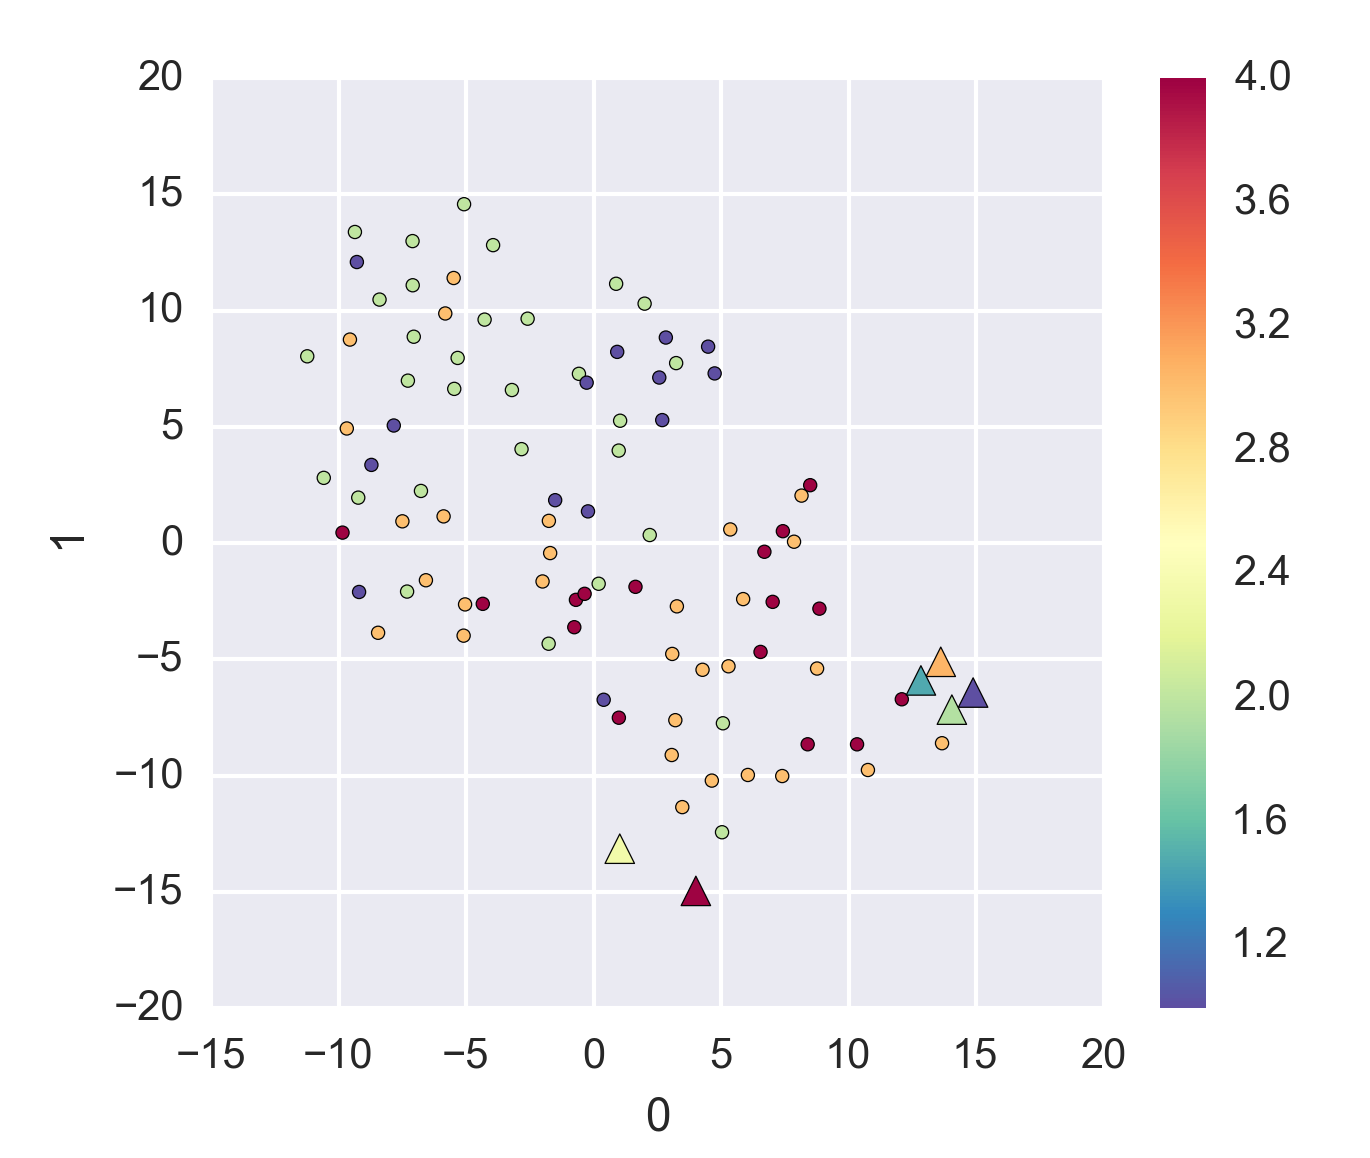
\includegraphics[width=0.49\textwidth]{figures/mappings/blob_SNE_mapping_2d.png}}
	\subfigure{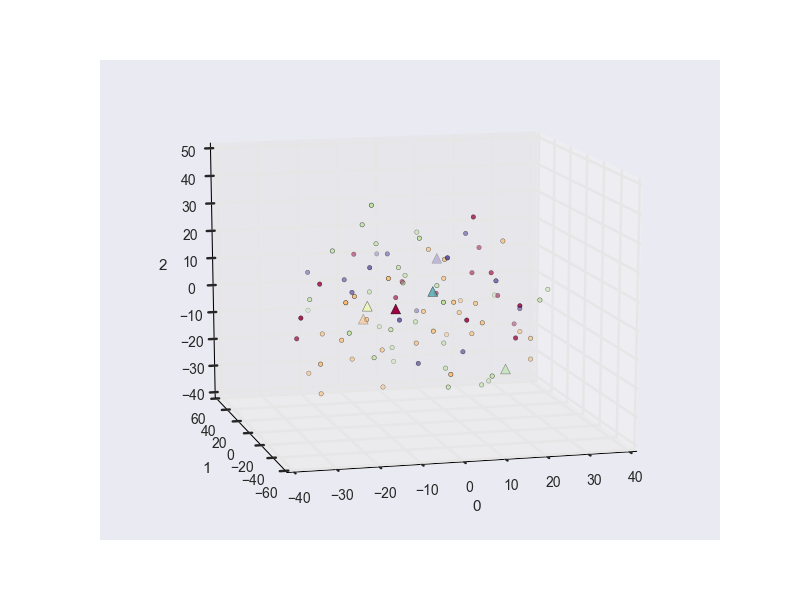
\includegraphics[width=0.49\textwidth]{figures/mappings/blob_SNE_mapping_3d.png}}
	\caption{2D \& 3D projections of the blob feature space produced by the t-SNE algorithm with a learning rate of 300 and perplexity of 30.}\label{fig:blob_SNE_mapping}
\end{figure}

\begin{figure}[H]
	\centering
	\subfigure{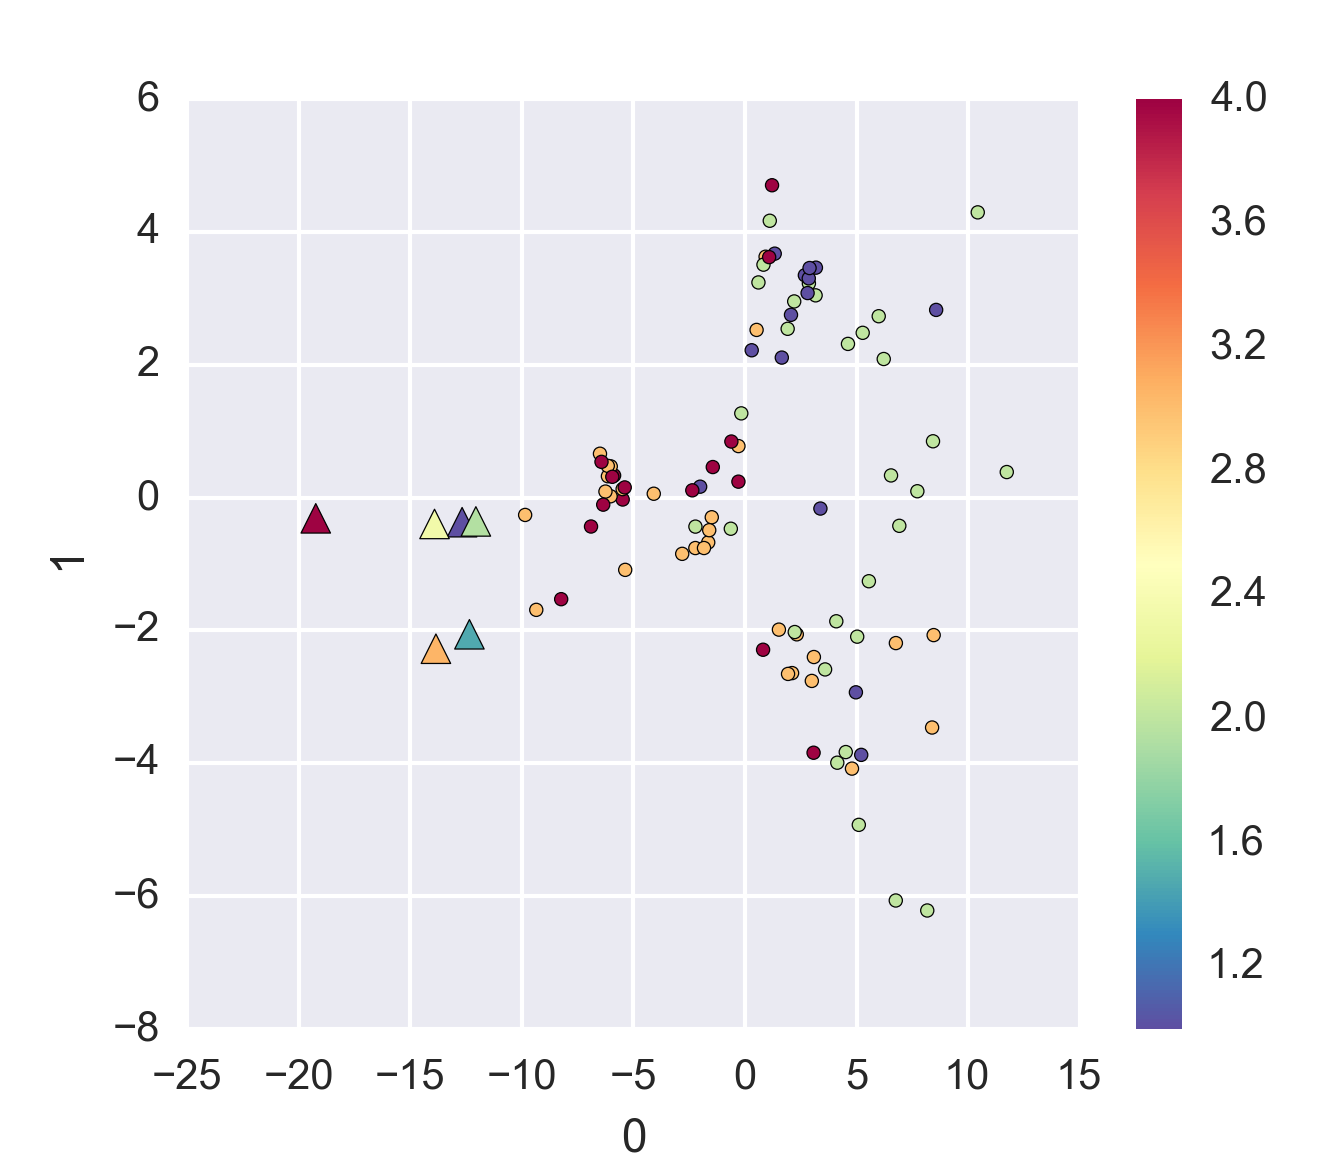
\includegraphics[width=0.49\textwidth]{figures/mappings/blob_iso_mapping_2d.png}}
	\subfigure{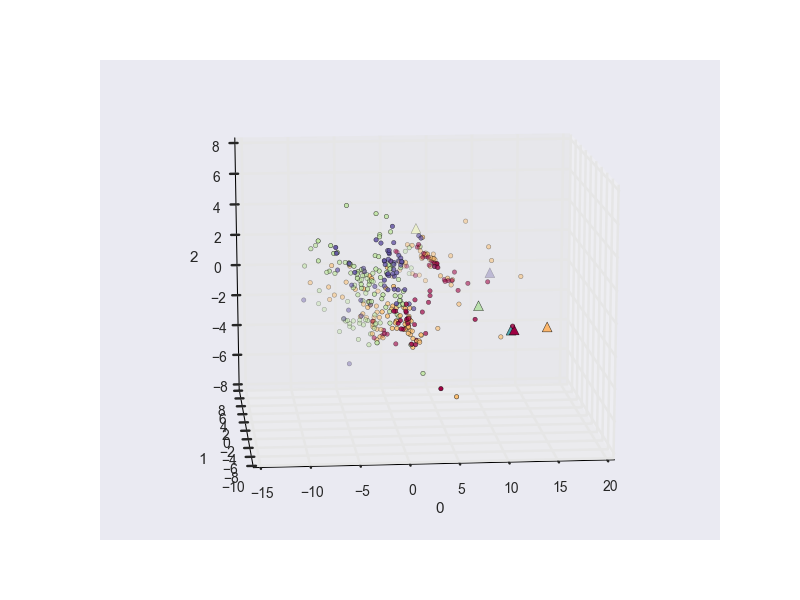
\includegraphics[width=0.49\textwidth]{figures/mappings/blob_iso_mapping_3d.png}}
	\caption{2D \& 3D projections of the blob feature space  produced by the Isomap algorithm with 10 neighbours.}\label{fig:blob_iso_mapping}
\end{figure}

\begin{figure}[H]
	\centering
	\subfigure{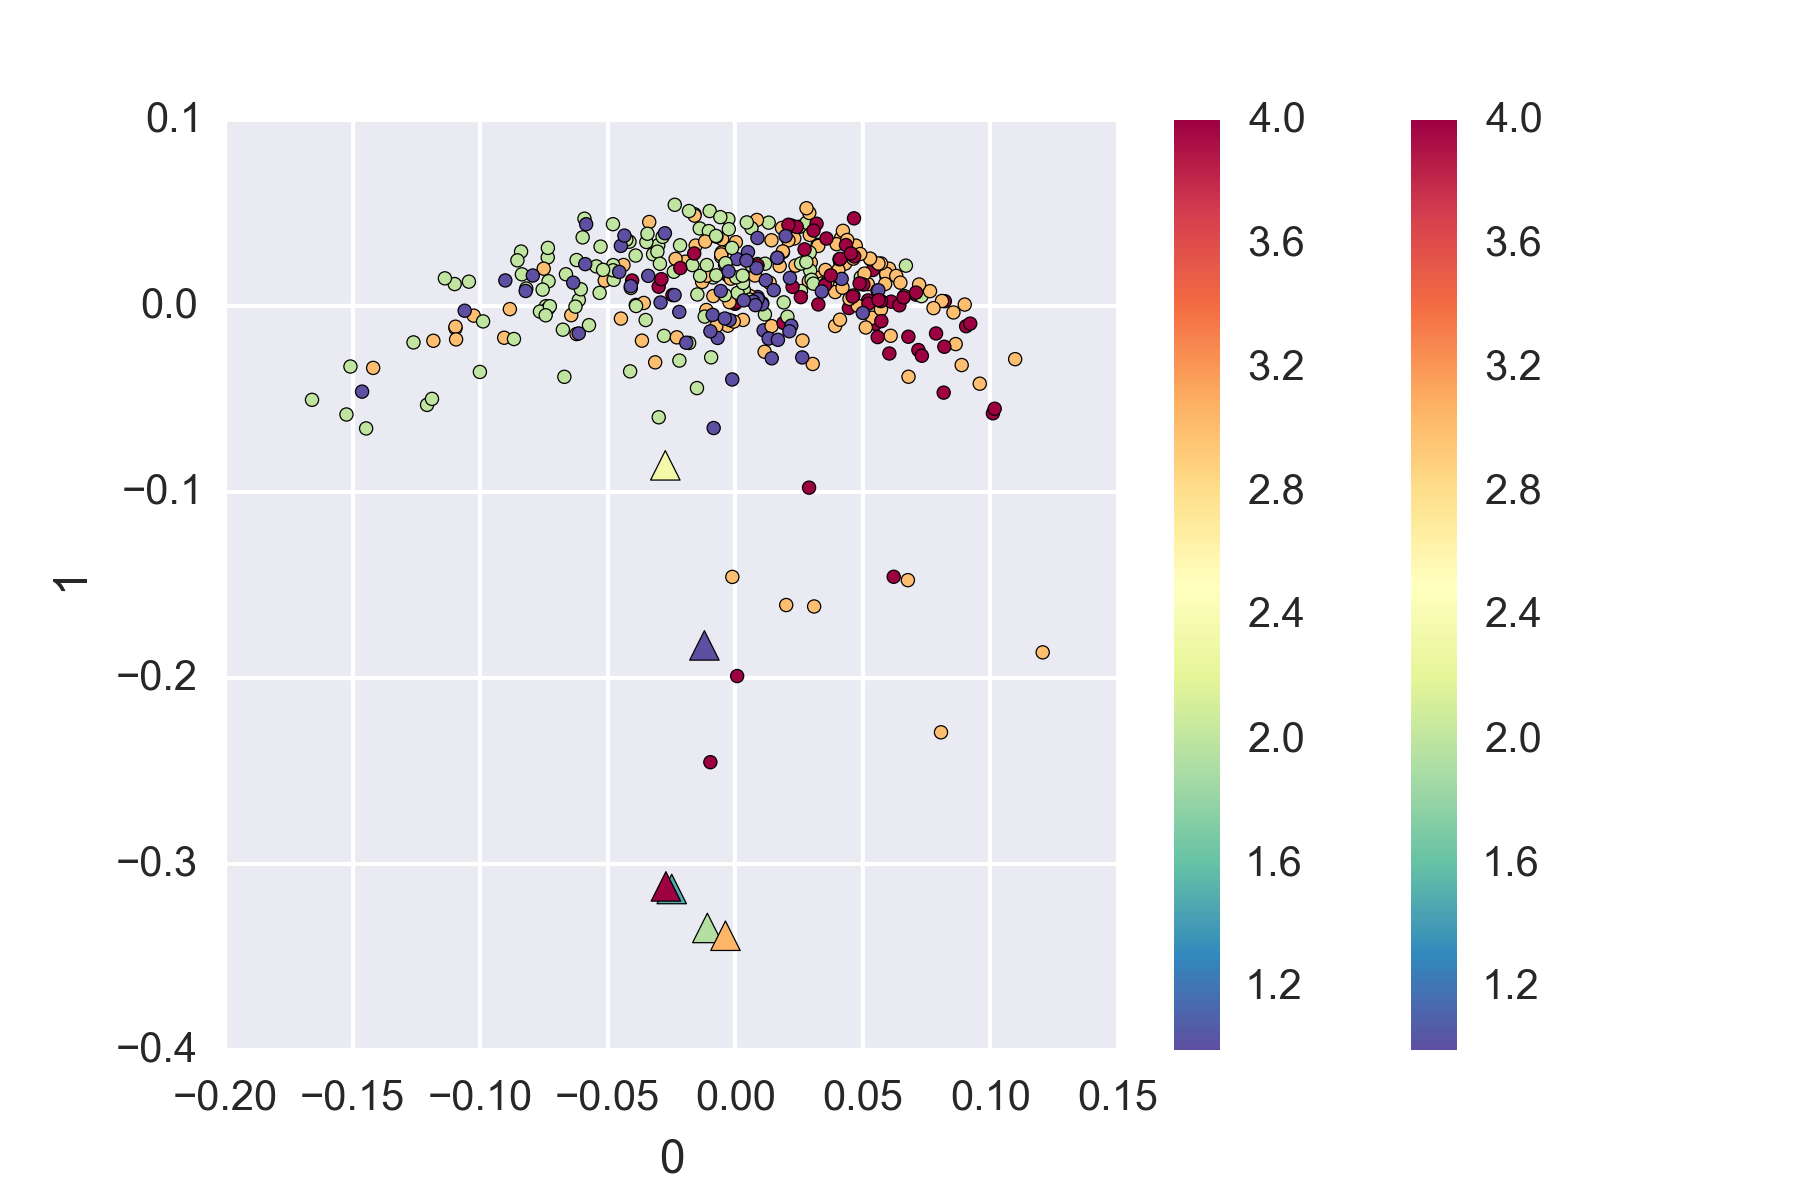
\includegraphics[width=0.49\textwidth]{figures/mappings/blob_lle_mapping_2d.png}}
	\subfigure{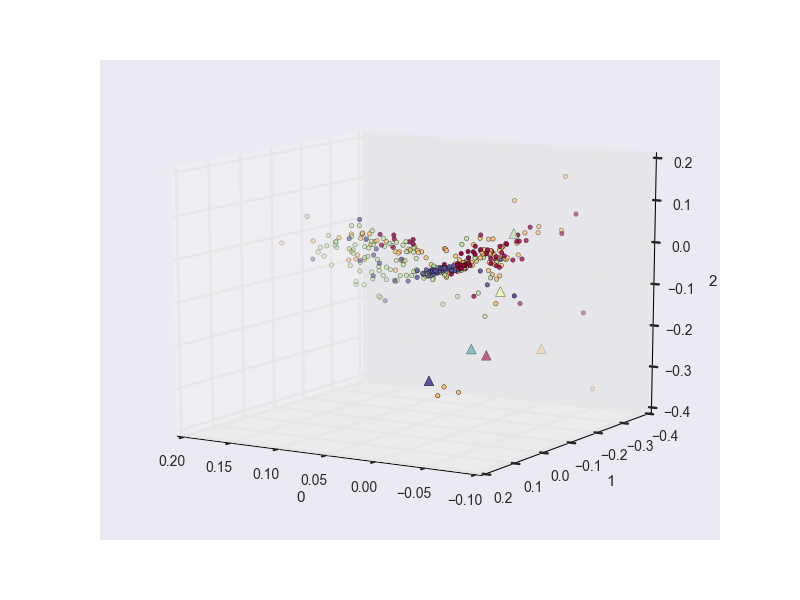
\includegraphics[width=0.49\textwidth]{figures/mappings/blob_lle_mapping_3d.png}}
	\caption{2D \& 3D projections of the blob feature space produced by the LLE algorithm with 10 neighbours.}\label{fig:blob_LLE_mapping}
\end{figure}
\clearpage

\clearpage
\begin{figure}[H]
	\centering
	\subfigure{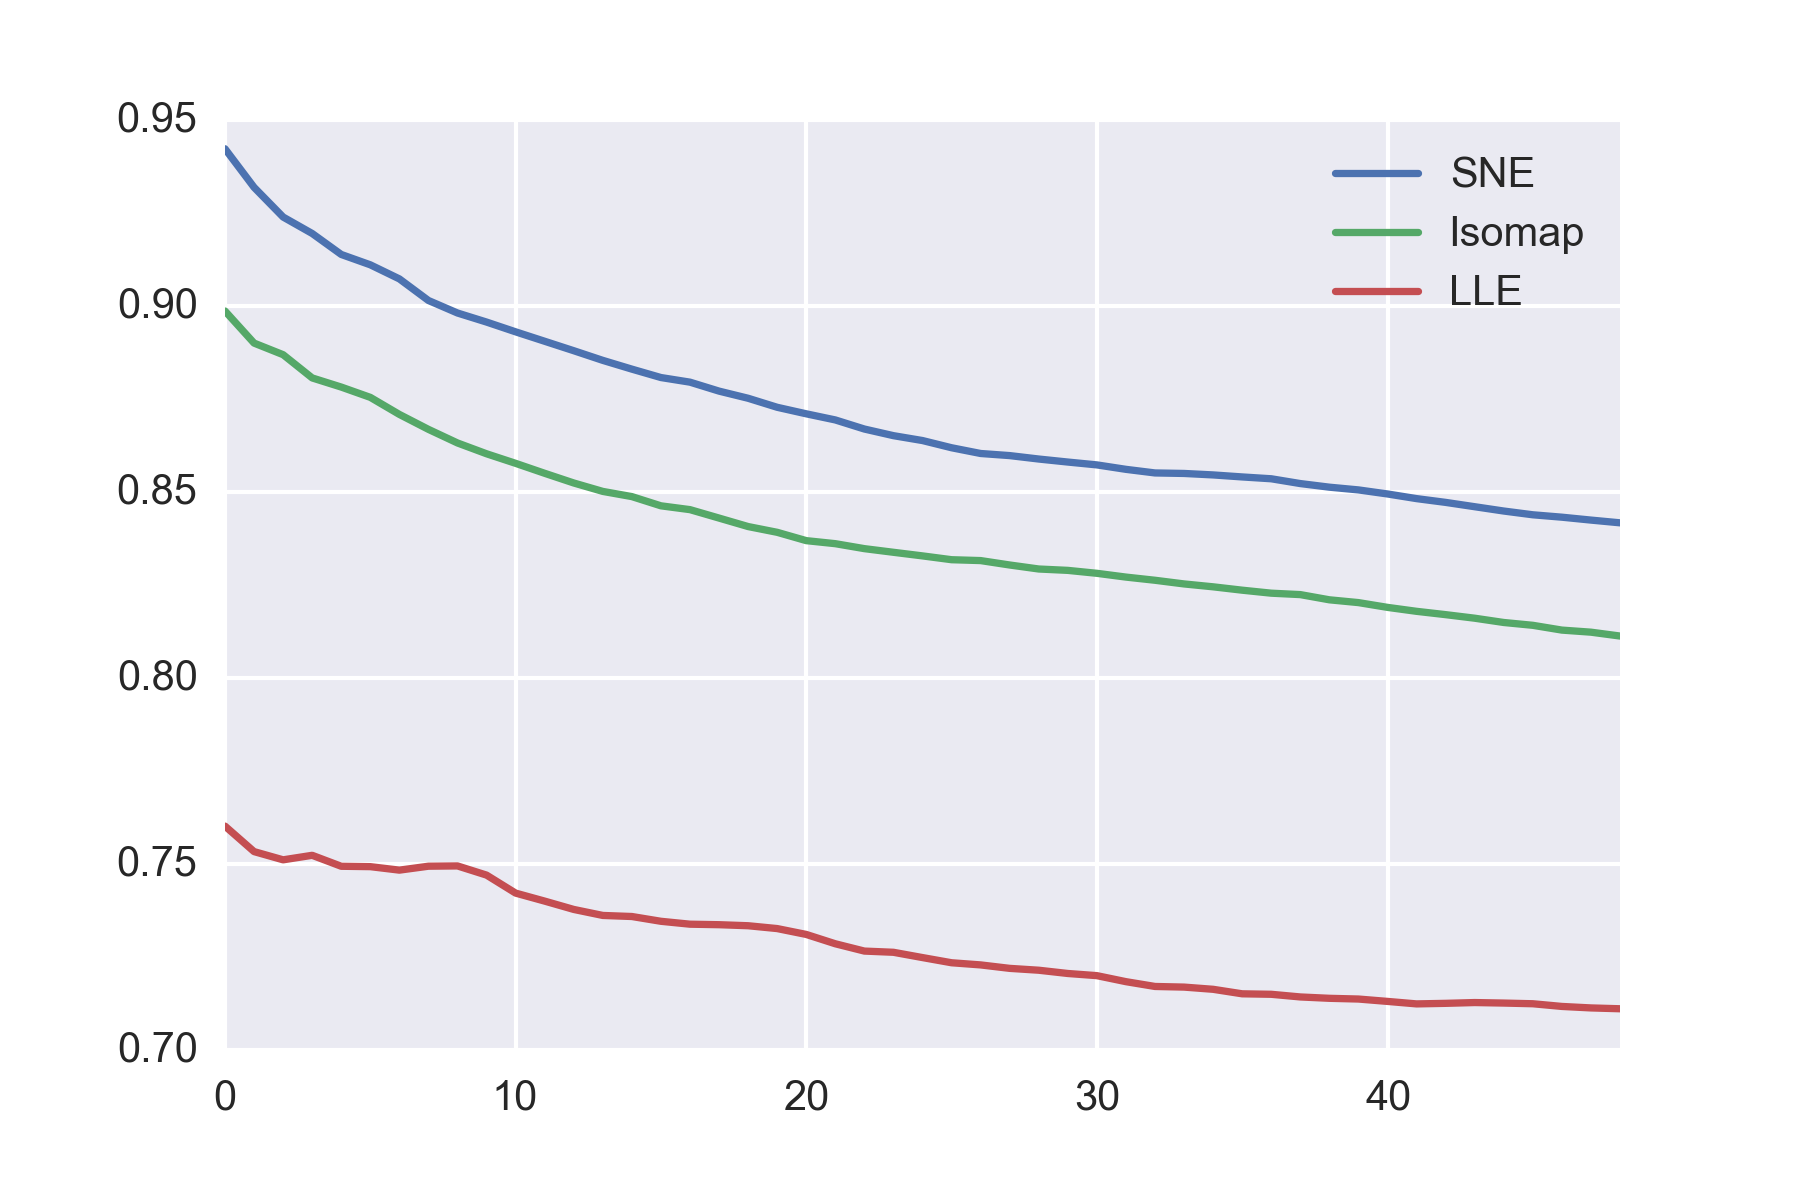
\includegraphics[width=0.49\textwidth]{figures/quality_measures/blob_trustworthiness_2d.png}}
	\subfigure{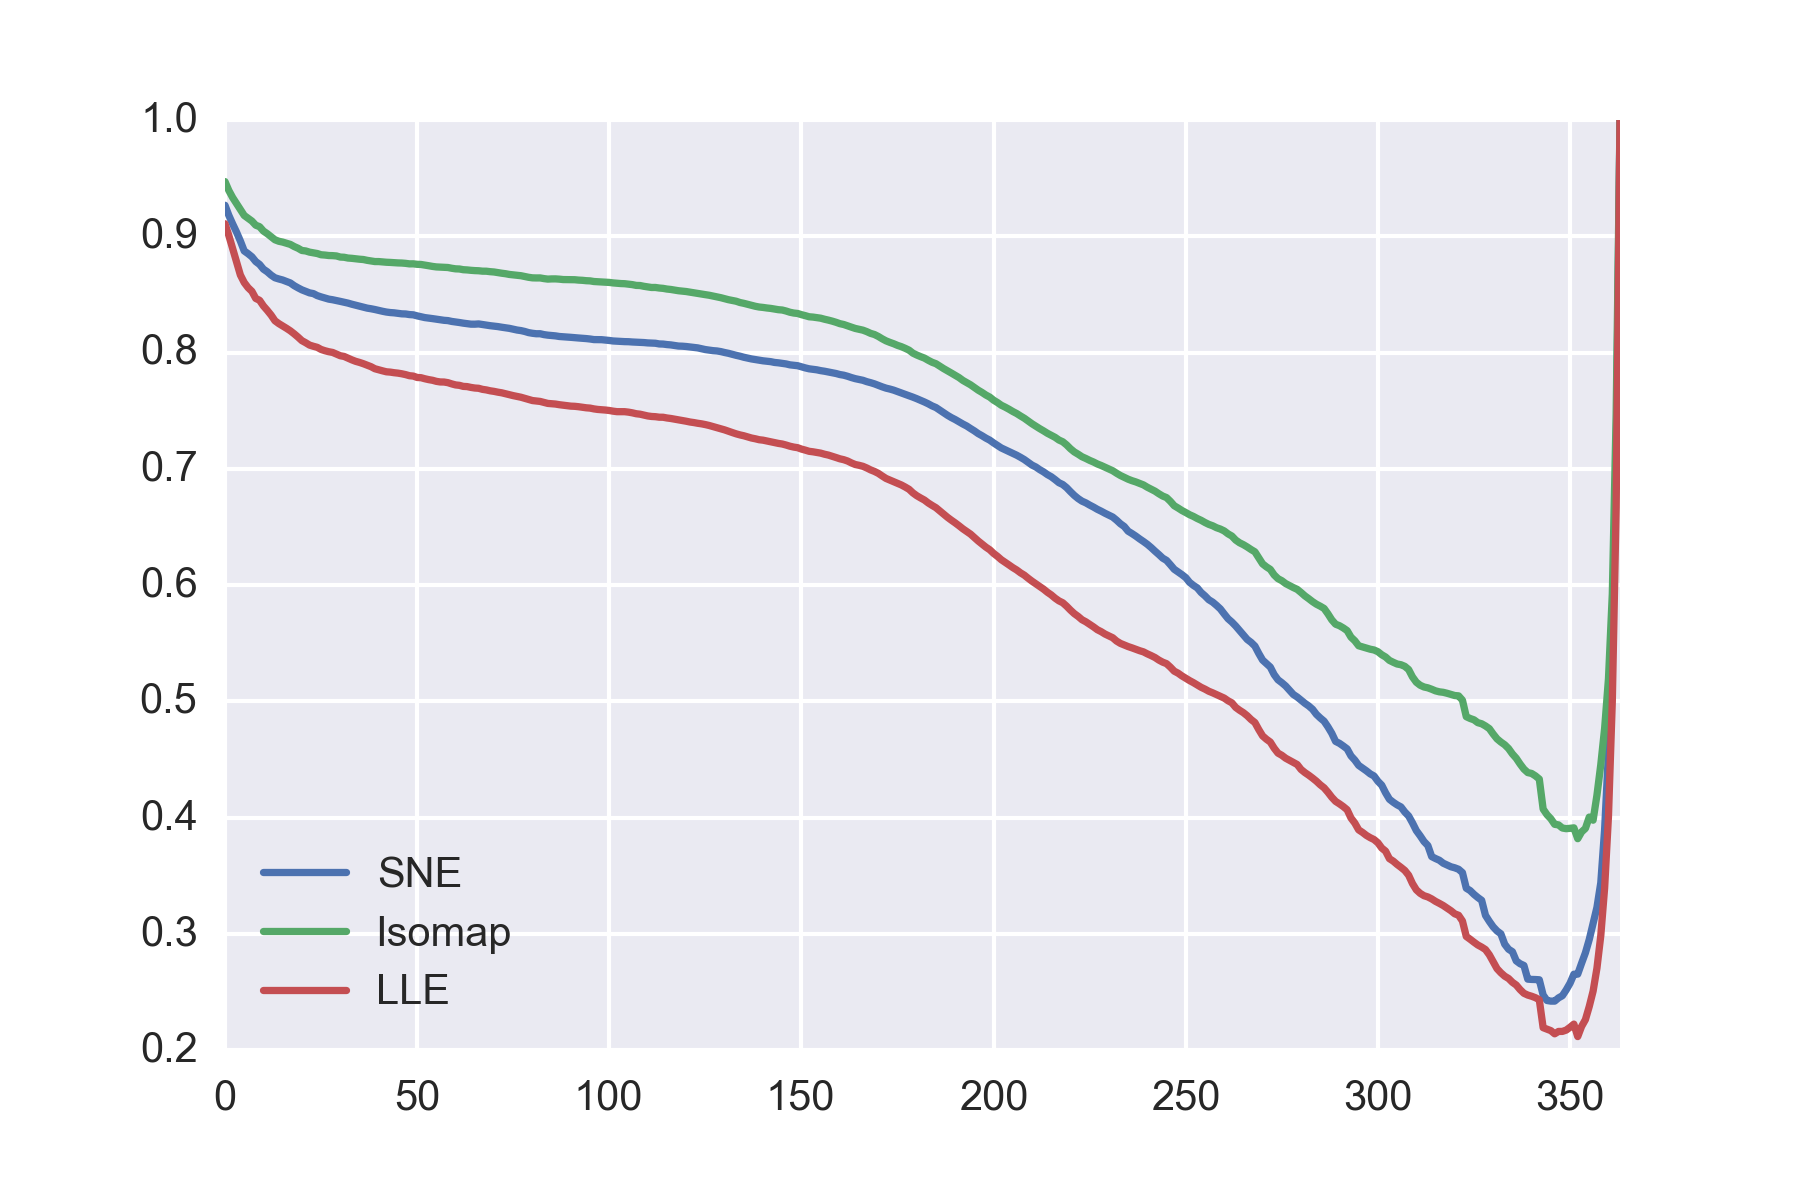
\includegraphics[width=0.49\textwidth]{figures/quality_measures/blob_continuity_2d.png}}
	\caption{Trustworthiness (left) and continuity (right) of the 2D projections produced from blob features.}\label{fig:TC_2d_blobs}
\end{figure}

\begin{figure}[H]
	\centering
	\subfigure{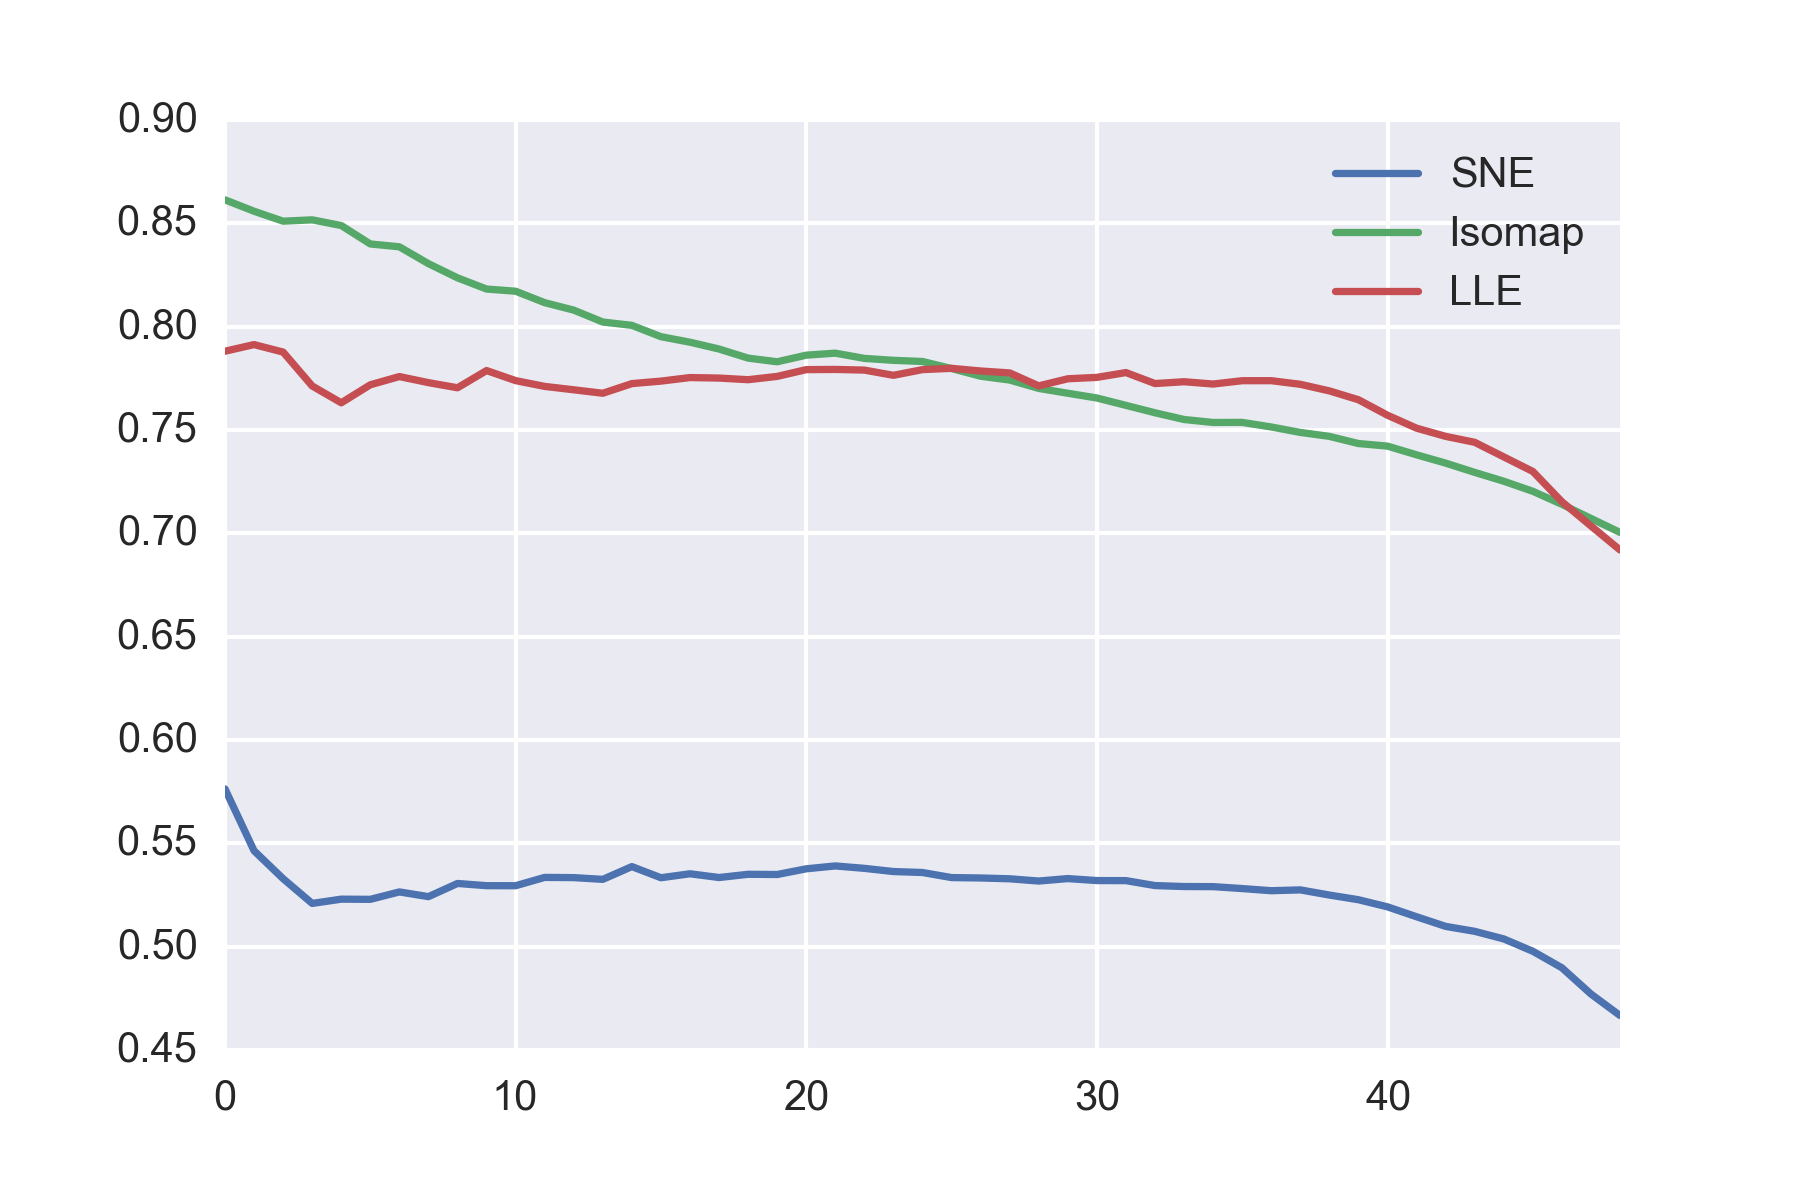
\includegraphics[width=0.49\textwidth]{figures/quality_measures/blob_trustworthiness_3d.png}}
	\subfigure{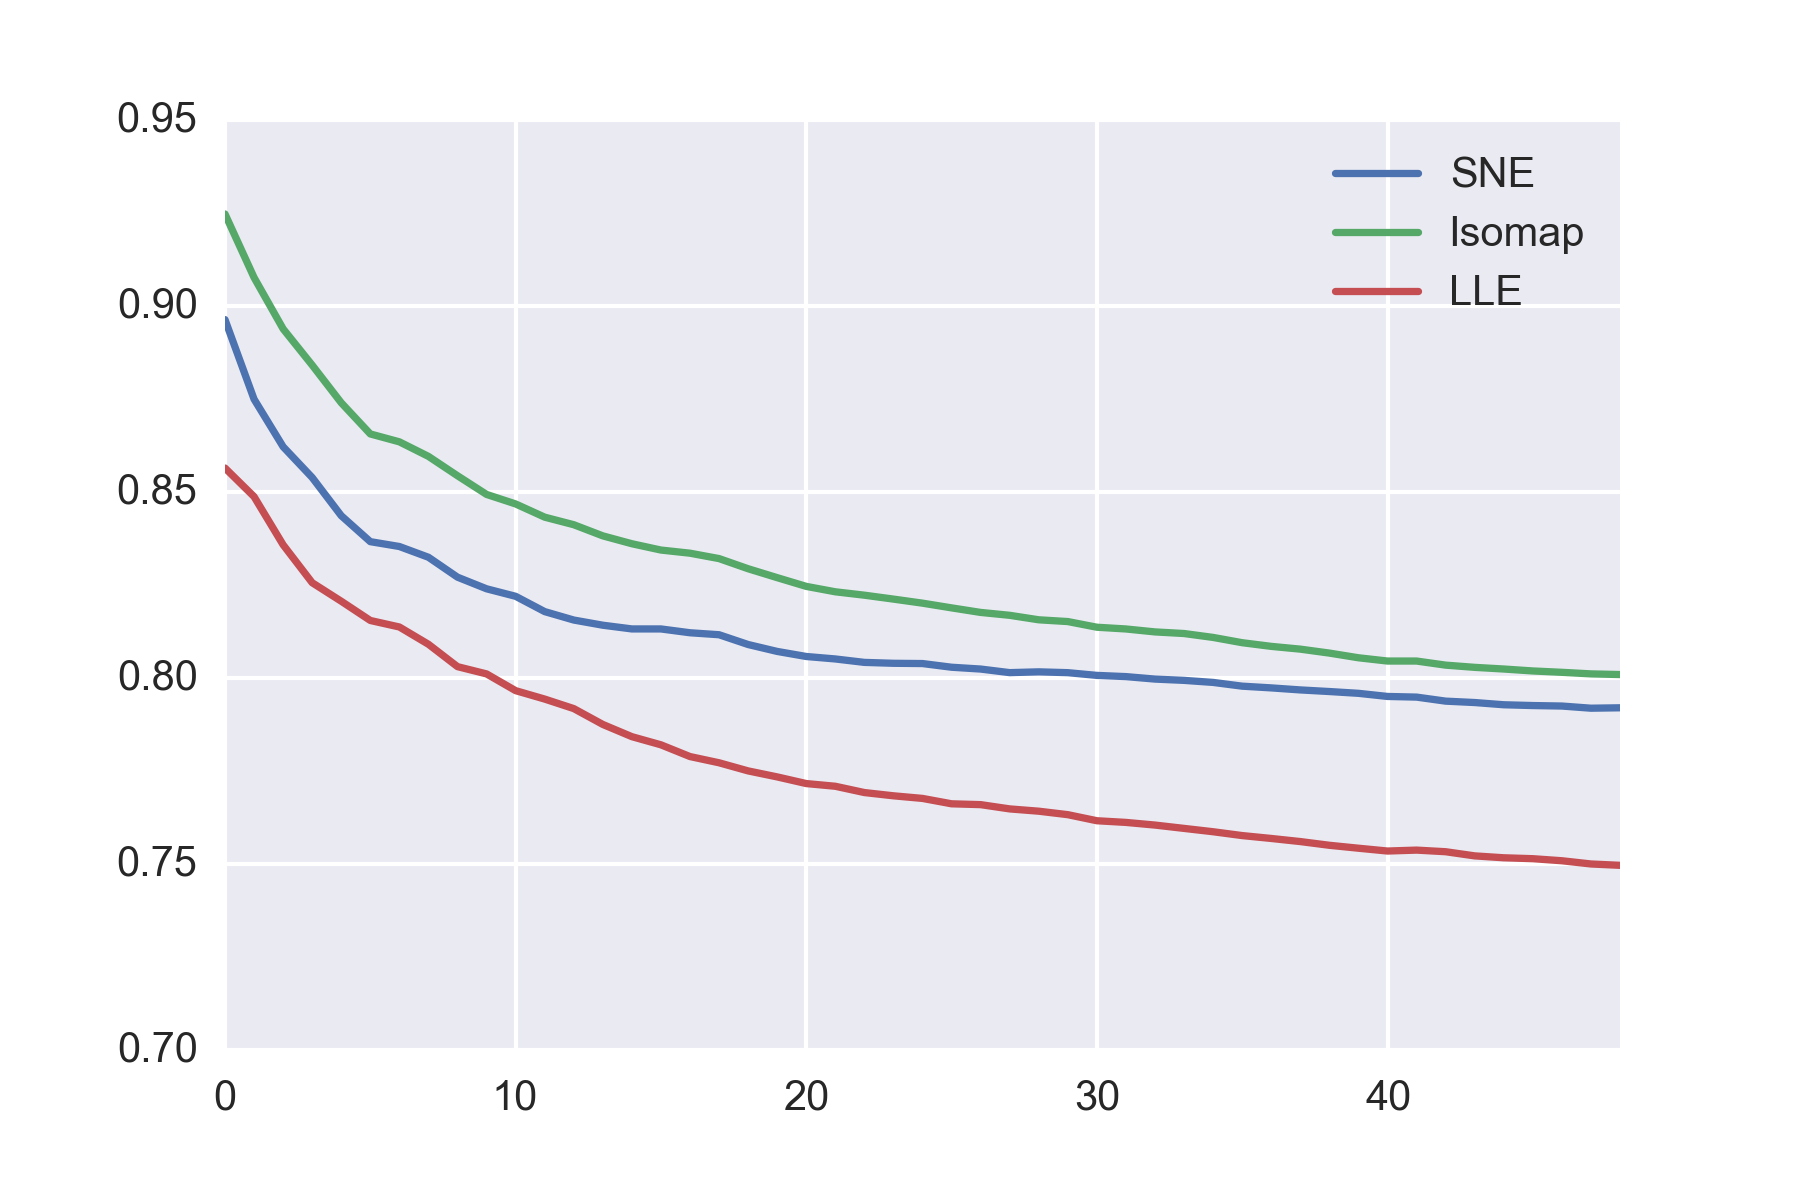
\includegraphics[width=0.49\textwidth]{figures/quality_measures/blob_continuity_3d.png}}
	\caption{Trustworthiness (left) and continuity (right) of the 3D projections produced from blob features.}\label{fig:TC_3d_blobs}
\end{figure}

\begin{figure}[H]
	\centering
	\subfigure{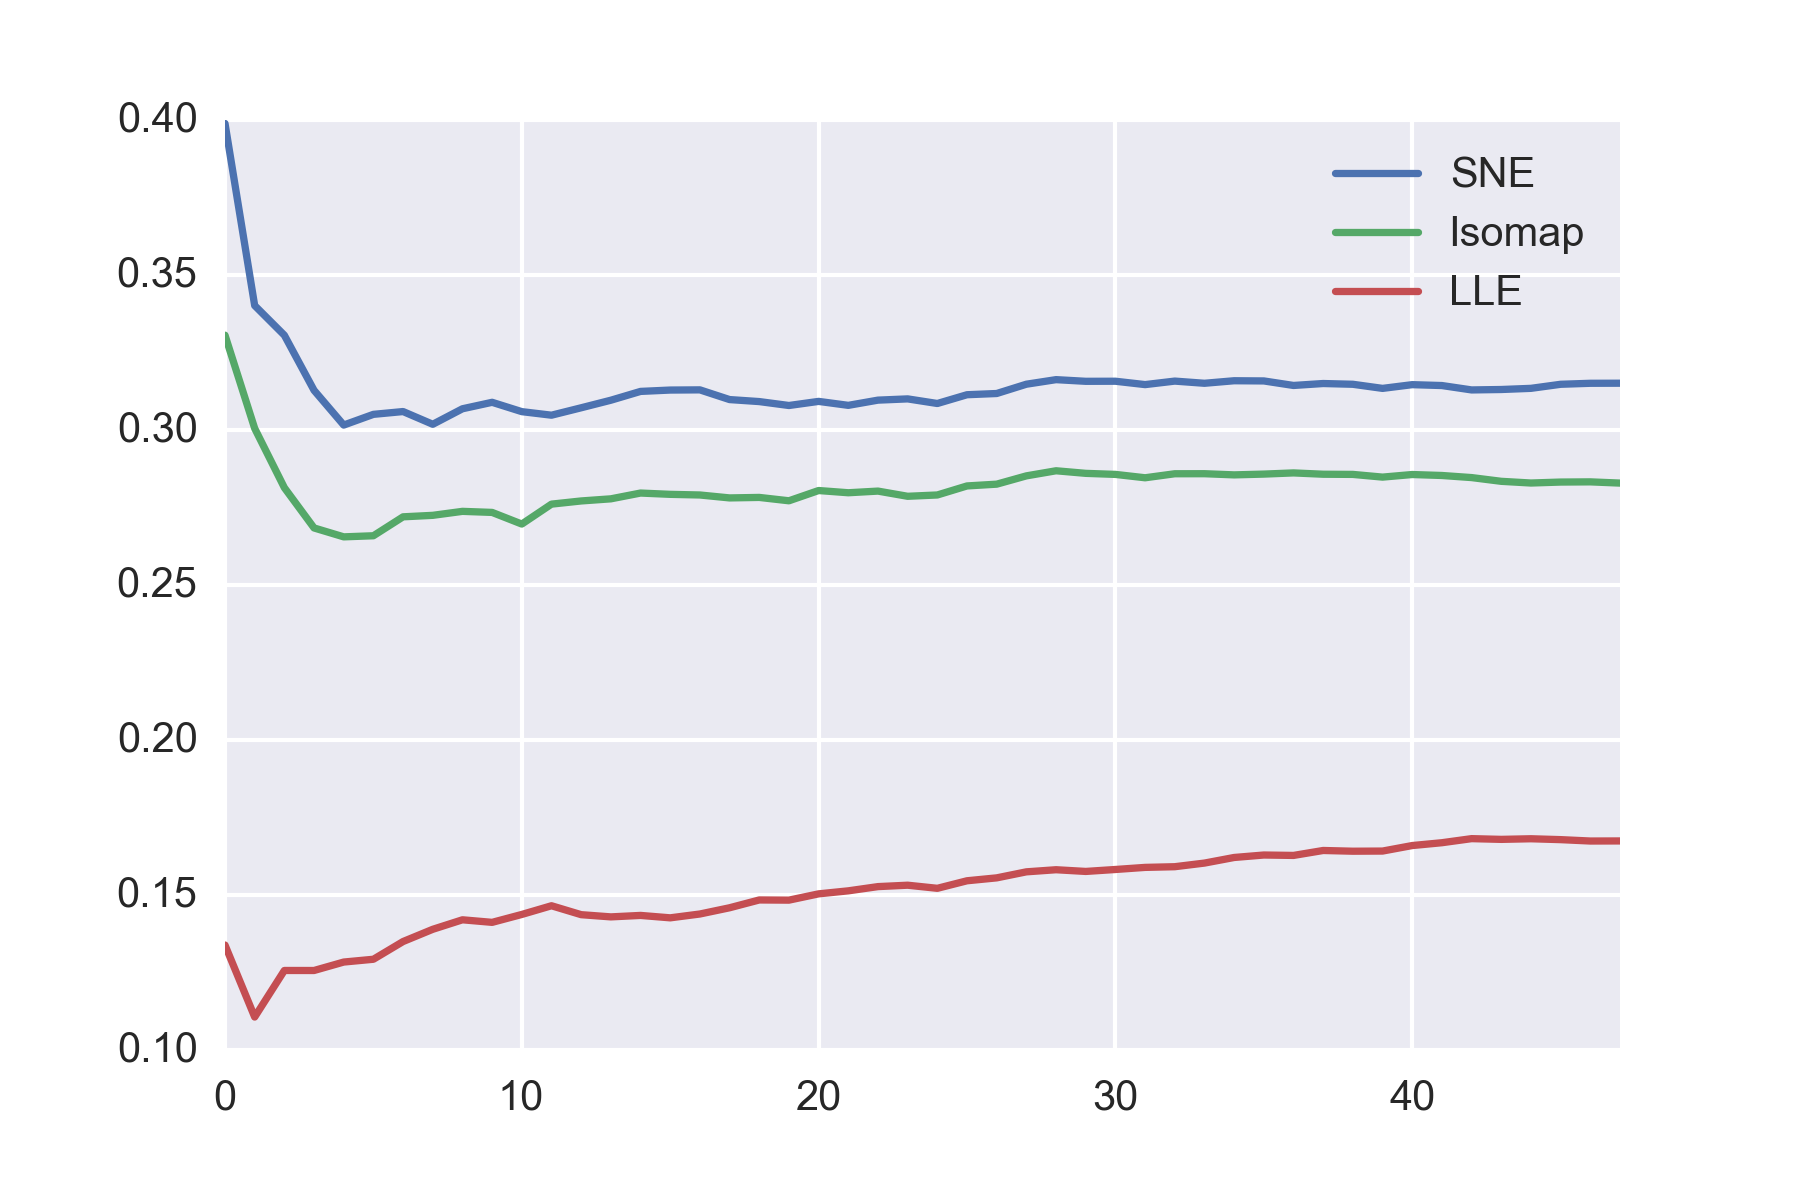
\includegraphics[width=0.49\textwidth]{figures/quality_measures/blob_lcmc_2d.png}}
	\subfigure{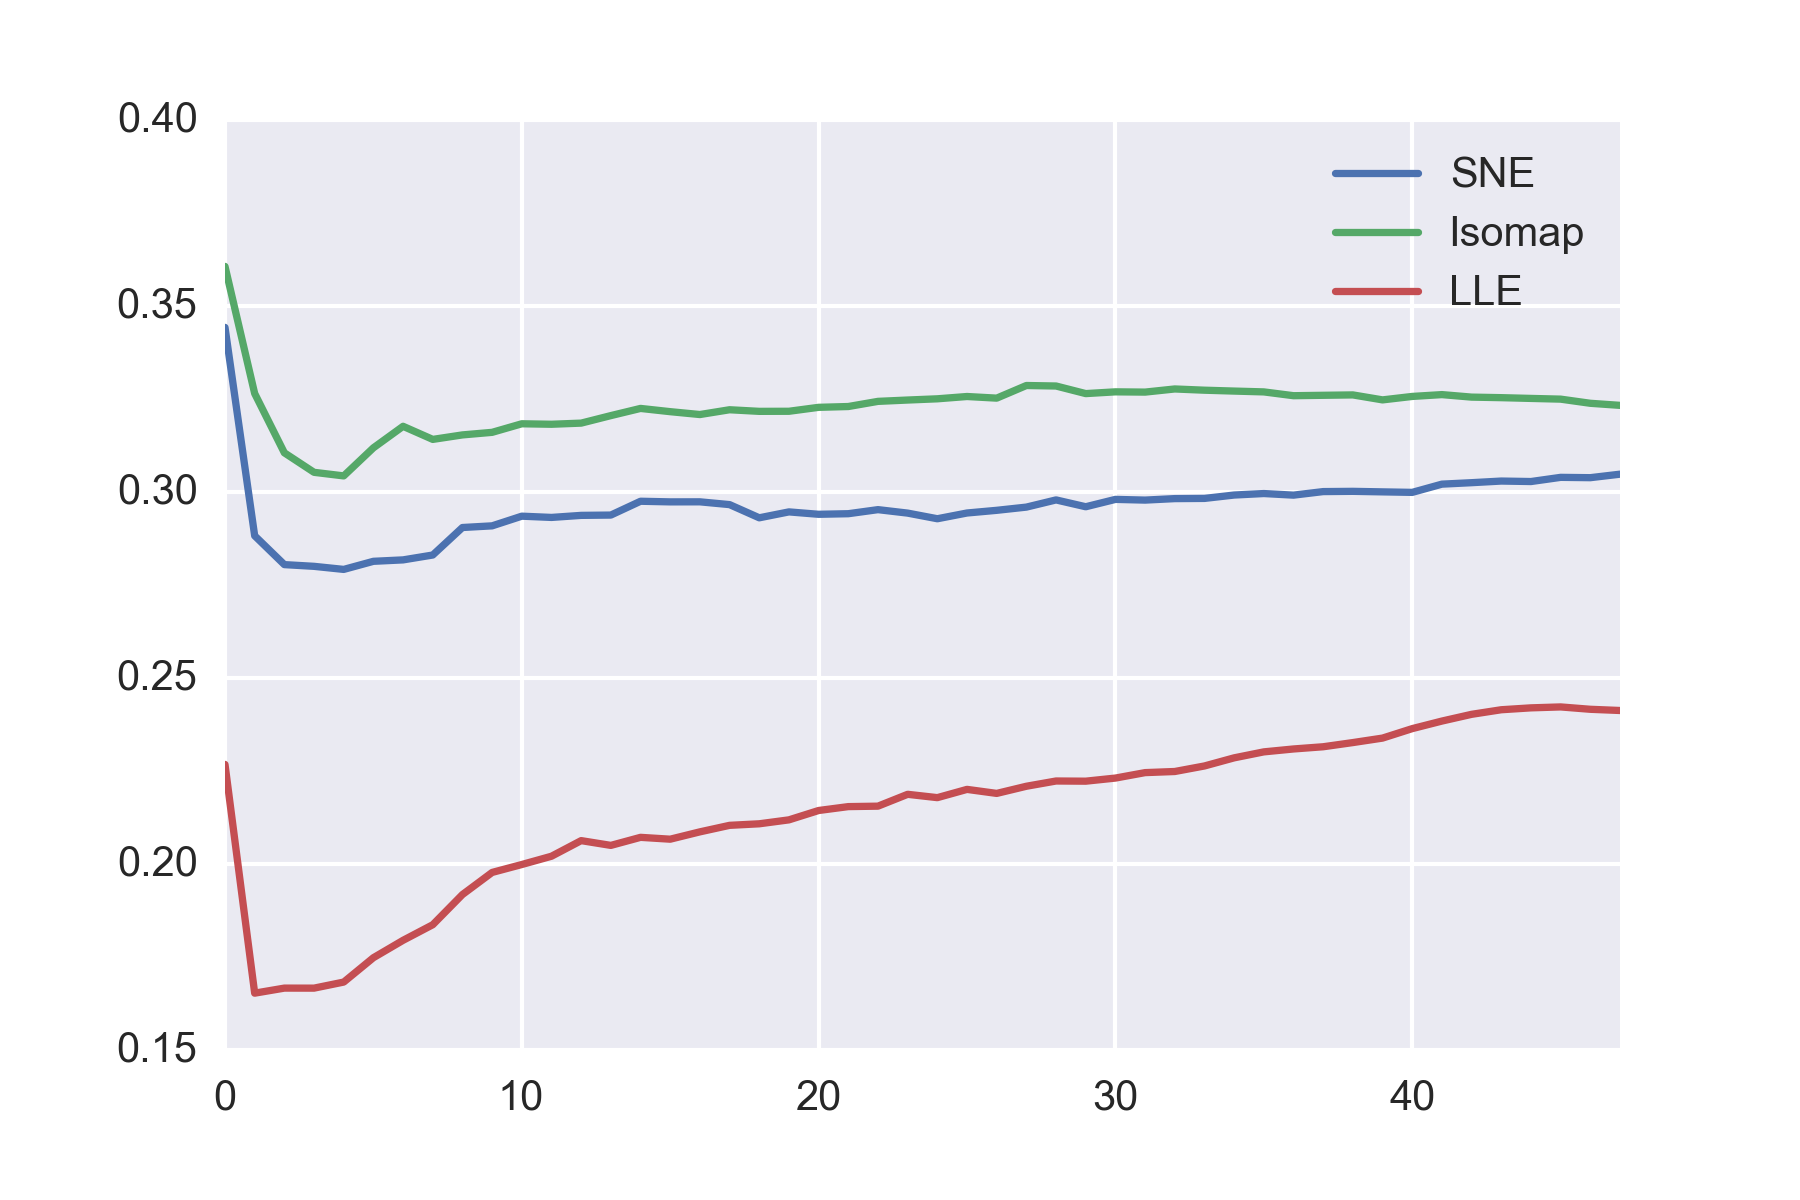
\includegraphics[width=0.49\textwidth]{figures/quality_measures/blob_lcmc_3d.png}}
	\caption{LCMC of both the 2D projection (left) and 3D projection (right) of the feature space for blobs.}\label{fig:LCMC_blobs}
\end{figure}
\clearpage

\subsection{Line features}
Results for the KS two sample test between the two feature spaces can be seen in table \ref{table:line_features_ks}. Again, as with blobs, the distributions for real and synthetic mammograms are not in particularly good agreement according to the test. 2D and 3D projections for the line feature space for each of the three different dimensionality reduction algorithms are shown in figures \ref{fig:line_SNE_mapping}, \ref{fig:line_iso_mapping}, and \ref{fig:line_LLE_mapping} respectively.
 
Note that in these results the value of the min area feature was removed. When using the min area feature all projections would produce two clusters. One smaller cluster would be created containing which contained blobs where the min area was much larger than the rest of the dataset. This is most likely caused by a thresholding issue causing some unwanted smaller lines to be retained for some of the images.

\begin{table}[H]
\label{table:line_features_ks}
\centering
\primitiveinput{tables/line_features_ks}
\caption{Comparison of the Kolmogorov-Smirnov test results for each feature generated from the area of lines detected in an image between real and phantom mammograms.}
\end{table}

The t-SNE projection shows that there is a general transition from images which contain a high mean area of linear structure on the left towards images which have a lower mean area on the right. In terms of BIRADS risk it can be seen that very low and very high risk classes are grouped towards the left, reflecting that less liner structure is detected using the orientated bins method in low risk classes (because there's very little dense structure present) and high risk classes (because dense areas are mostly large, homogenous blobs not linear structure). As can be clearly seen from the visualisation the synthetic images are grouped towards the lower end reflecting the smaller size of the linear structures detected. 

The projections produced by LLE and Isomap produce contain far less visible structure in comparison to t-SNE. Both techniques produce a fairly structureless blob with some transition between the low \& high risk to middle risk cases. This less obvious transition is again explained by the same relationship that is present in the t-SNE projection, but is just less prominent. The reduction in the quality of the projection could be down to the choice of $k$ or the crowding problem.

Examination of the three quality criteria show that t-SNE does not perform so well here when compared to the blob feature space. In general, Isomap provides a ``better" embedding according to the co-ranking metrics than the one produced by t-SNE for both 2D and 3D projections. In terms of trustworthiness and continuity t-SNE produces embeddings that are better in 2 dimensions in terms of the immediate neighbourhood but quickly degrades when measured against larger neighbourhoods.

\begin{figure}[H]
	\centering
	\subfigure{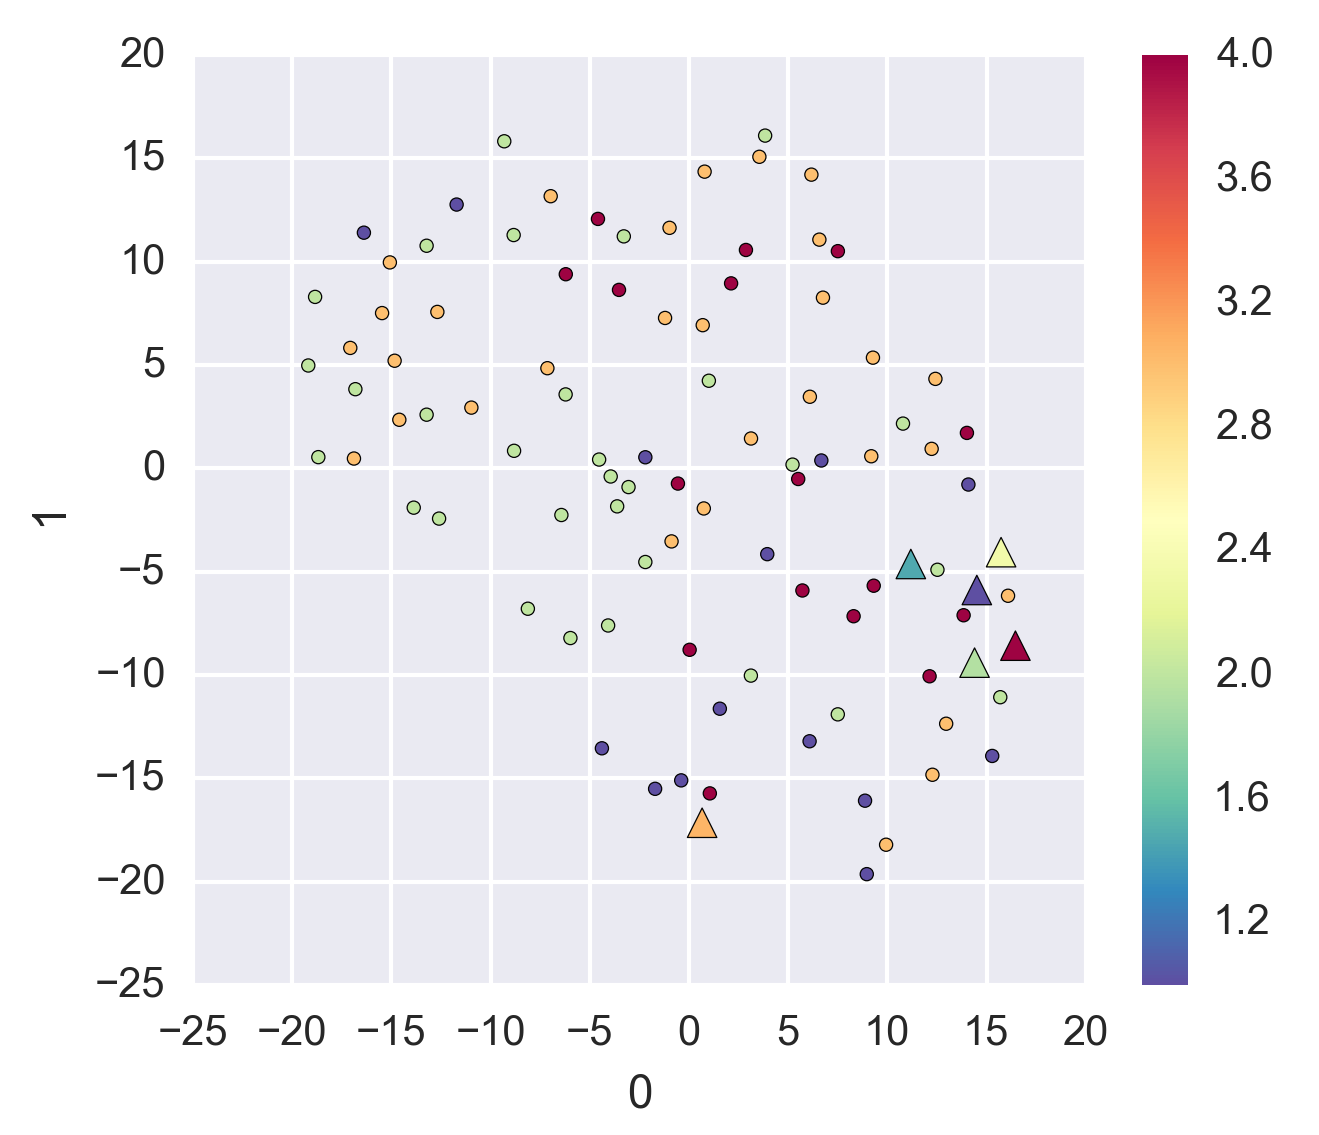
\includegraphics[width=0.49\textwidth]{figures/mappings/line_SNE_mapping_2d.png}}
	\subfigure{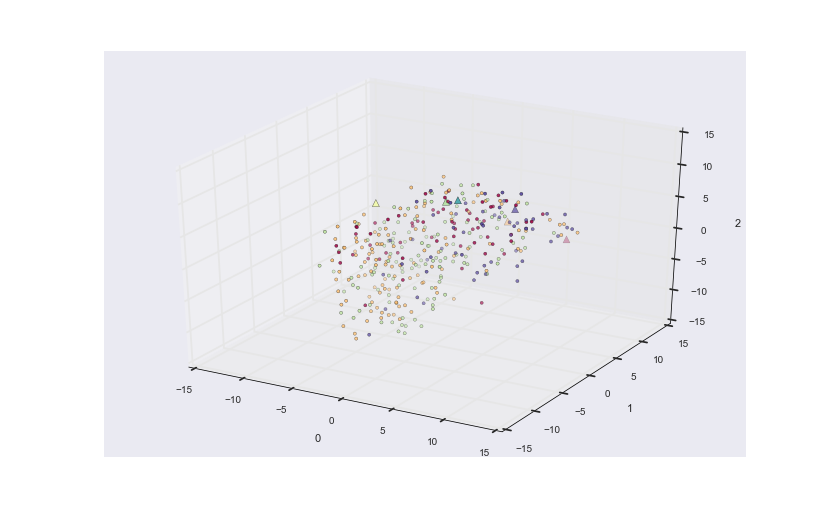
\includegraphics[width=0.49\textwidth]{figures/mappings/line_SNE_mapping_3d.png}}
	\caption{2D \& 3D projections of the line feature space produced by the t-SNE algorithm with a learning rate of 300 and perplexity of 30.}\label{fig:line_SNE_mapping}
\end{figure}

\begin{figure}[H]
	\centering
	\subfigure{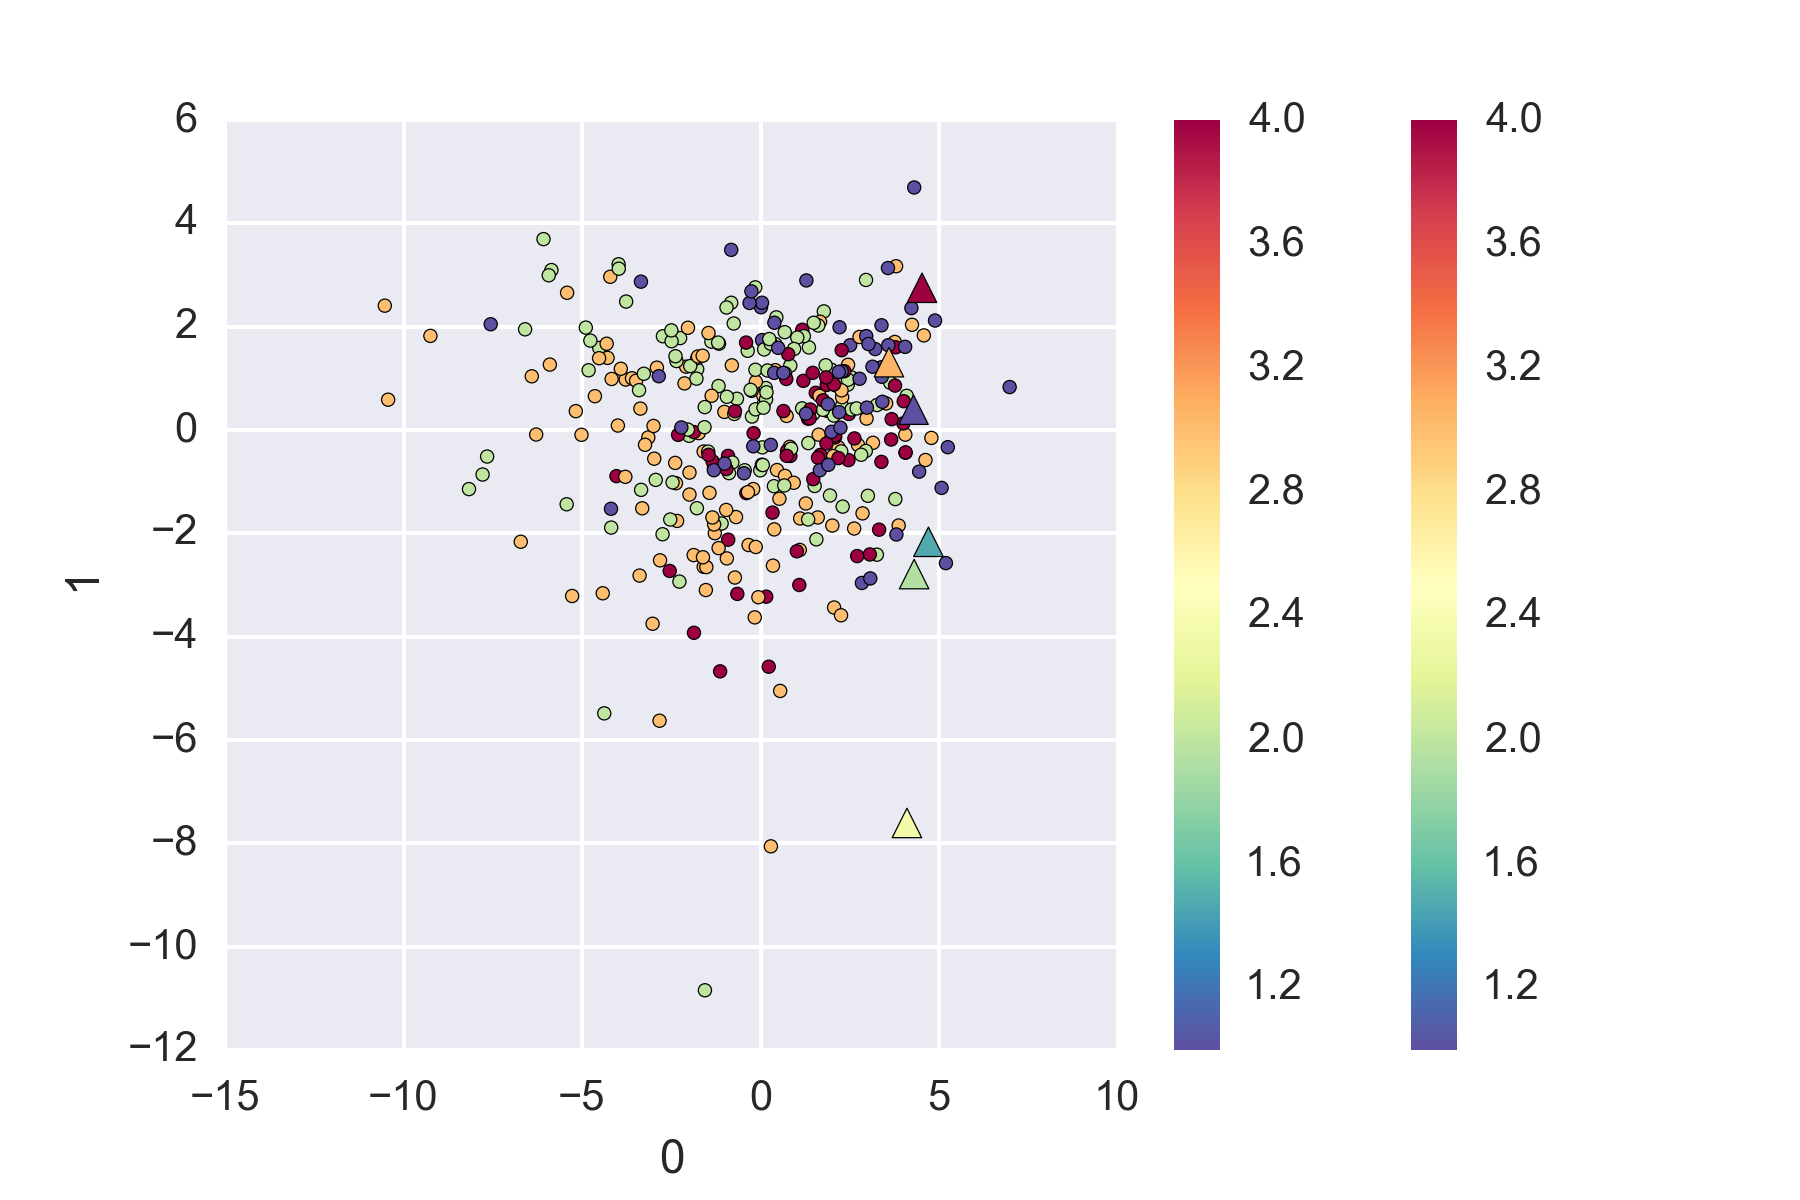
\includegraphics[width=0.49\textwidth]{figures/mappings/line_iso_mapping_2d.png}}
	\subfigure{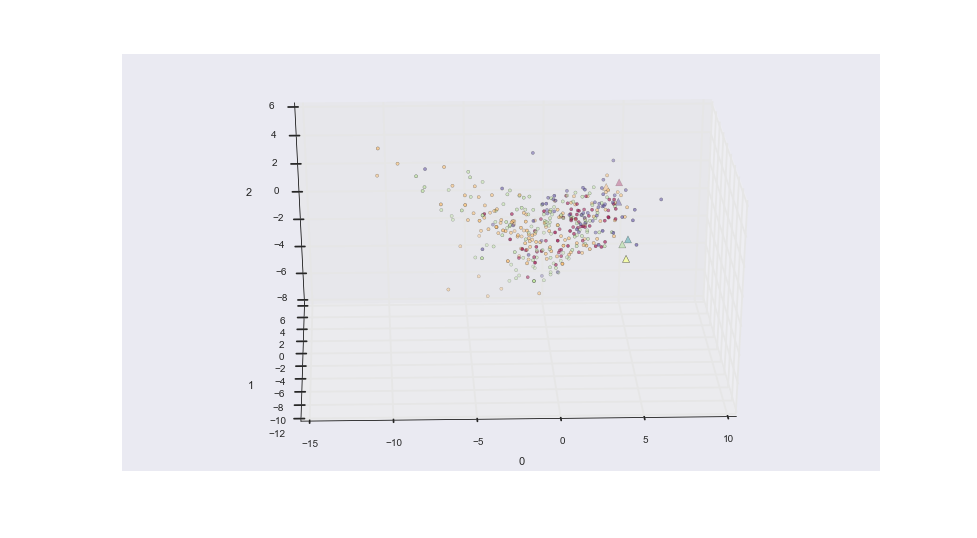
\includegraphics[width=0.49\textwidth]{figures/mappings/line_iso_mapping_3d.png}}
	\caption{2D \& 3D projections of the line feature space  produced by the Isomap algorithm with 10 neighbours.}\label{fig:line_iso_mapping}
\end{figure}

\begin{figure}[H]
	\centering
	\subfigure{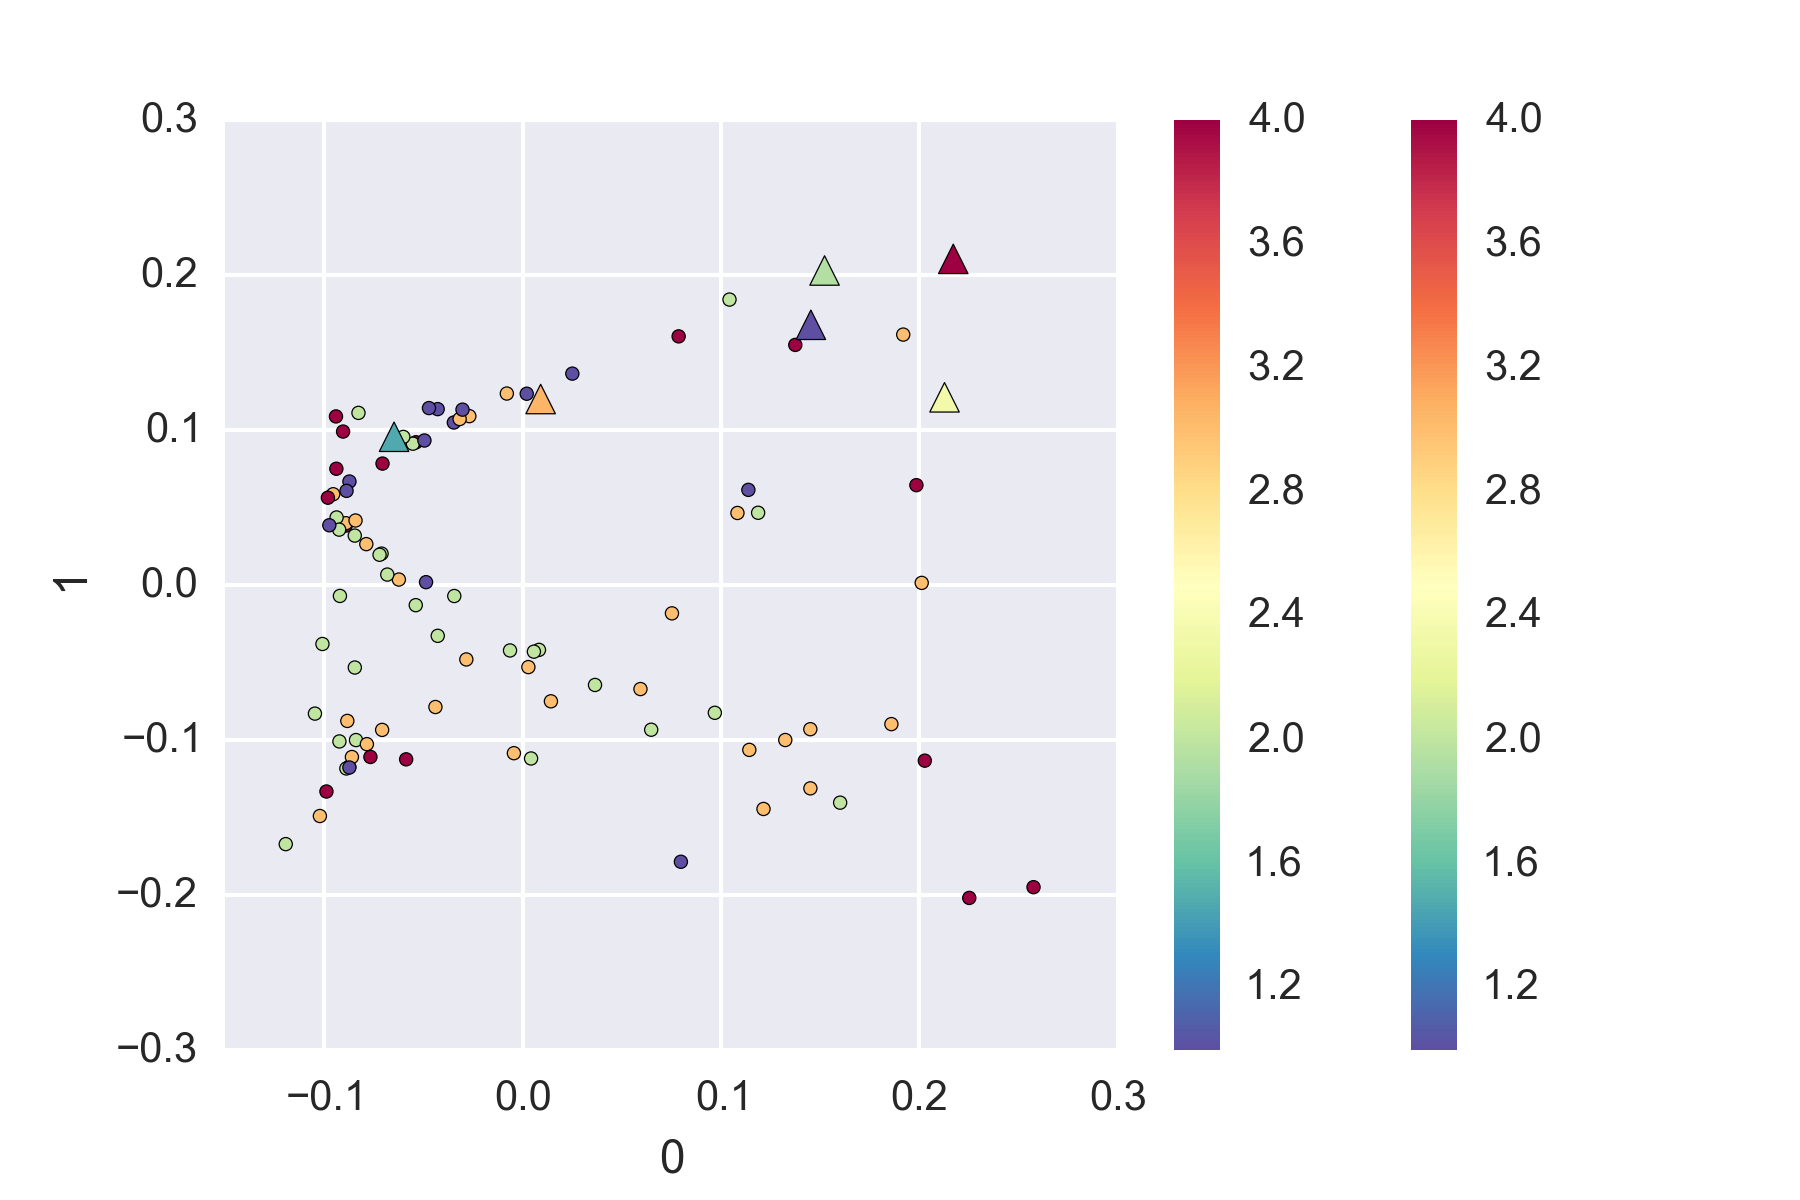
\includegraphics[width=0.49\textwidth]{figures/mappings/line_lle_mapping_2d.png}}
	\subfigure{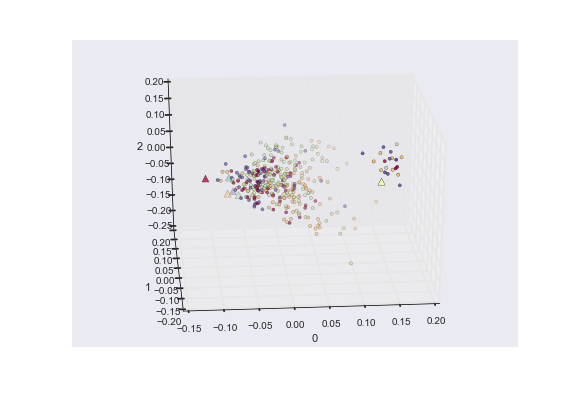
\includegraphics[width=0.49\textwidth]{figures/mappings/line_lle_mapping_3d.png}}
	\caption{2D \& 3D projections of the line feature space produced by the LLE algorithm with 10 neighbours.}\label{fig:line_LLE_mapping}
\end{figure}
\clearpage

\clearpage
\begin{figure}[H]
	\centering
	\subfigure{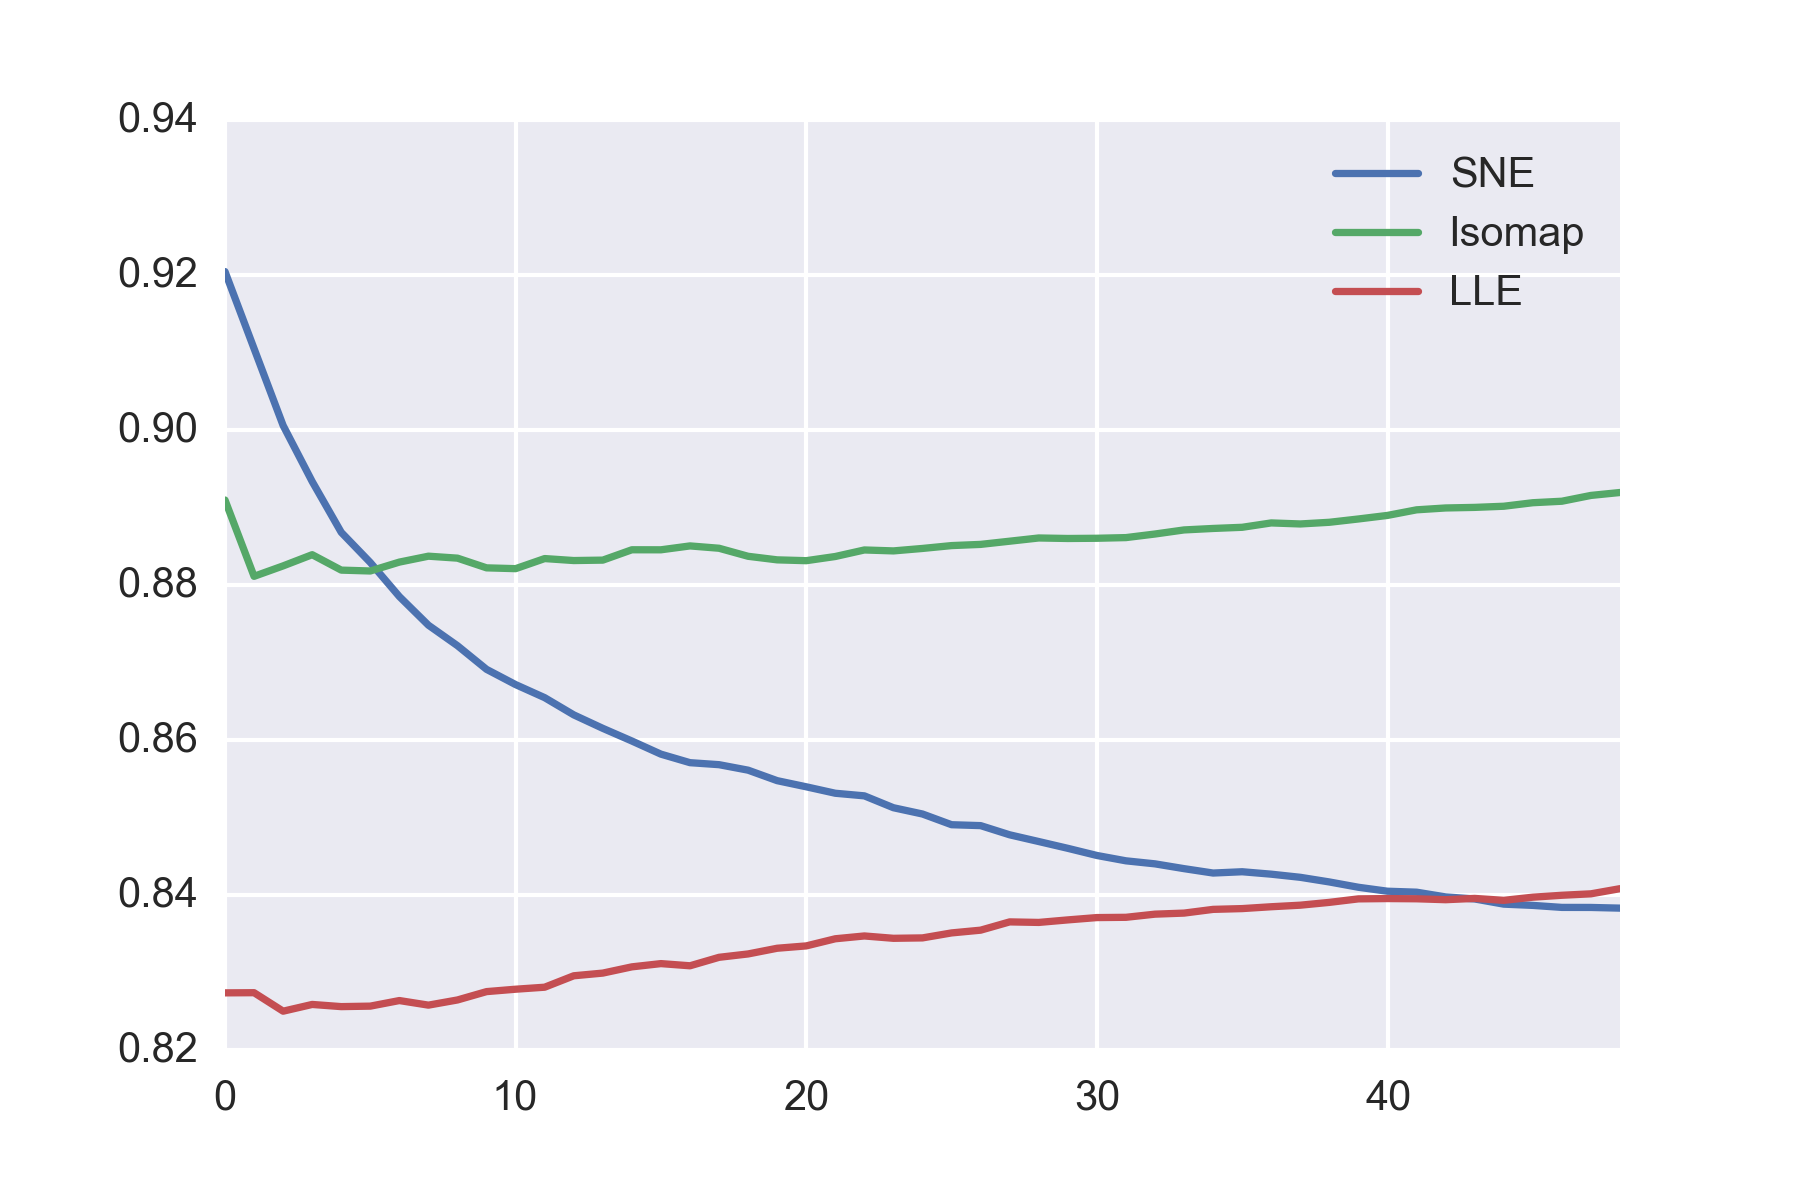
\includegraphics[width=0.49\textwidth]{figures/quality_measures/line_trustworthiness_2d.png}}
	\subfigure{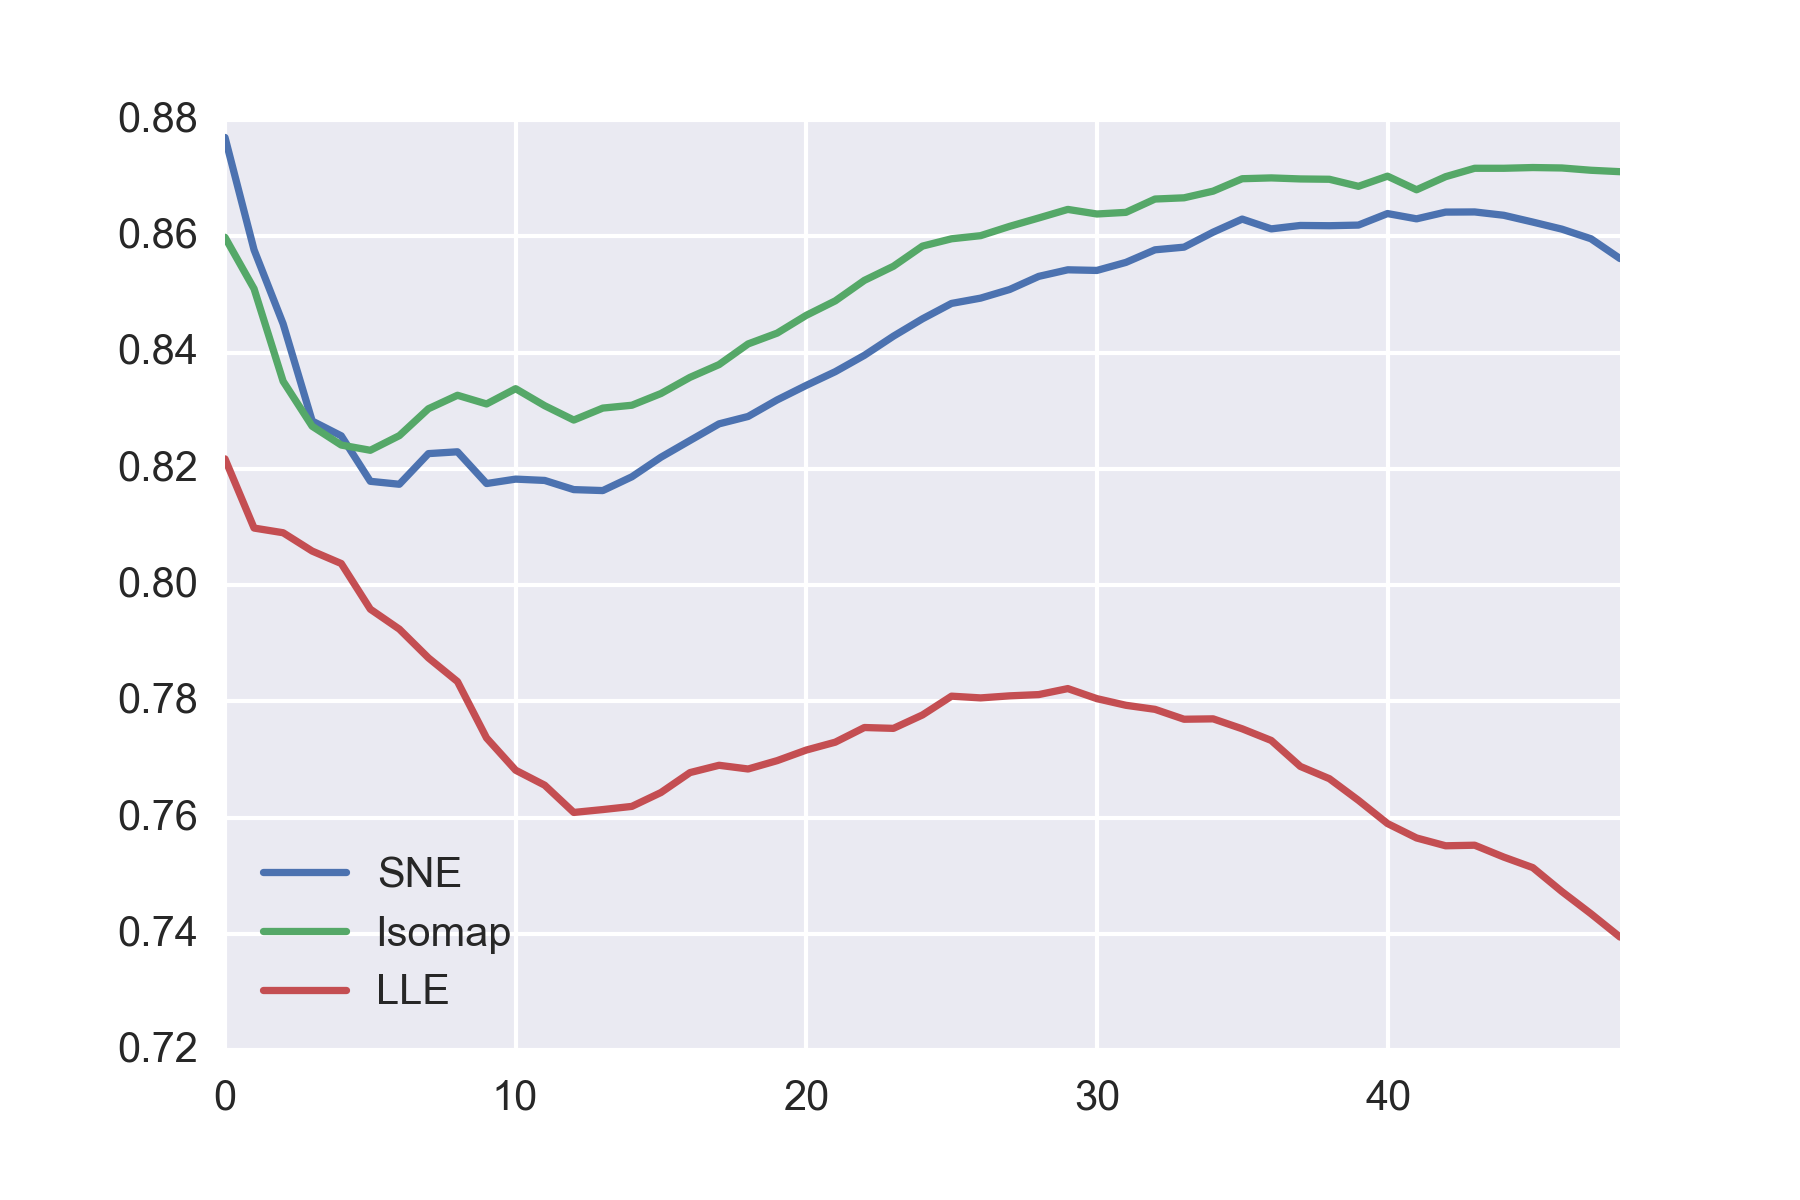
\includegraphics[width=0.49\textwidth]{figures/quality_measures/line_continuity_2d.png}}
	\caption{Trustworthiness (left) and continuity (right) of the 2D projections produced from line features.}\label{fig:TC_2d_lines}
\end{figure}

\begin{figure}[H]
	\centering
	\subfigure{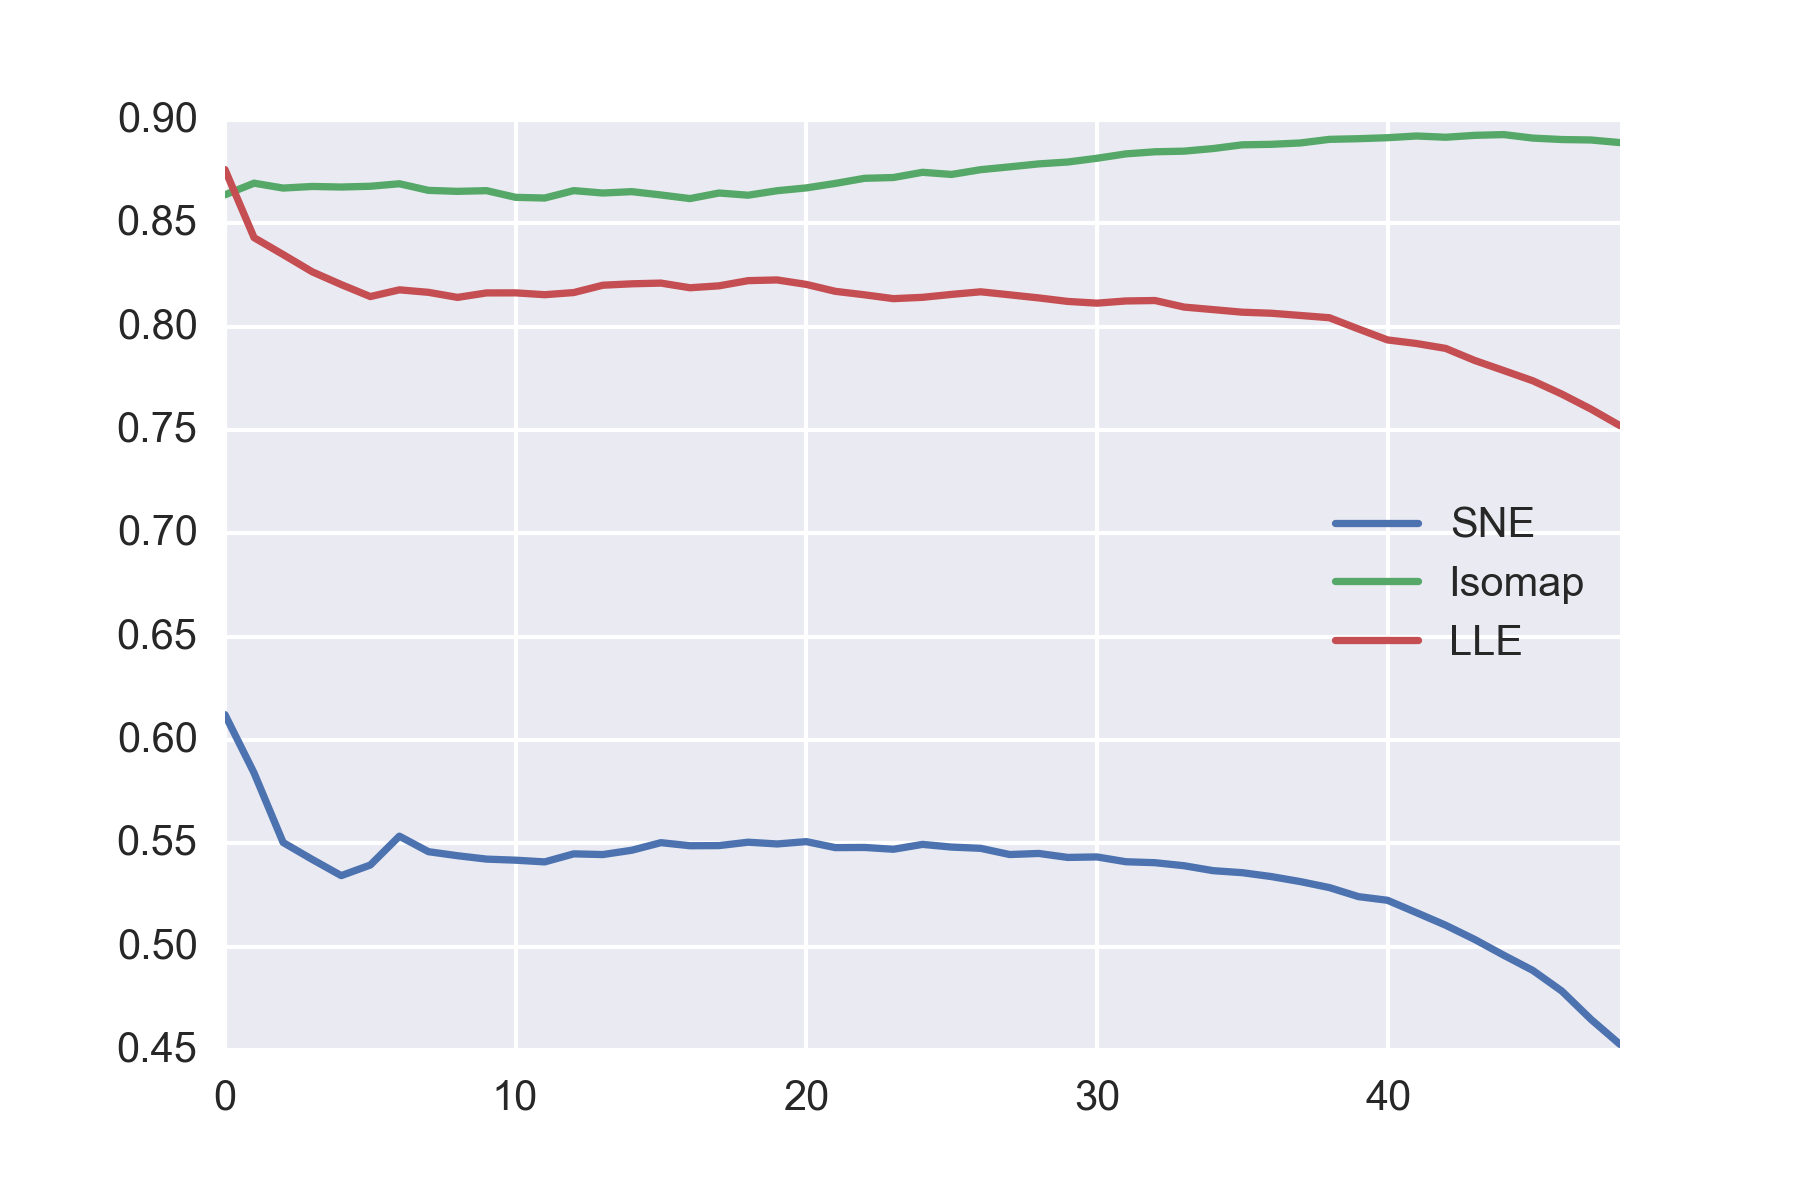
\includegraphics[width=0.49\textwidth]{figures/quality_measures/line_trustworthiness_3d.png}}
	\subfigure{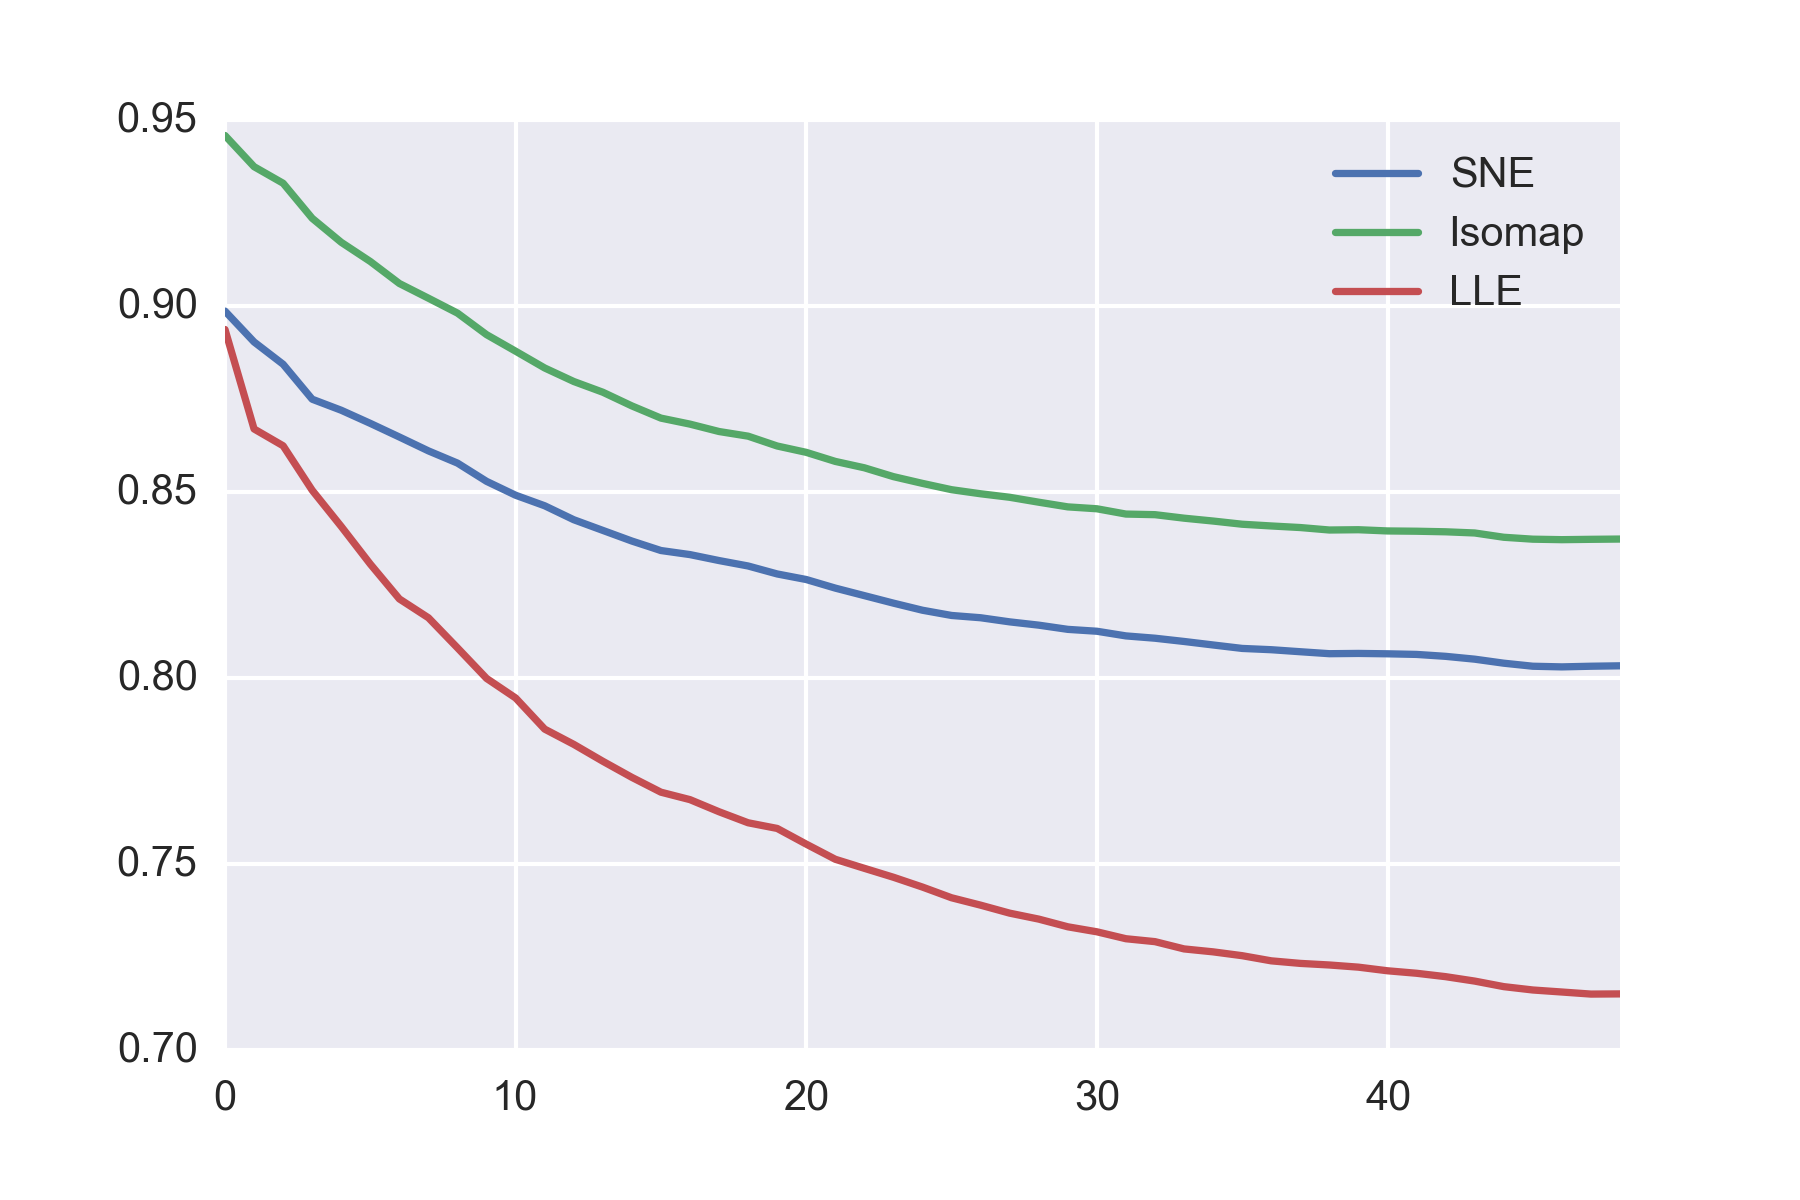
\includegraphics[width=0.49\textwidth]{figures/quality_measures/line_continuity_3d.png}}
	\caption{Trustworthiness (left) and continuity (right) of the 3D projections produced from line features.}\label{fig:TC_3d_lines}
\end{figure}

\begin{figure}[H]
	\centering
	\subfigure{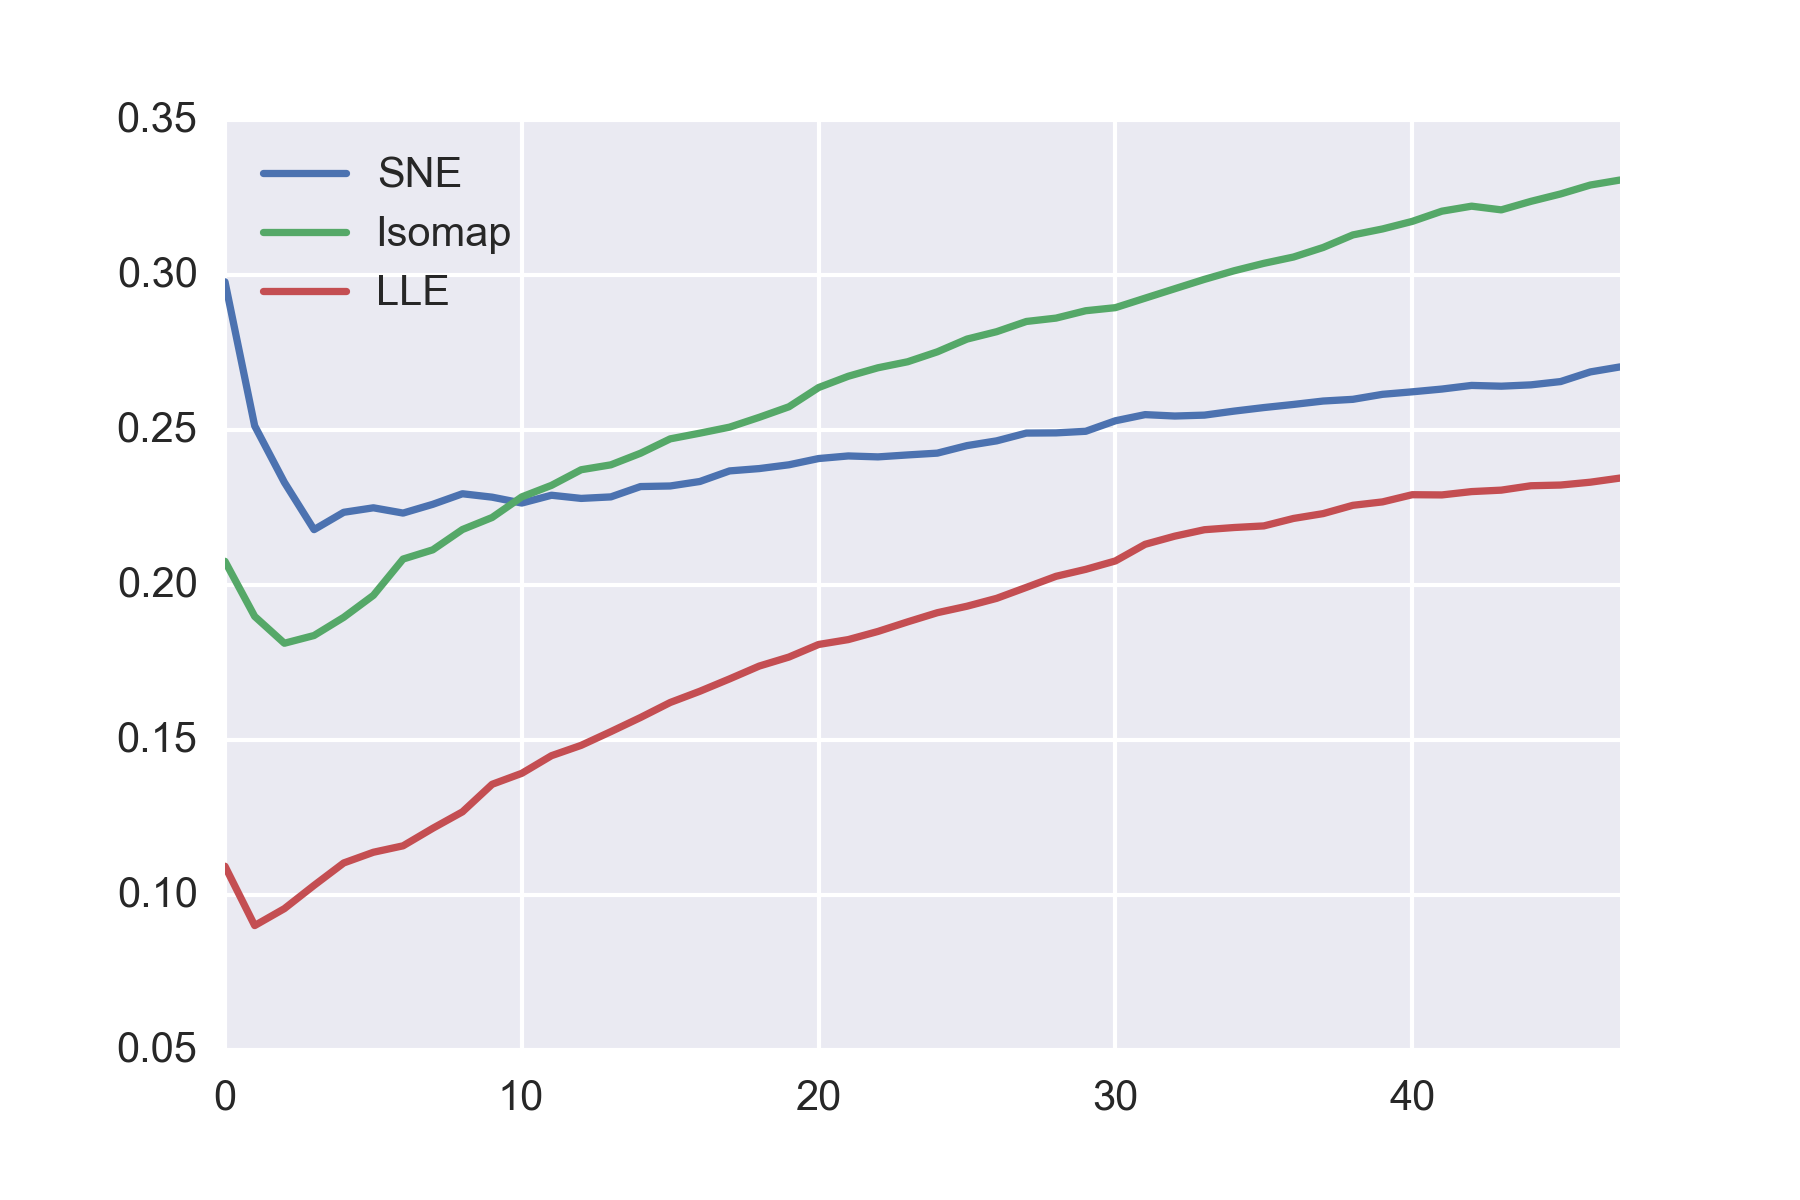
\includegraphics[width=0.49\textwidth]{figures/quality_measures/line_lcmc_2d.png}}
	\subfigure{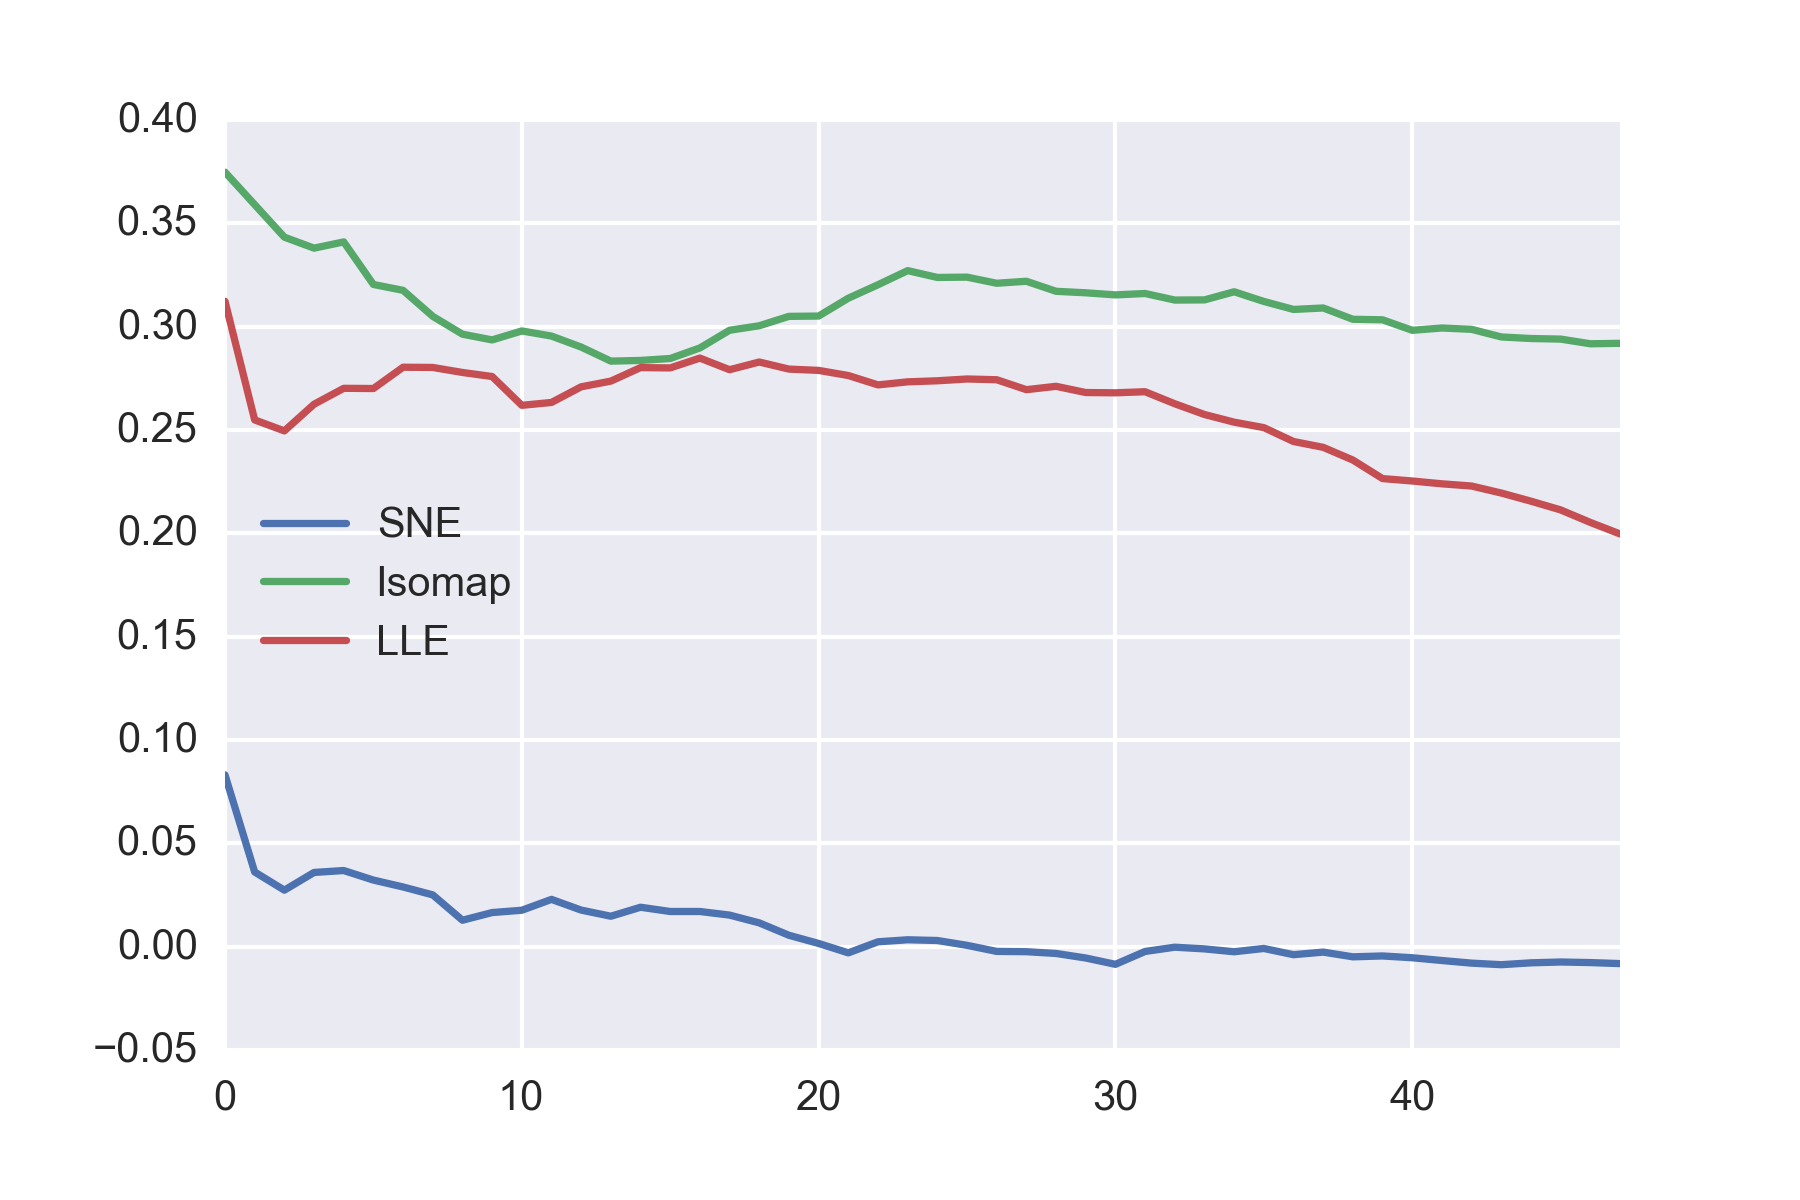
\includegraphics[width=0.49\textwidth]{figures/quality_measures/line_lcmc_3d.png}}
	\caption{LCMC of both the 2D projection (left) and 3D projection (right) of the feature space for lines.}\label{fig:LCMC_lines}
\end{figure}
\clearpage

\subsection{Intensity \& Texture Features}
\label{subsec:results-texture}
Intensity and texture features showed the lowest similarity between the real and phantom datasets. As can be seen in figure \ref{fig:mammogram-histogram} the intensity distribution of the phantom mammograms are nothing like a real mammogram. Because of this difference the results show that the they are clearly in different spaces. The results of the KS two sample test showed that the two distributions generated for both intensity and texture features are completely different. The results of the two sample Kolmogorov-Smirnov test are included in appendix \ref{appendix:ks-test} because the number of features for blobs is based on the number of scales used leading to the a large number (up to 100) of entries. 

The feature spaces presented in this section were generated by taking ROIs defined by the blob and line features detected from each of the mammograms by computing intensity and texture features from each image patch. Because blobs are detected across a range of scales the average value for each scale is used leading to a feature space of size $nk$ where $n$ is the number of features and $k$ is the number of scales (e.g. for texture: $n = 4$ and $k = 10$ so it has $40$ features). 

The results of performing dimensionality reduction on both of these feature spaces is that in all cases the synthetic mammograms are separated from the real mammograms into an isolated cluster on their own. This is because the values for both types of feature are on average much higher for the breast phantoms than the real mammograms.

For features derived from patches defined by blobs it can be seen that between the real mammograms there is a trend visible in both intensity and textural features which causes some transition between high to low risk. This is particularly visible for intensity features in the 2D plot produced by t-SNE shown in figure \ref{fig:intensity_SNE_mapping} and in the 2D plot in figure \ref{fig:texture_SNE_mapping} for texture features. 

In the case of intensity features this transition is caused by blobs which are of higher intensity. For texture features the trend is explained by a transition for blobs with low contrast and dissimilarity and high homogeneity and energy corresponding to high risk blobs transitioning through to low risk blobs where the reverse is true.

Intensity features derived from lines do show a degree of separation between high and low risk mammograms. High risk mammograms typically have a higher average intensity. This is most clearly seen in the 2D visualisations produced by t-SNE and Isomap in \ref{fig:intensity_SNE_mapping_lines} and \ref{fig:intensity_iso_mapping_lines}. On the other hand the texture features do not appear to show any meaningful relationship between risk classes.

The quality measures for intensity features derived from blobs show that t-SNE produces the best visualisation in two dimensions but is again beaten by Isomap in three dimensions for anything larger than a small local neighbourhood. For texture features Isomap appears to out do t-SNE in all measures for neighbourhoods larger than 10.

Quality measures taken from the visualisations for intensity from lines show again that t-SNE is best for small values of $k$ in both 2 and 3 dimensions but is overtaken by Isomap and LLE for neighbourhoods of larger sizes. The results are similar for texture features derived from lines but in this case the performance of t-SNE is only very marginally better for small values of $k$. In almost all cases for texture from lines Isomap quickly overtakes t-SNE as having higher or similar quality projections.

%------------------------------------------------------------------------------------
% Blob intensity and texture features
%------------------------------------------------------------------------------------

\begin{figure}[H]
	\label{fig:mammogram-histogram}
	\centering
	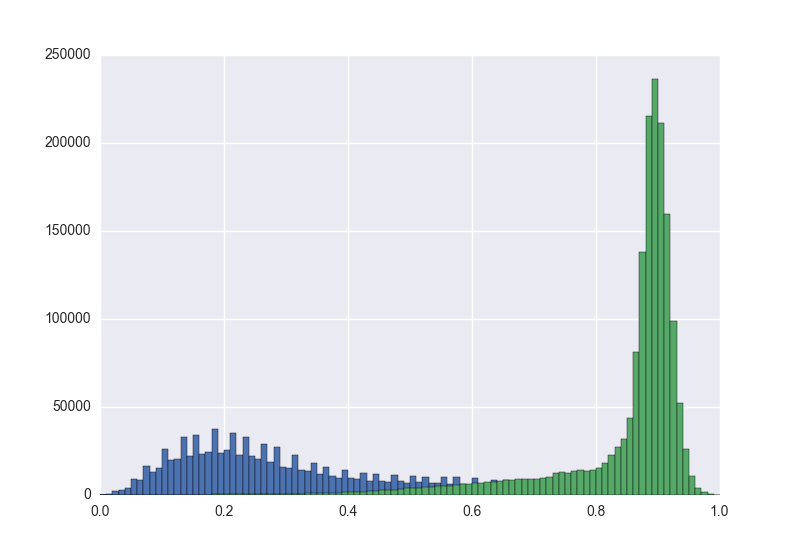
\includegraphics[width=0.8\textwidth]{Images/inverted_hist.png}	
	\caption{Comparison of the histogram of a real mammogram (blue) against a synthetic mammogram (green). The distribution of intensities are radically different from one another.}
\end{figure}

\clearpage
\begin{figure}[H]
	\centering
	\subfigure{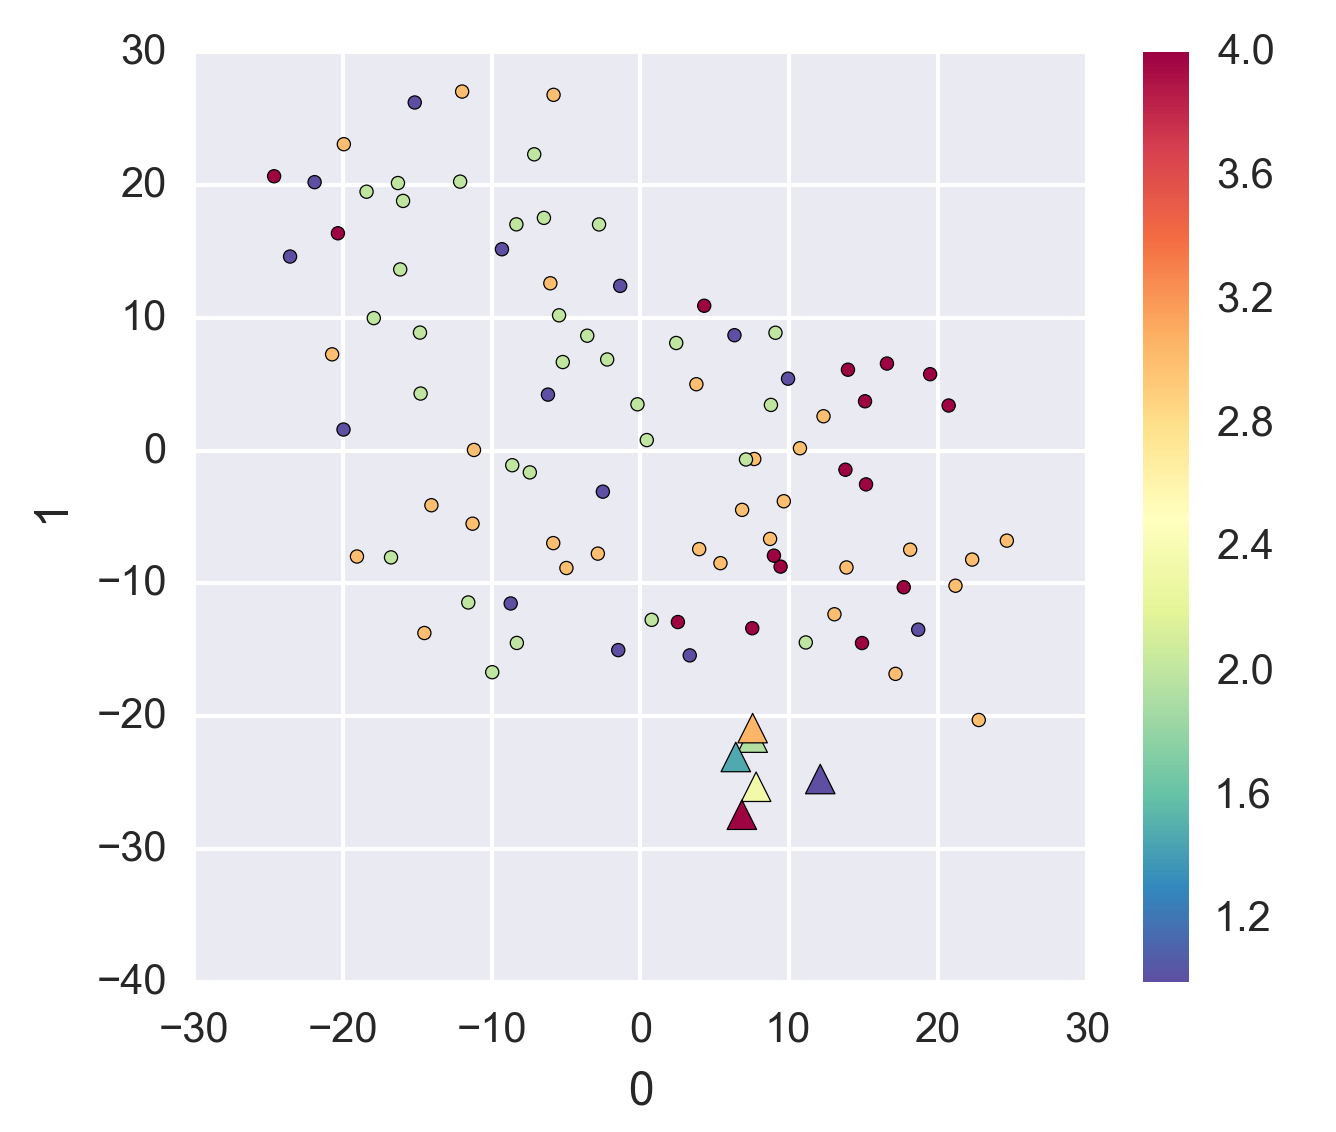
\includegraphics[width=0.49\textwidth]{figures/mappings/intensity_SNE_mapping_2d.png}}
	\subfigure{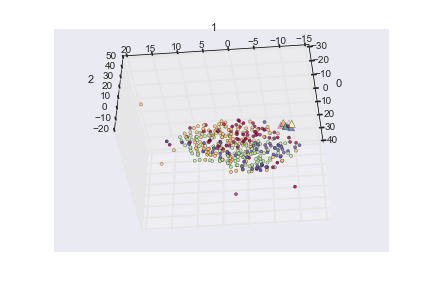
\includegraphics[width=0.49\textwidth]{figures/mappings/intensity_SNE_mapping_3d.png}}
	\caption{2D \& 3D projections of the intensity feature space produced by the t-SNE algorithm with a learning rate of 300 and perplexity of 30.}\label{fig:intensity_SNE_mapping}
\end{figure}

\begin{figure}[H]
	\centering
	\subfigure{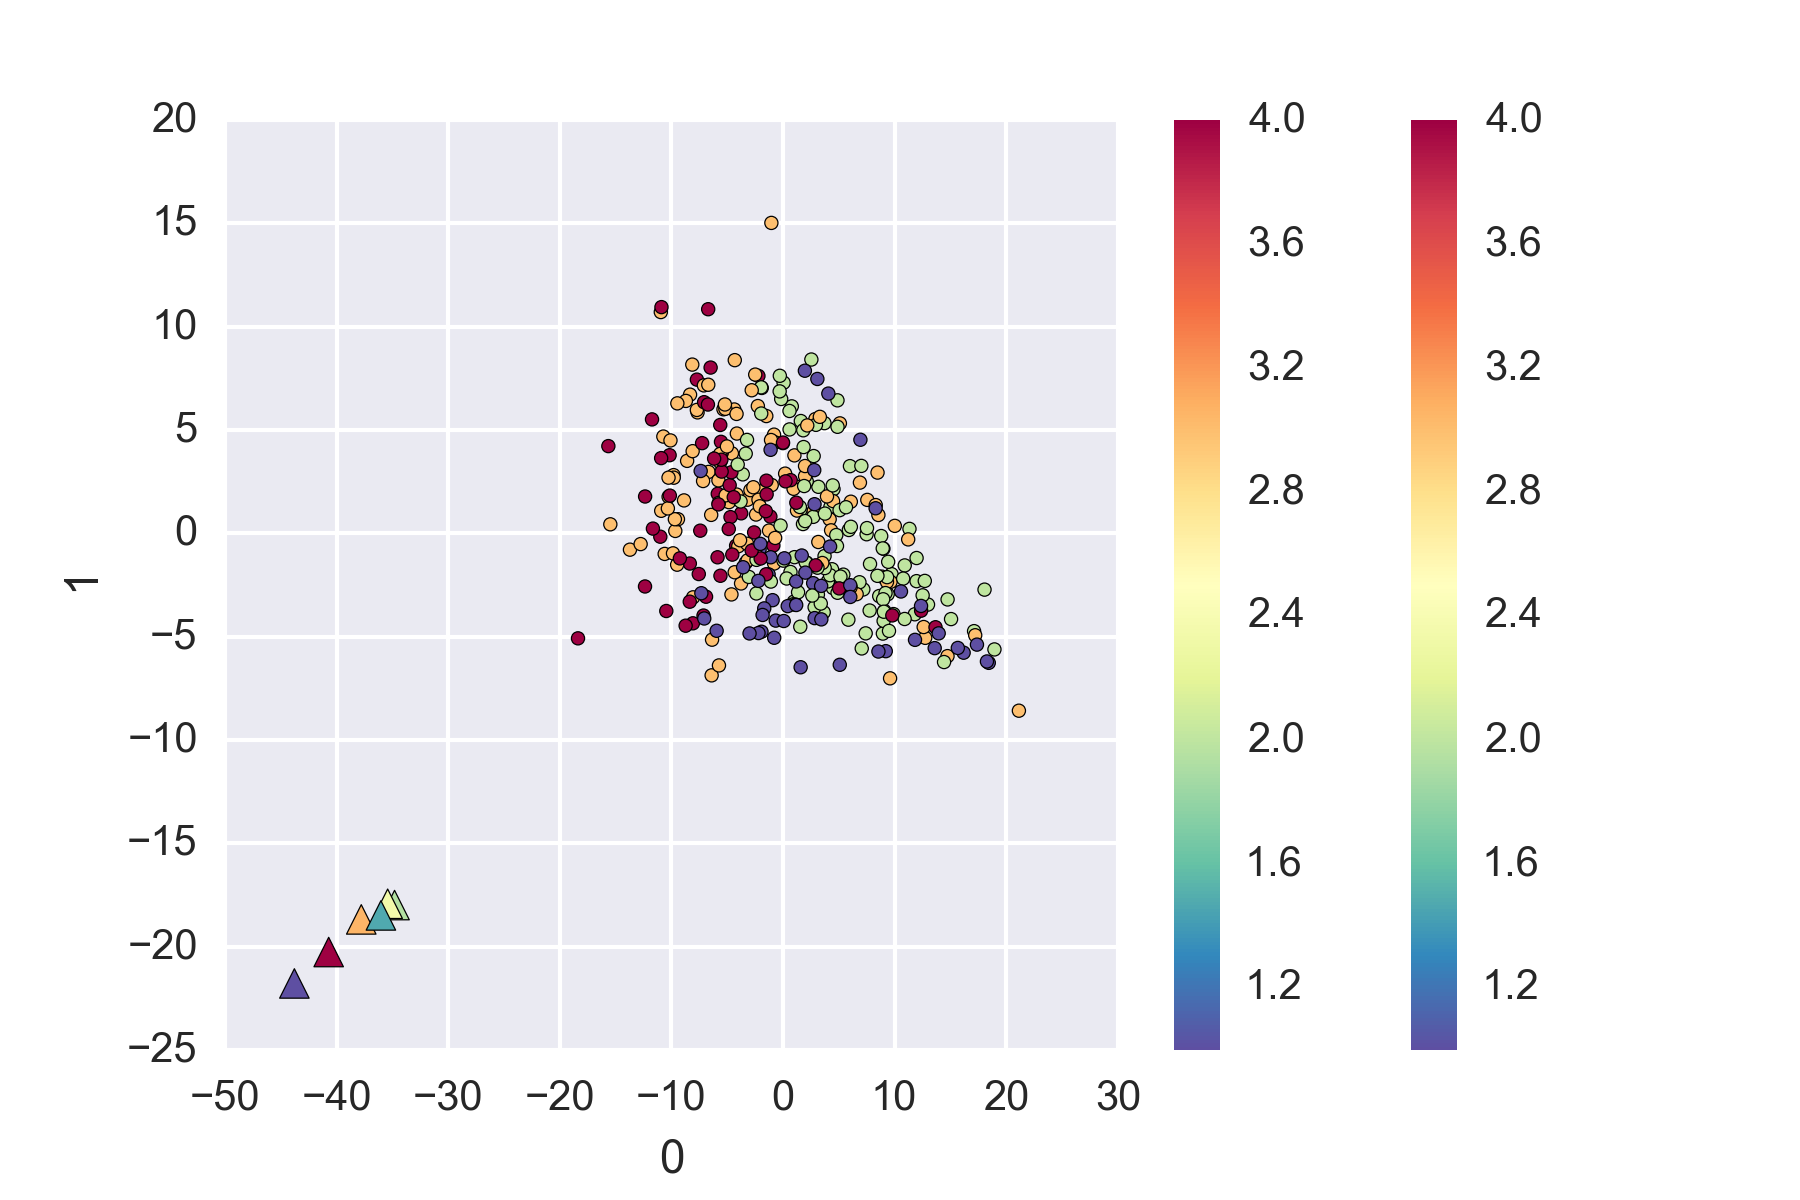
\includegraphics[width=0.49\textwidth]{figures/mappings/intensity_iso_mapping_2d.png}}
	\subfigure{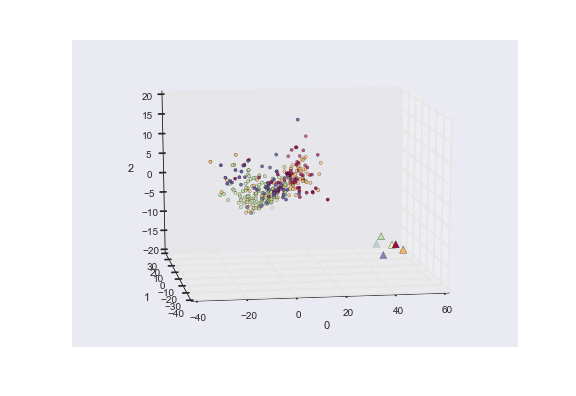
\includegraphics[width=0.49\textwidth]{figures/mappings/intensity_iso_mapping_3d.png}}
	\caption{2D \& 3D projections of the intensity feature space generated from blobs produced by the Isomap algorithm with 50 neighbours.}\label{fig:intensity_iso_mapping}
\end{figure}

\begin{figure}[H]
	\centering
	\subfigure{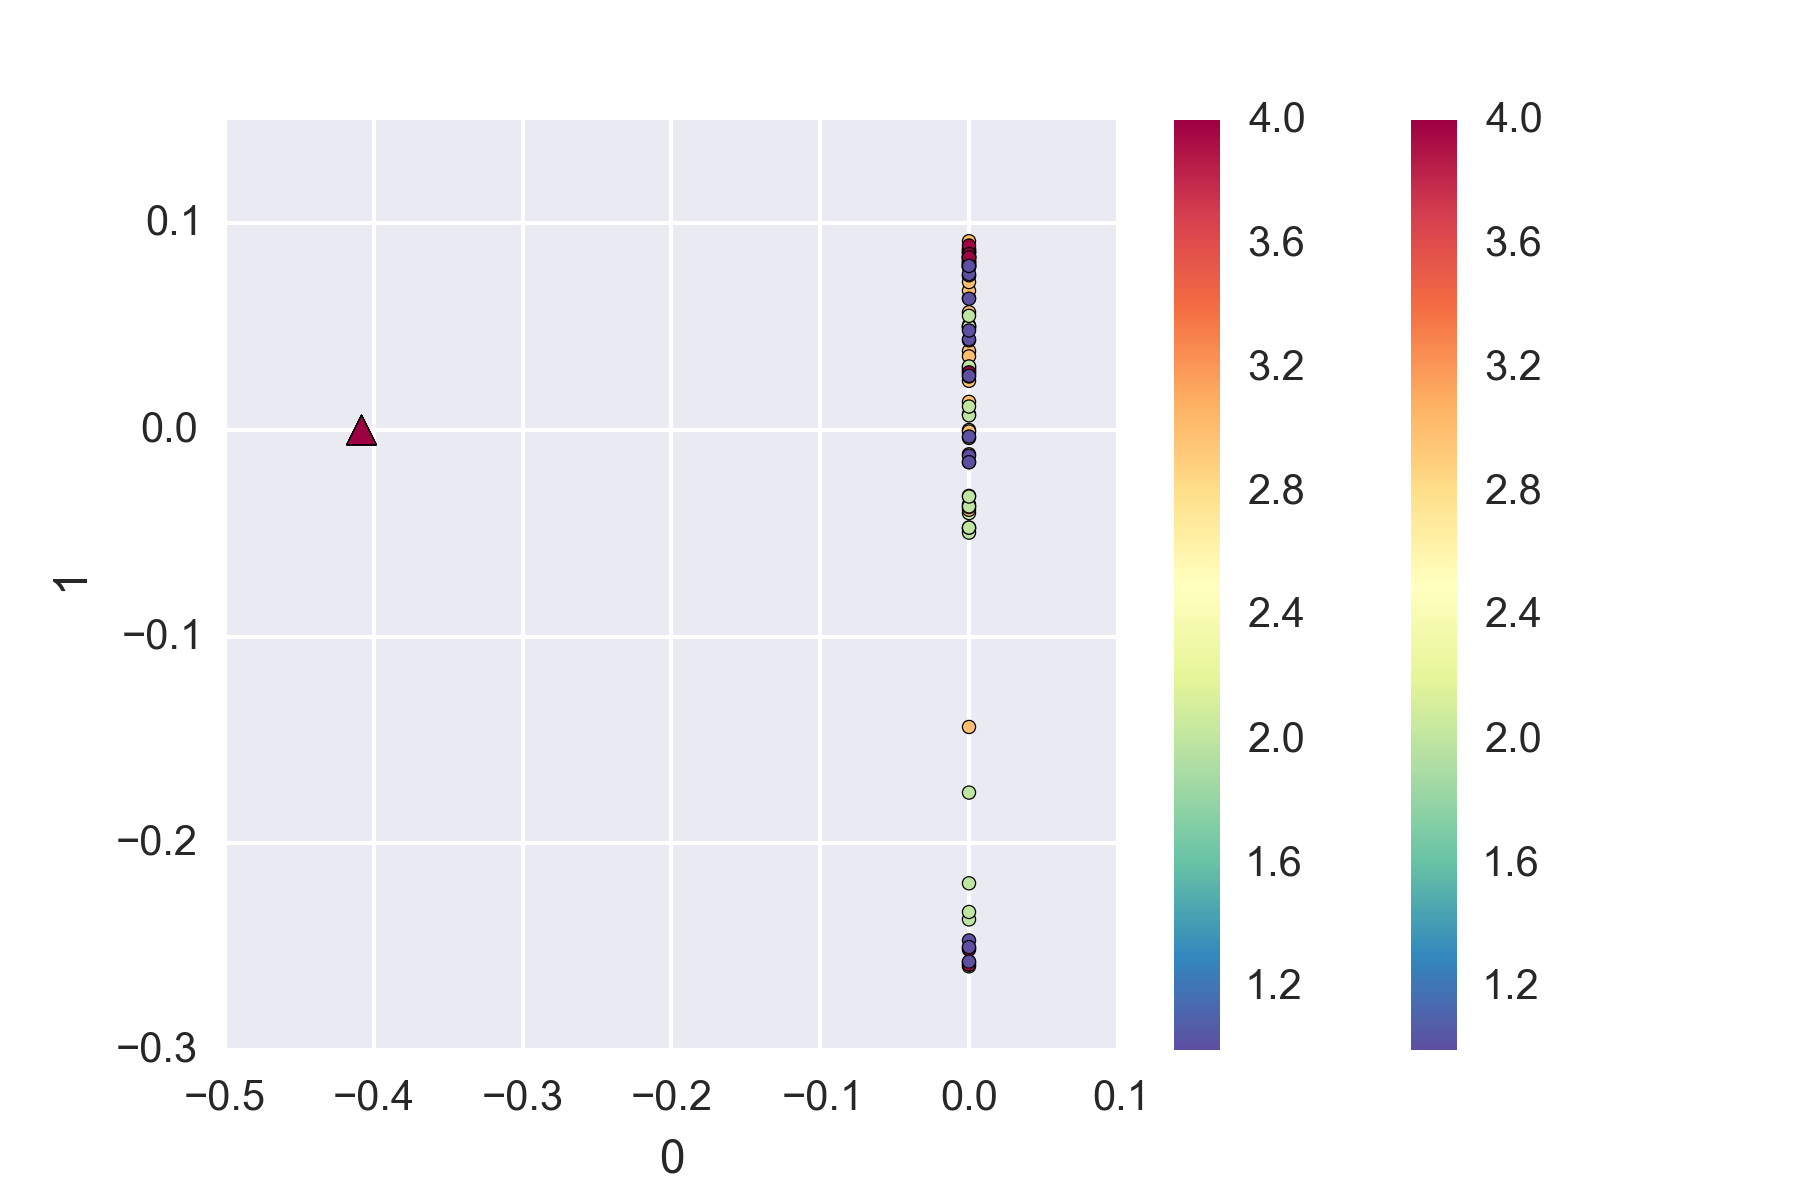
\includegraphics[width=0.49\textwidth]{figures/mappings/intensity_lle_mapping_2d.png}}
	\subfigure{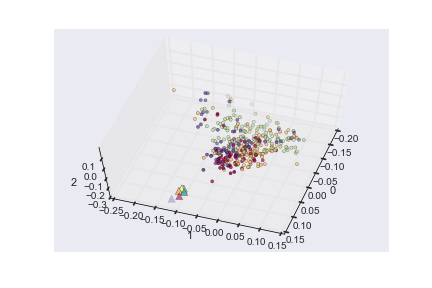
\includegraphics[width=0.49\textwidth]{figures/mappings/intensity_lle_mapping_3d.png}}
	\caption{2D \& 3D projections of the intensity feature space generated from blobs produced by the LLE algorithm with 50 neighbours.}\label{fig:intensity_LLE_mapping}
\end{figure}
\clearpage

% Quality for blob intensity features
%------------------------------------------------------------------------------------
\clearpage
\begin{figure}[H]
	\centering
	\subfigure{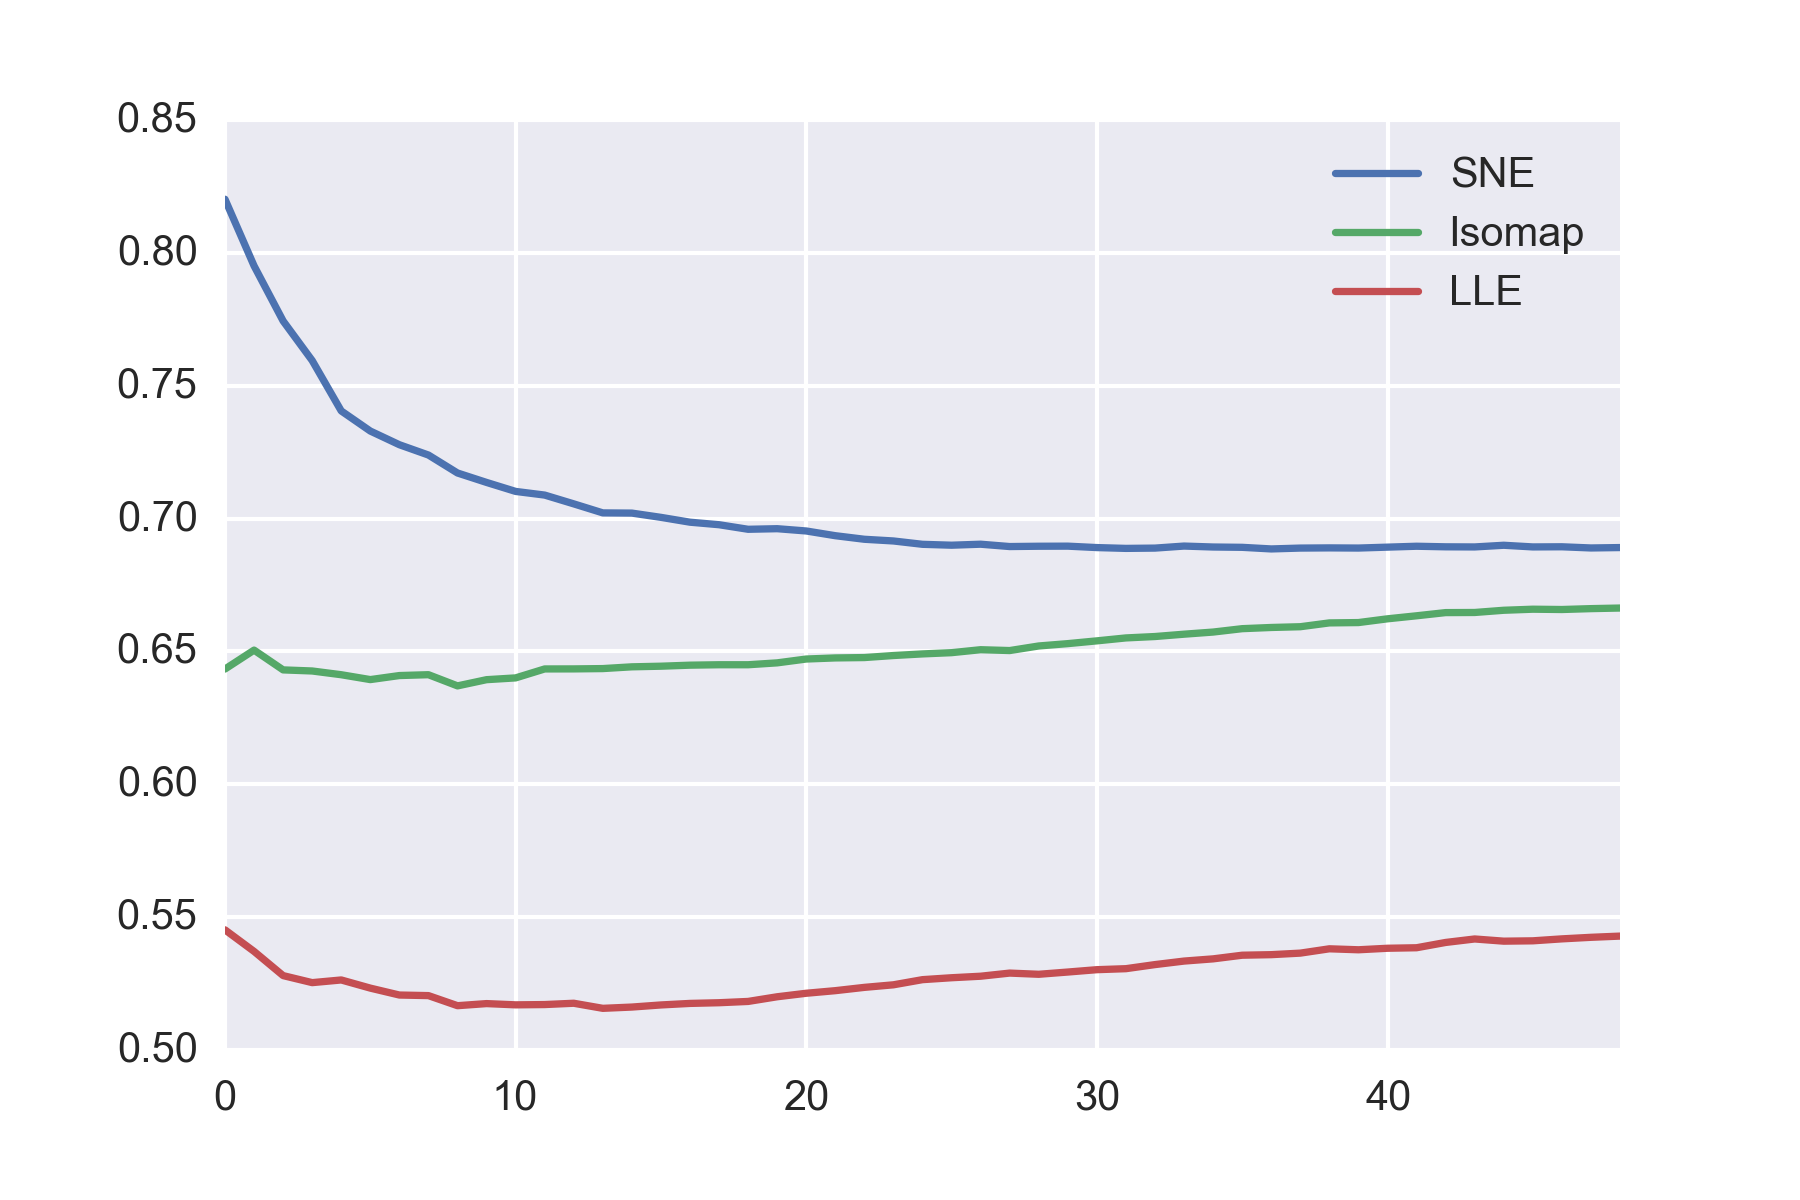
\includegraphics[width=0.49\textwidth]{figures/quality_measures/intensity_trustworthiness_2d.png}}
	\subfigure{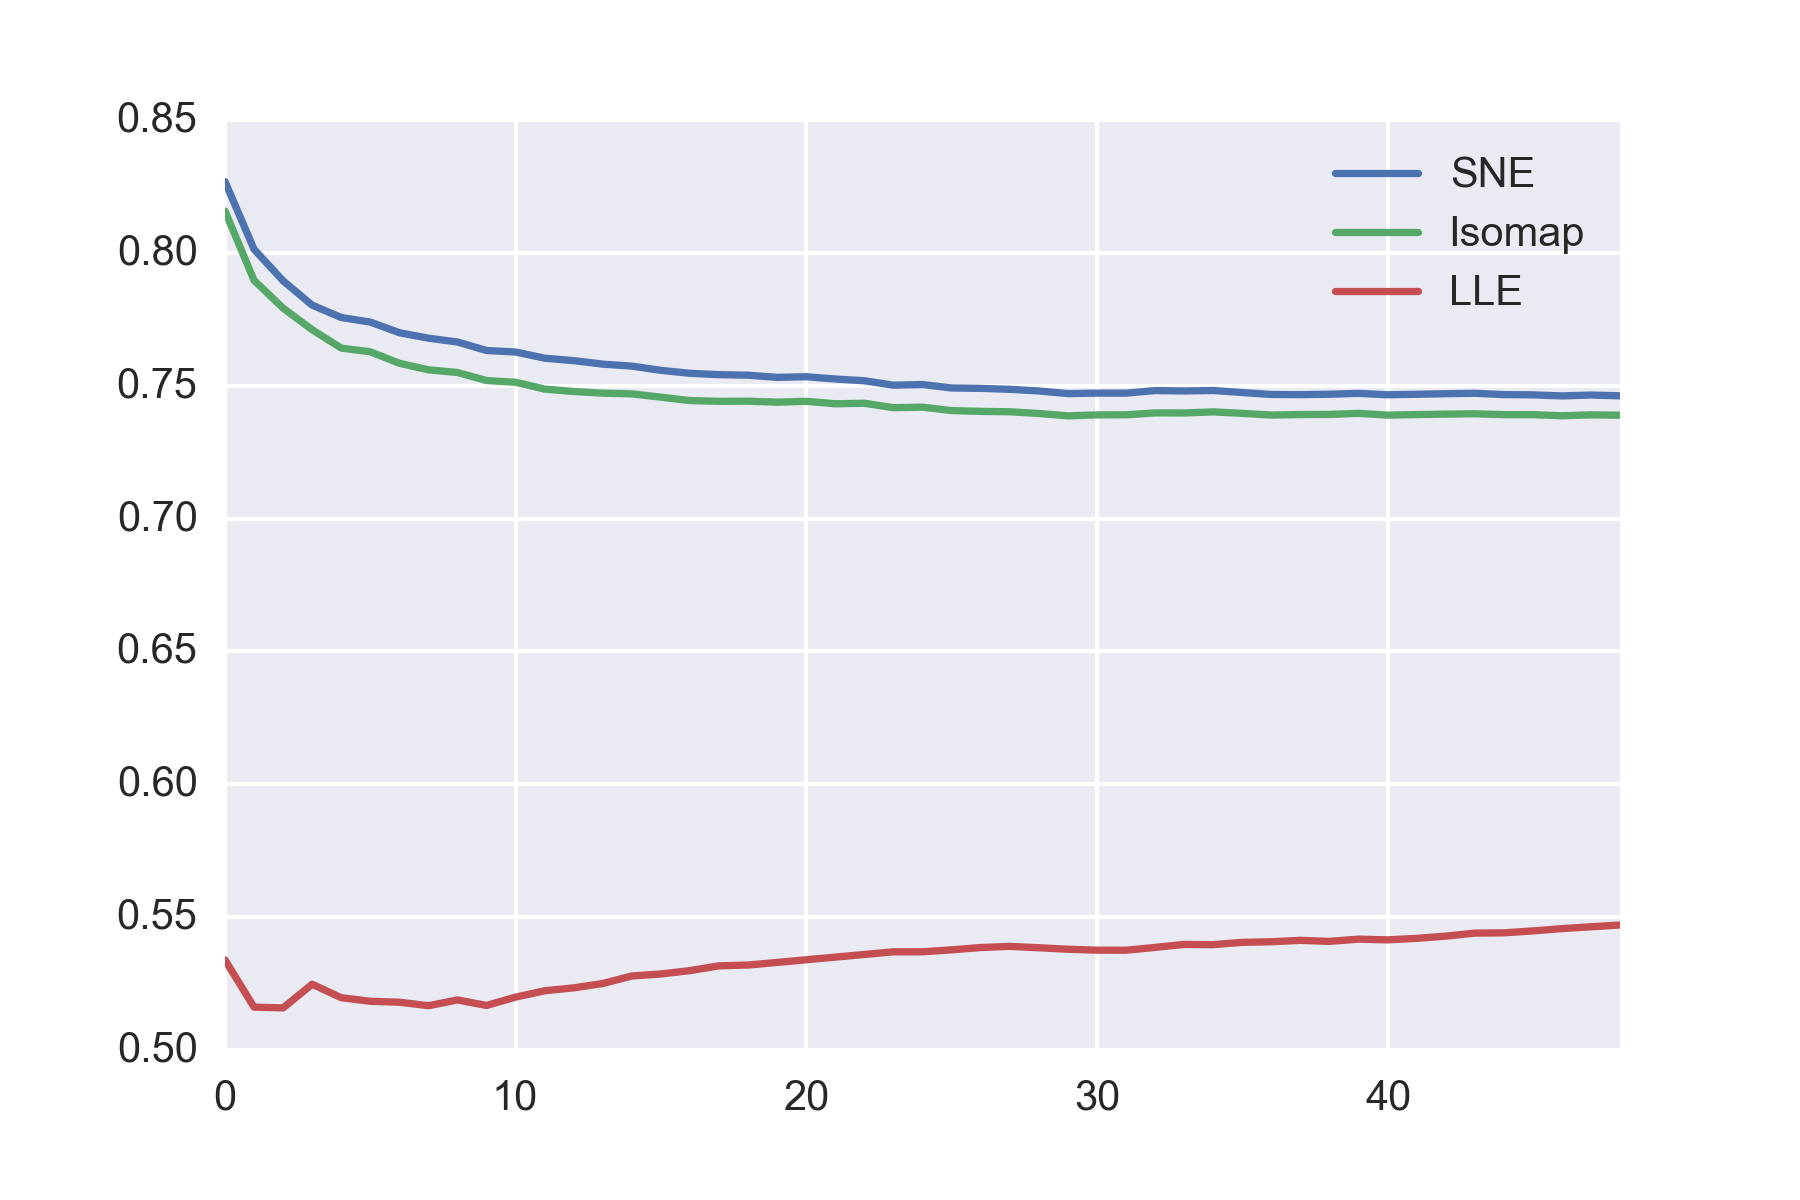
\includegraphics[width=0.49\textwidth]{figures/quality_measures/intensity_continuity_2d.png}}
	\caption{Trustworthiness (left) and continuity (right) of the 2D projections produced from intensity features from blobs.}\label{fig:TC_2d_intensity}
\end{figure}

\begin{figure}[H]
	\centering
	\subfigure{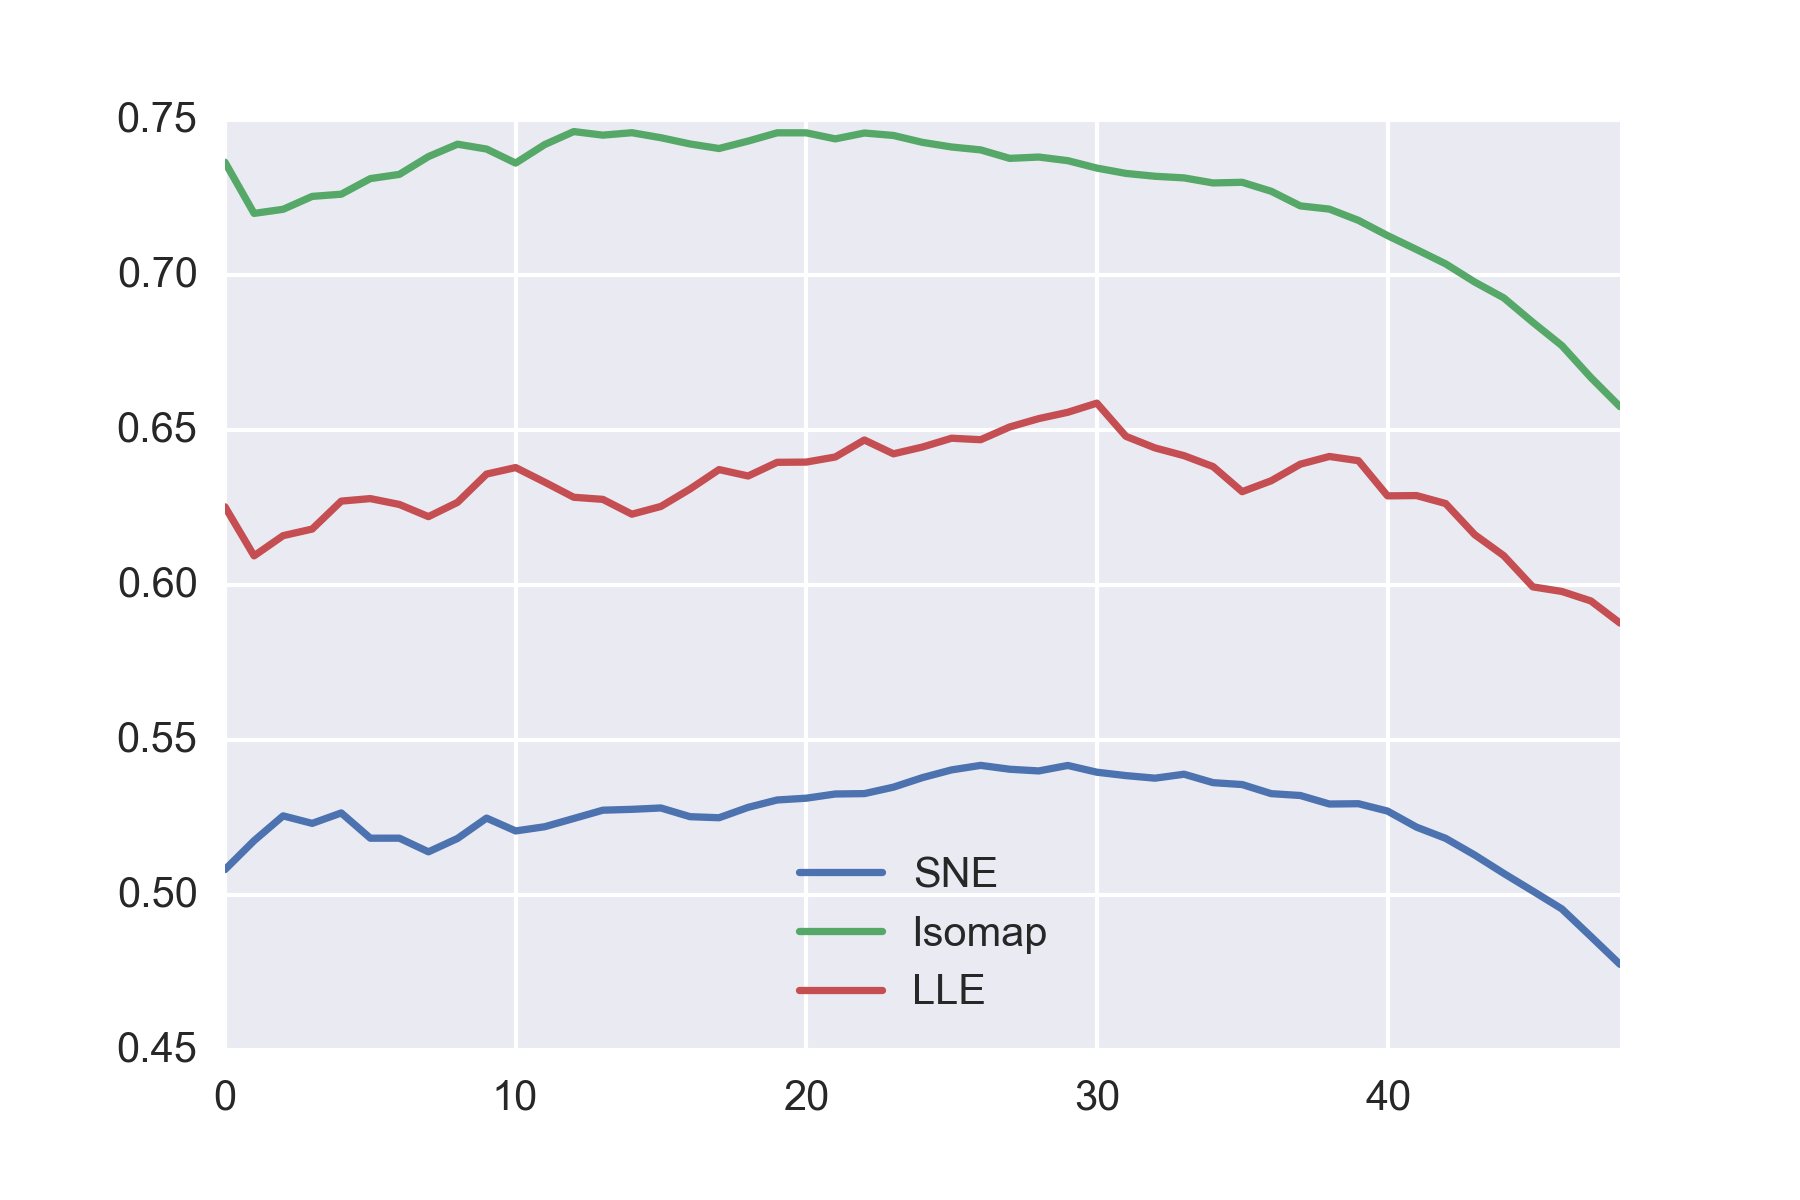
\includegraphics[width=0.49\textwidth]{figures/quality_measures/intensity_trustworthiness_3d.png}}
	\subfigure{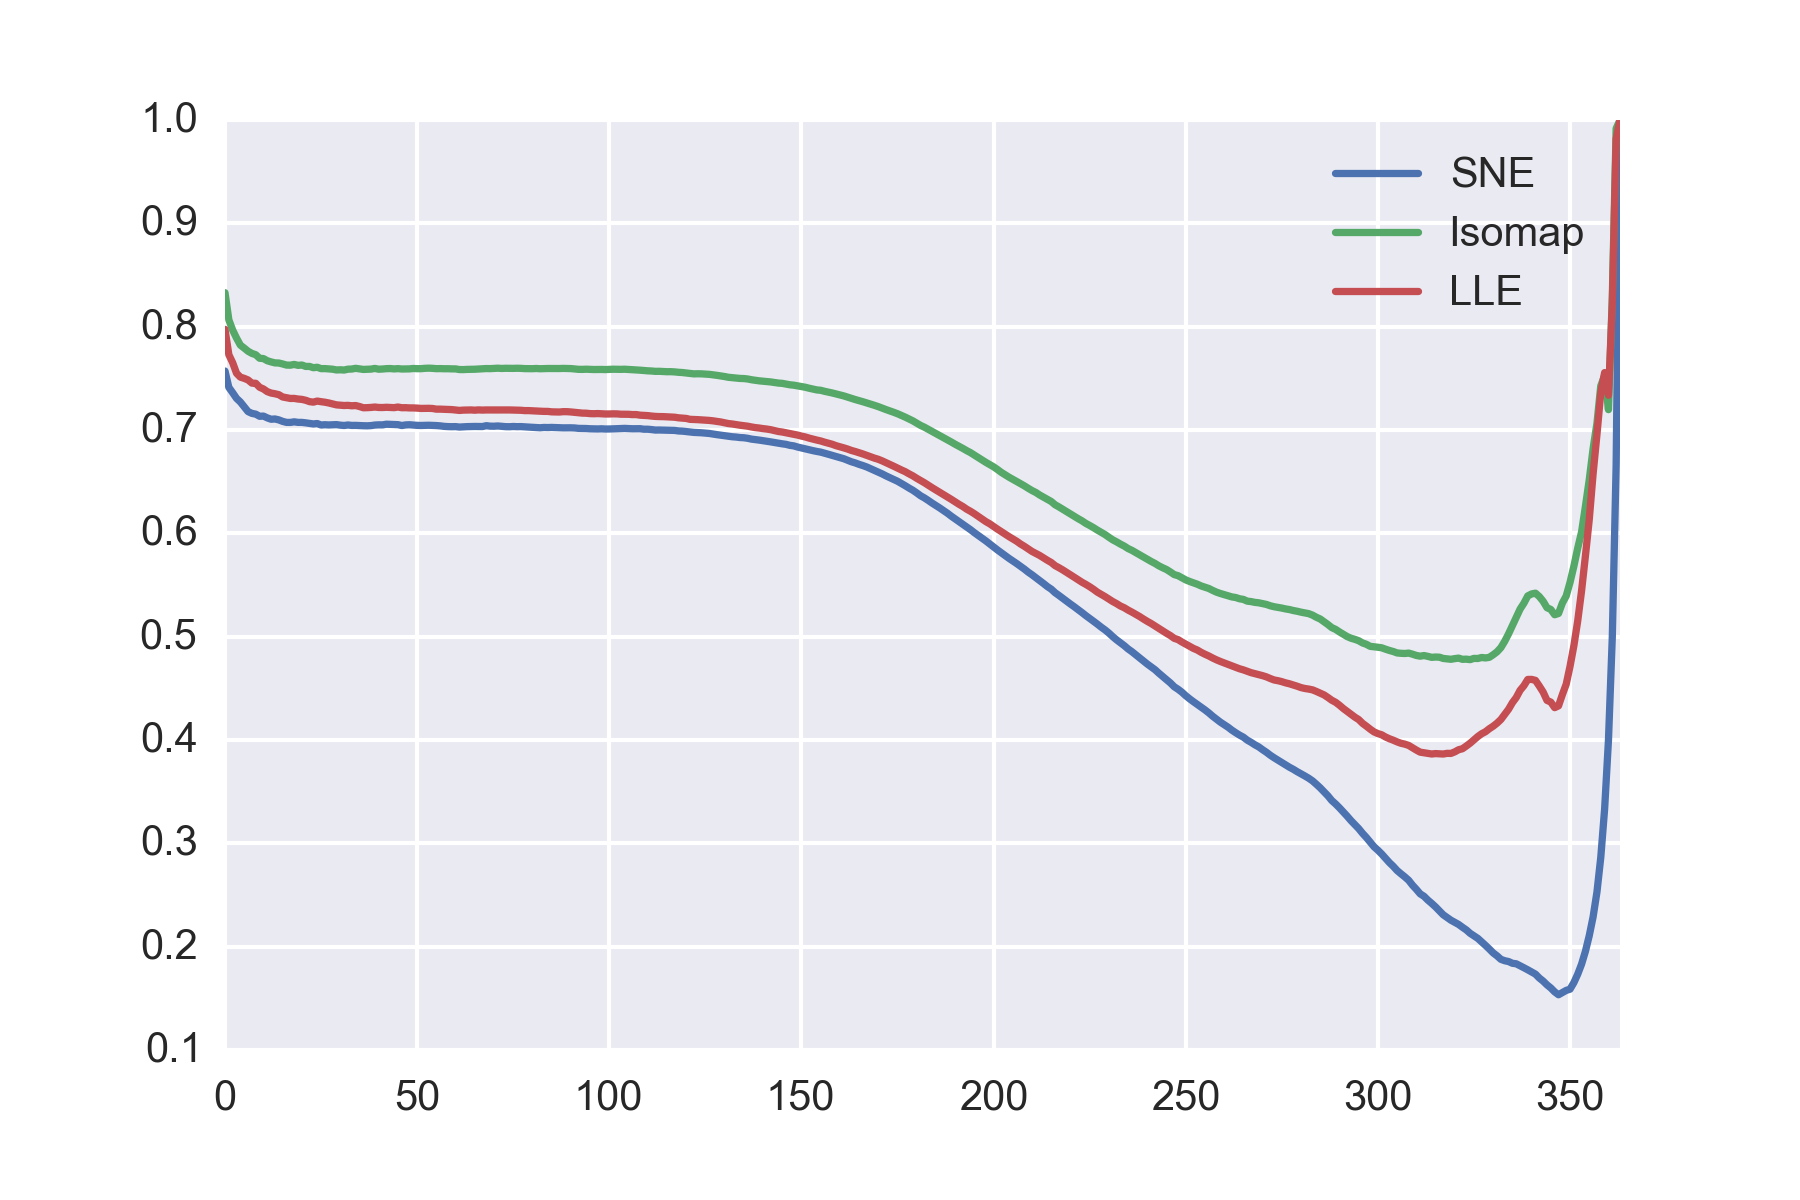
\includegraphics[width=0.49\textwidth]{figures/quality_measures/intensity_continuity_3d.png}}
	\caption{Trustworthiness (left) and continuity (right) of the 3D projections produced from intensity features from blobs.}\label{fig:TC_3d_intensity}
\end{figure}

\begin{figure}[H]
	\centering
	\subfigure{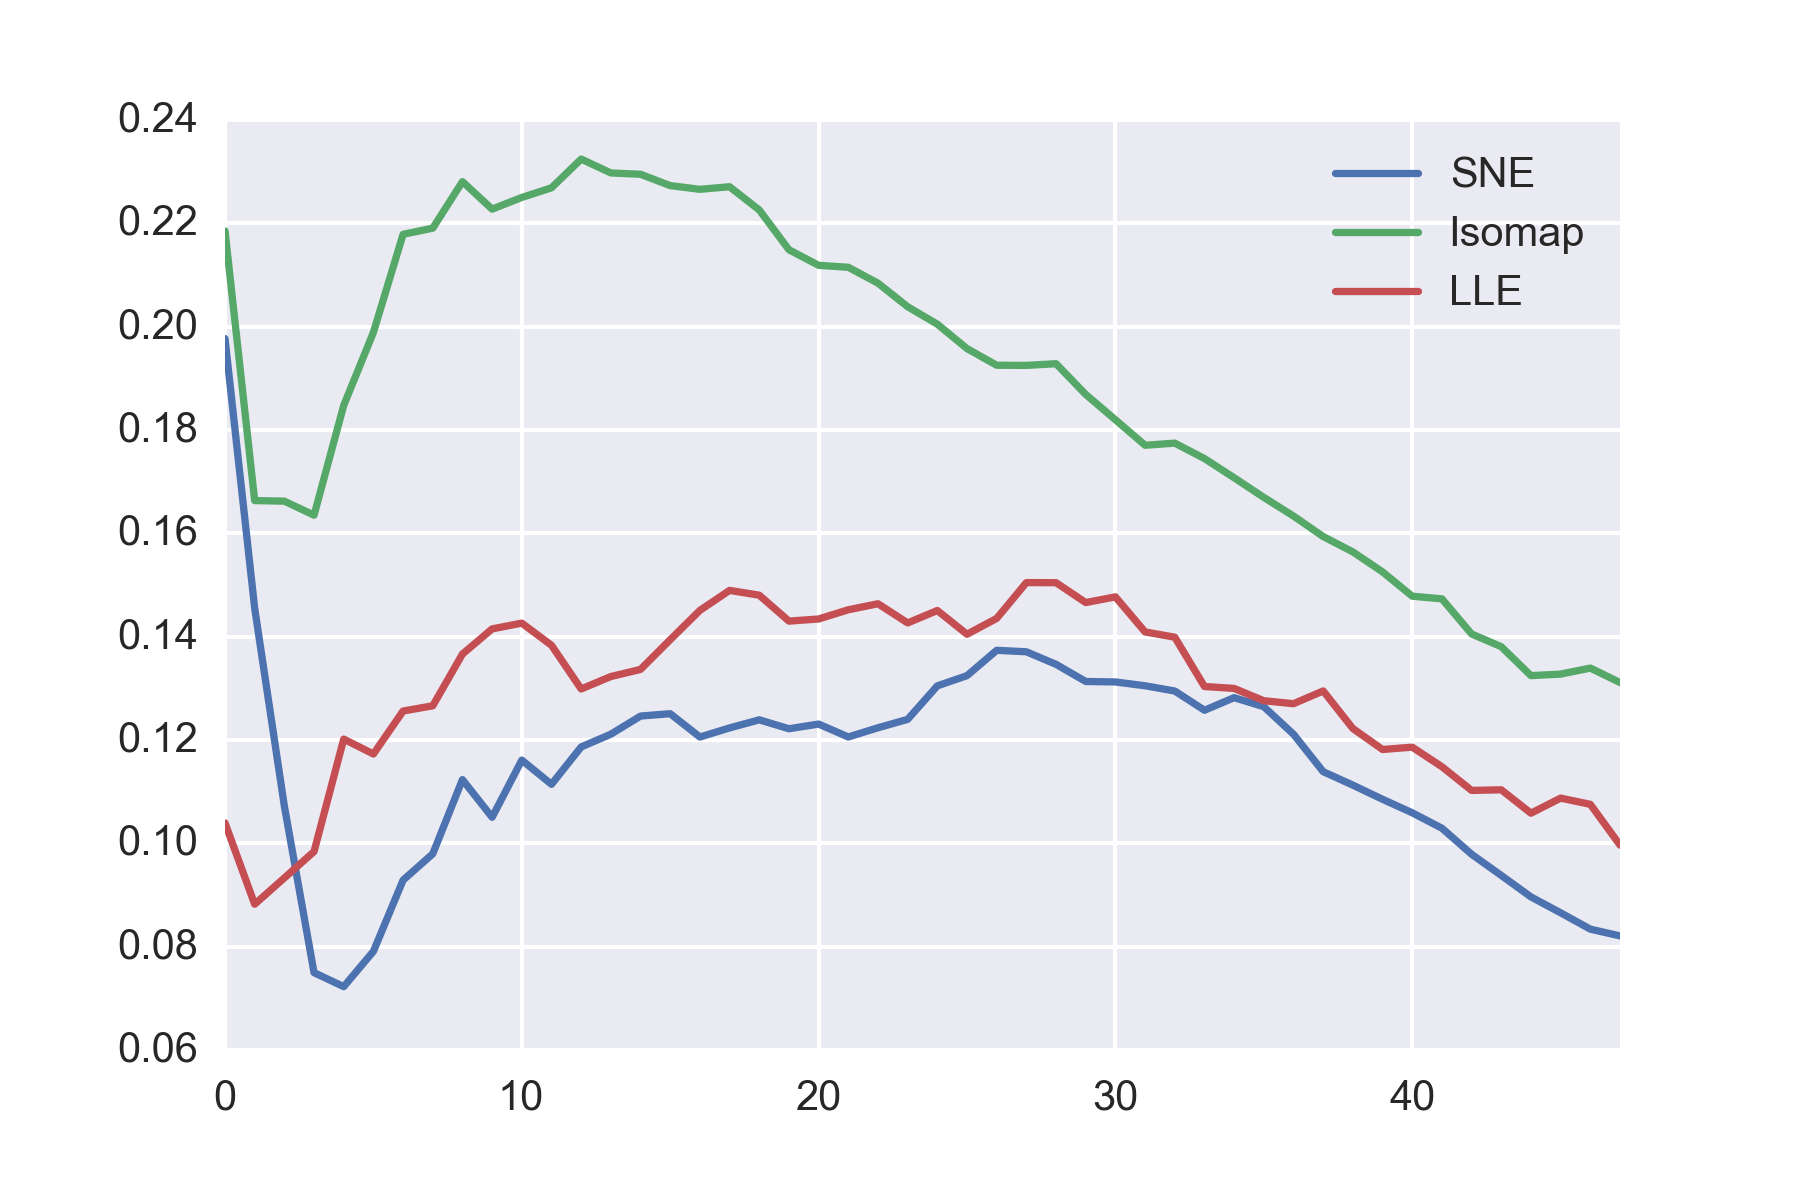
\includegraphics[width=0.49\textwidth]{figures/quality_measures/intensity_lcmc_2d.png}}
	\subfigure{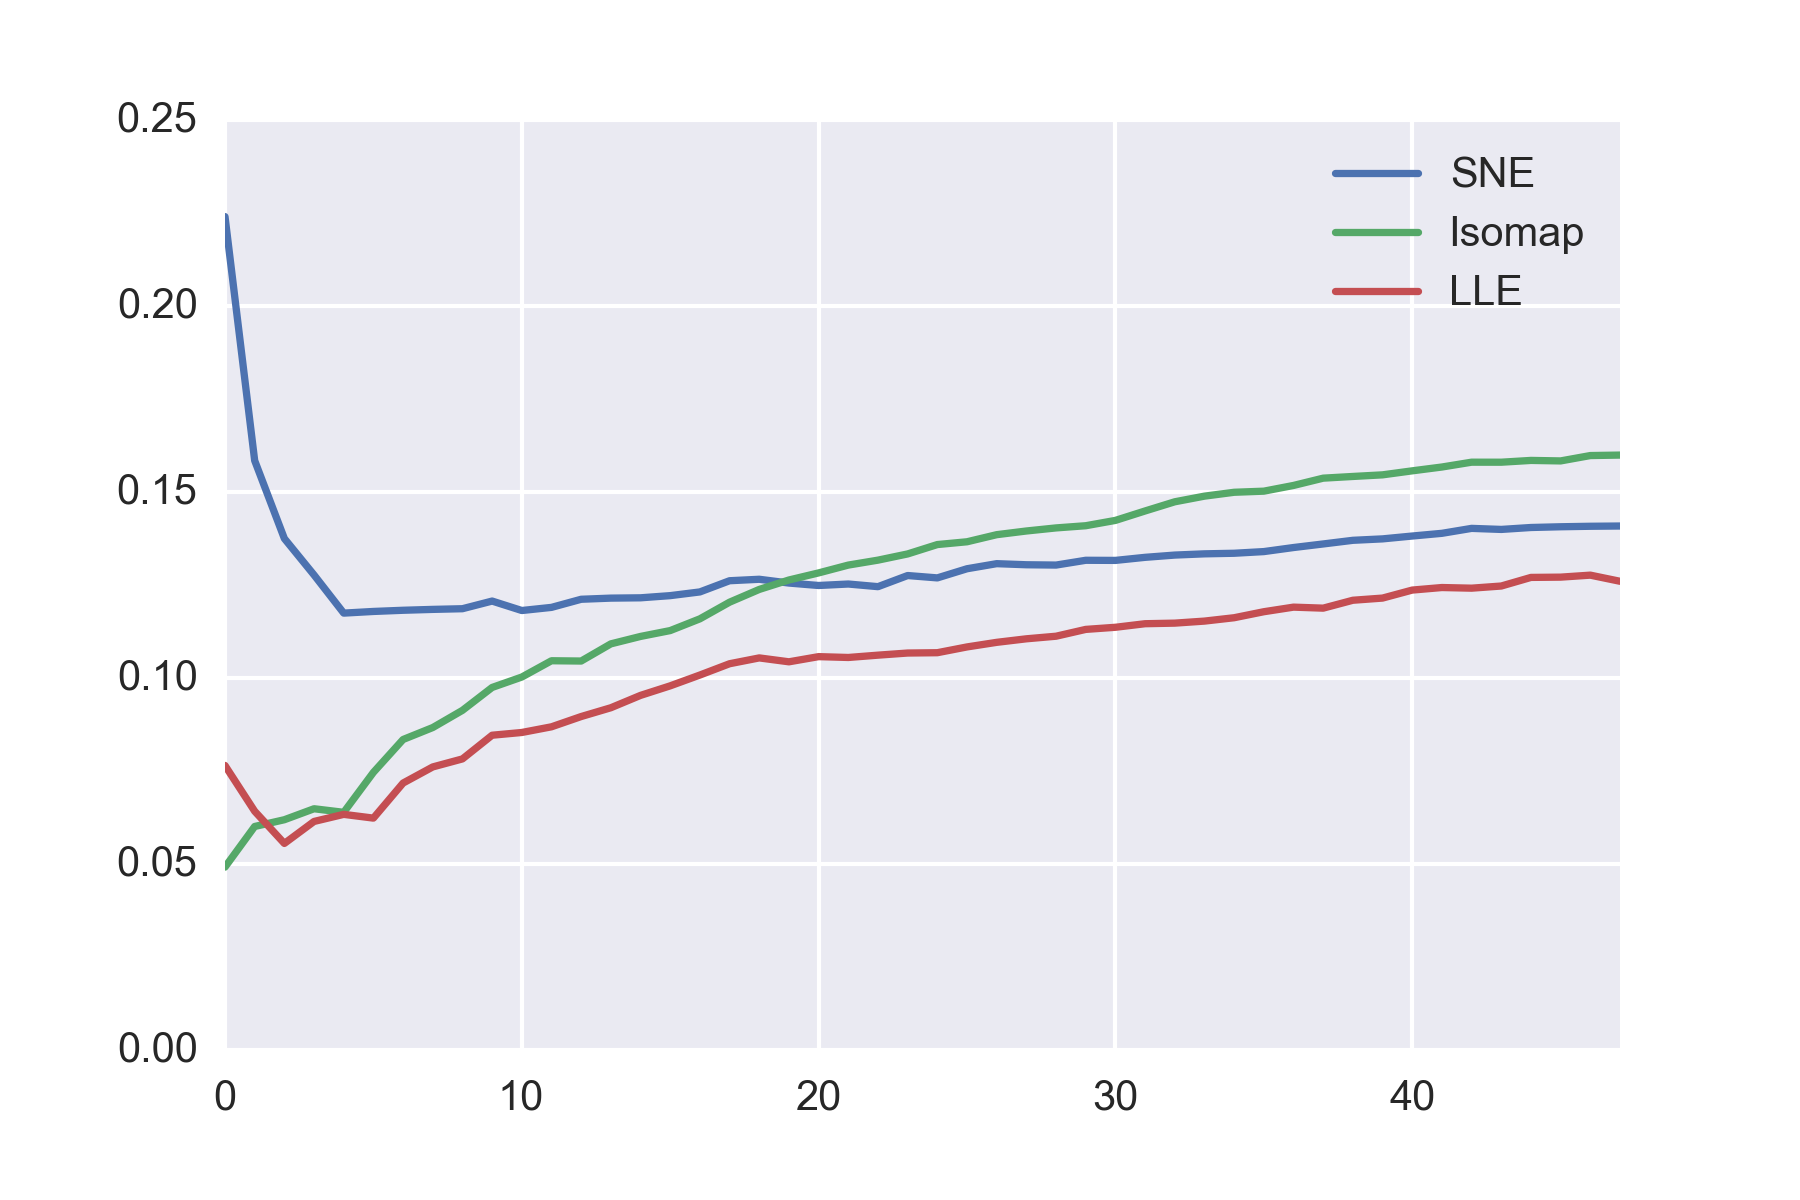
\includegraphics[width=0.49\textwidth]{figures/quality_measures/intensity_lcmc_3d.png}}
	\caption{LCMC of both the 2D projection (left) and 3D projection (right) of the feature space for intensity from blobs.}\label{fig:LCMC_intensity}
\end{figure}
\clearpage

\clearpage
\begin{figure}[H]
	\centering
	\subfigure{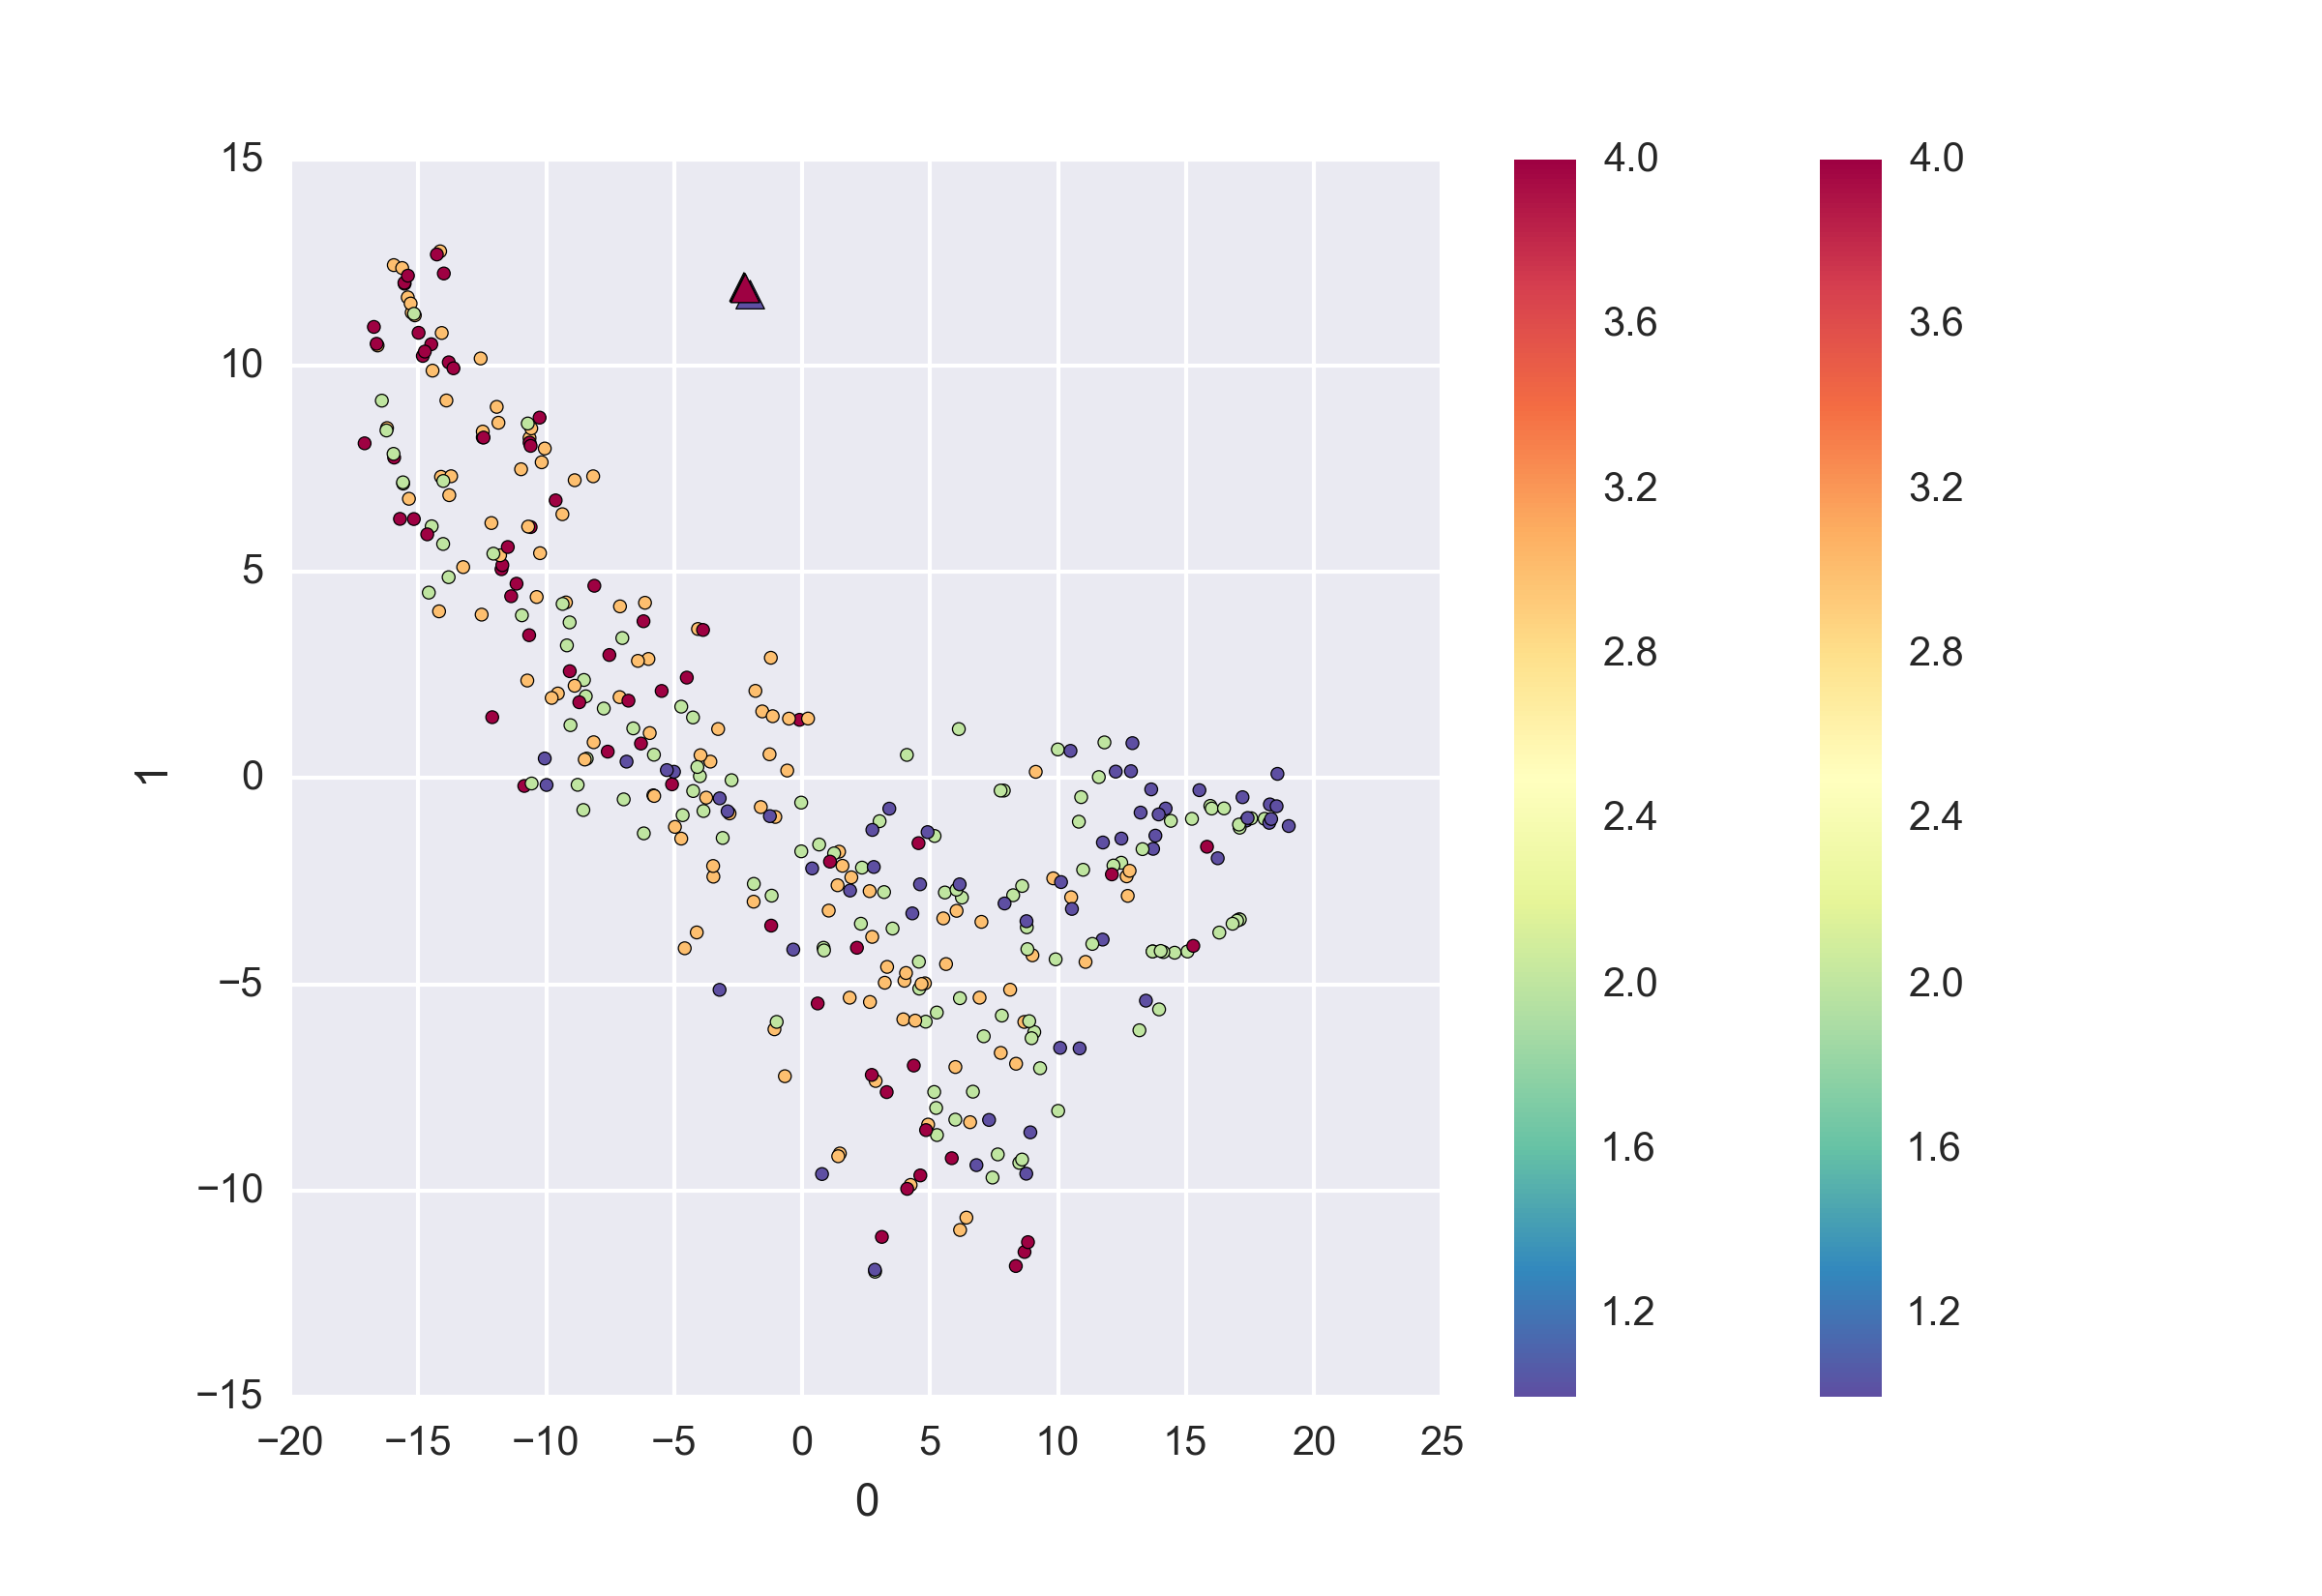
\includegraphics[width=0.49\textwidth]{figures/mappings/texture_SNE_mapping_2d.png}}
	\subfigure{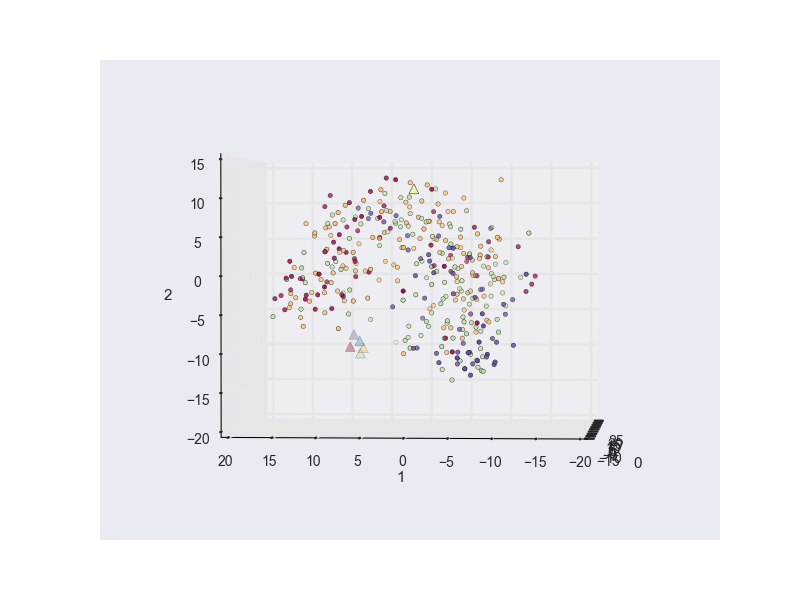
\includegraphics[width=0.49\textwidth]{figures/mappings/texture_SNE_mapping_3d.png}}
	\caption{2D \& 3D projections of the texture feature space generated from blobs generated from blobs produced by the t-SNE algorithm with a learning rate of 300 and perplexity of 30.}\label{fig:texture_SNE_mapping}
\end{figure}

\begin{figure}[H]
	\centering
	\subfigure{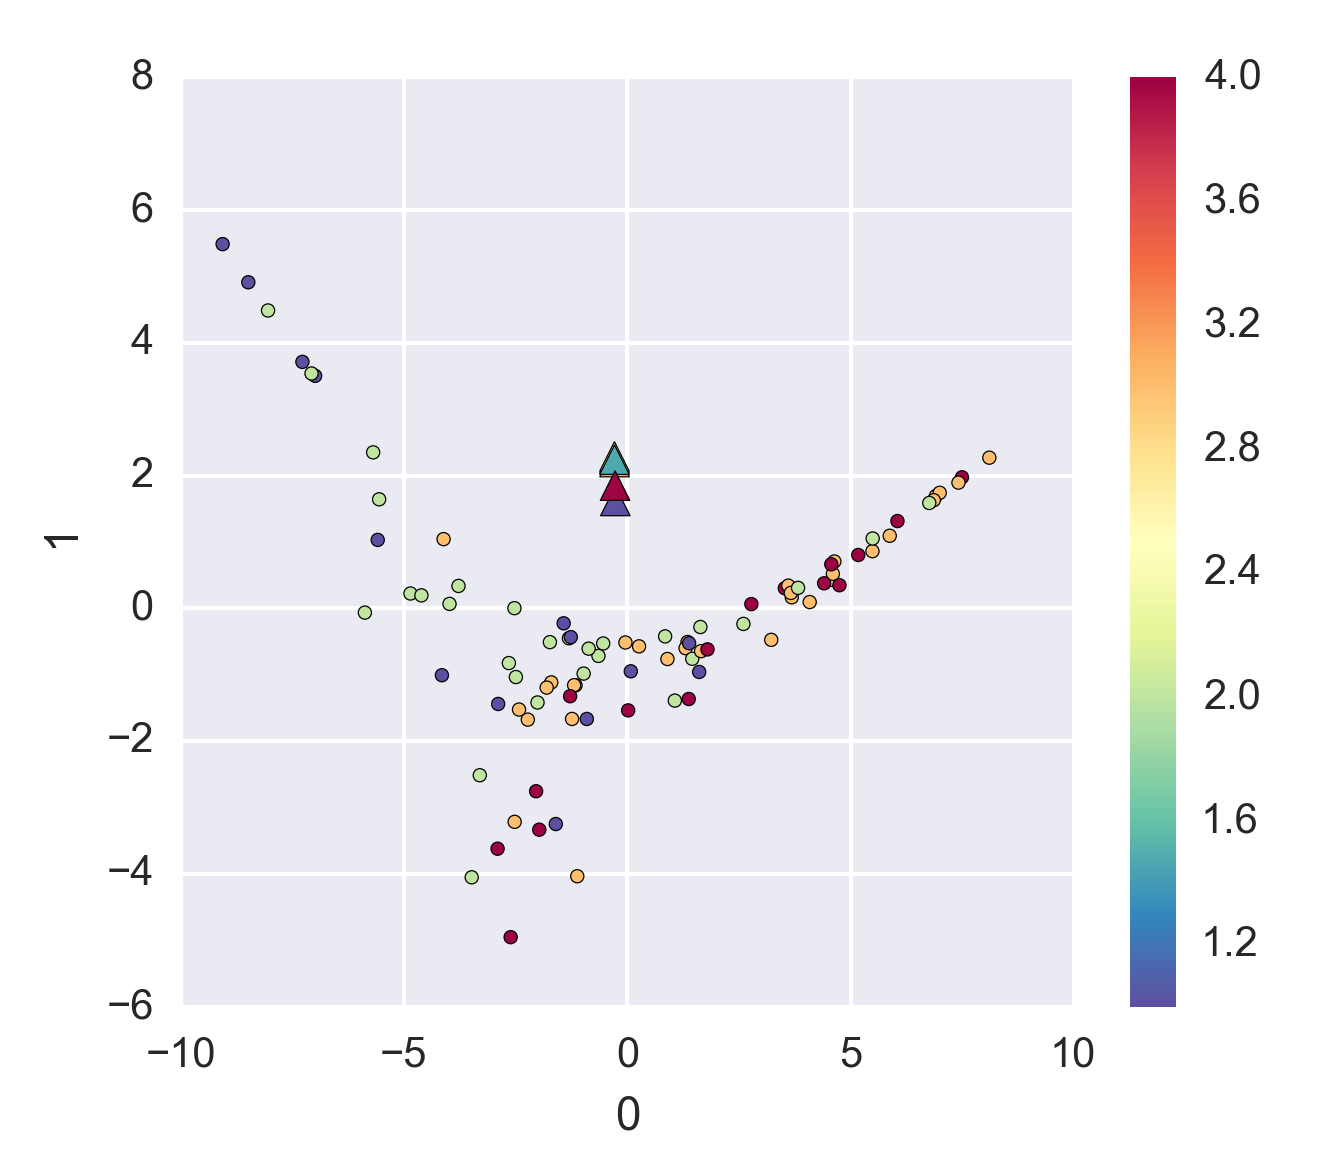
\includegraphics[width=0.49\textwidth]{figures/mappings/texture_iso_mapping_2d.png}}
	\subfigure{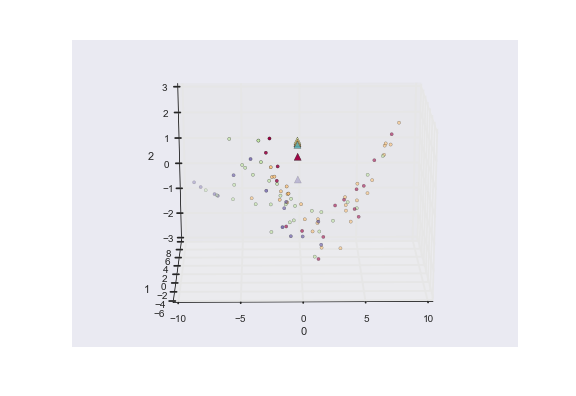
\includegraphics[width=0.49\textwidth]{figures/mappings/texture_iso_mapping_3d.png}}
	\caption{2D \& 3D projections of the texture feature space generated from blobs produced by the Isomap algorithm with 10 neighbours.}\label{fig:texture_iso_mapping}
\end{figure}

\begin{figure}[H]
	\centering
	\subfigure{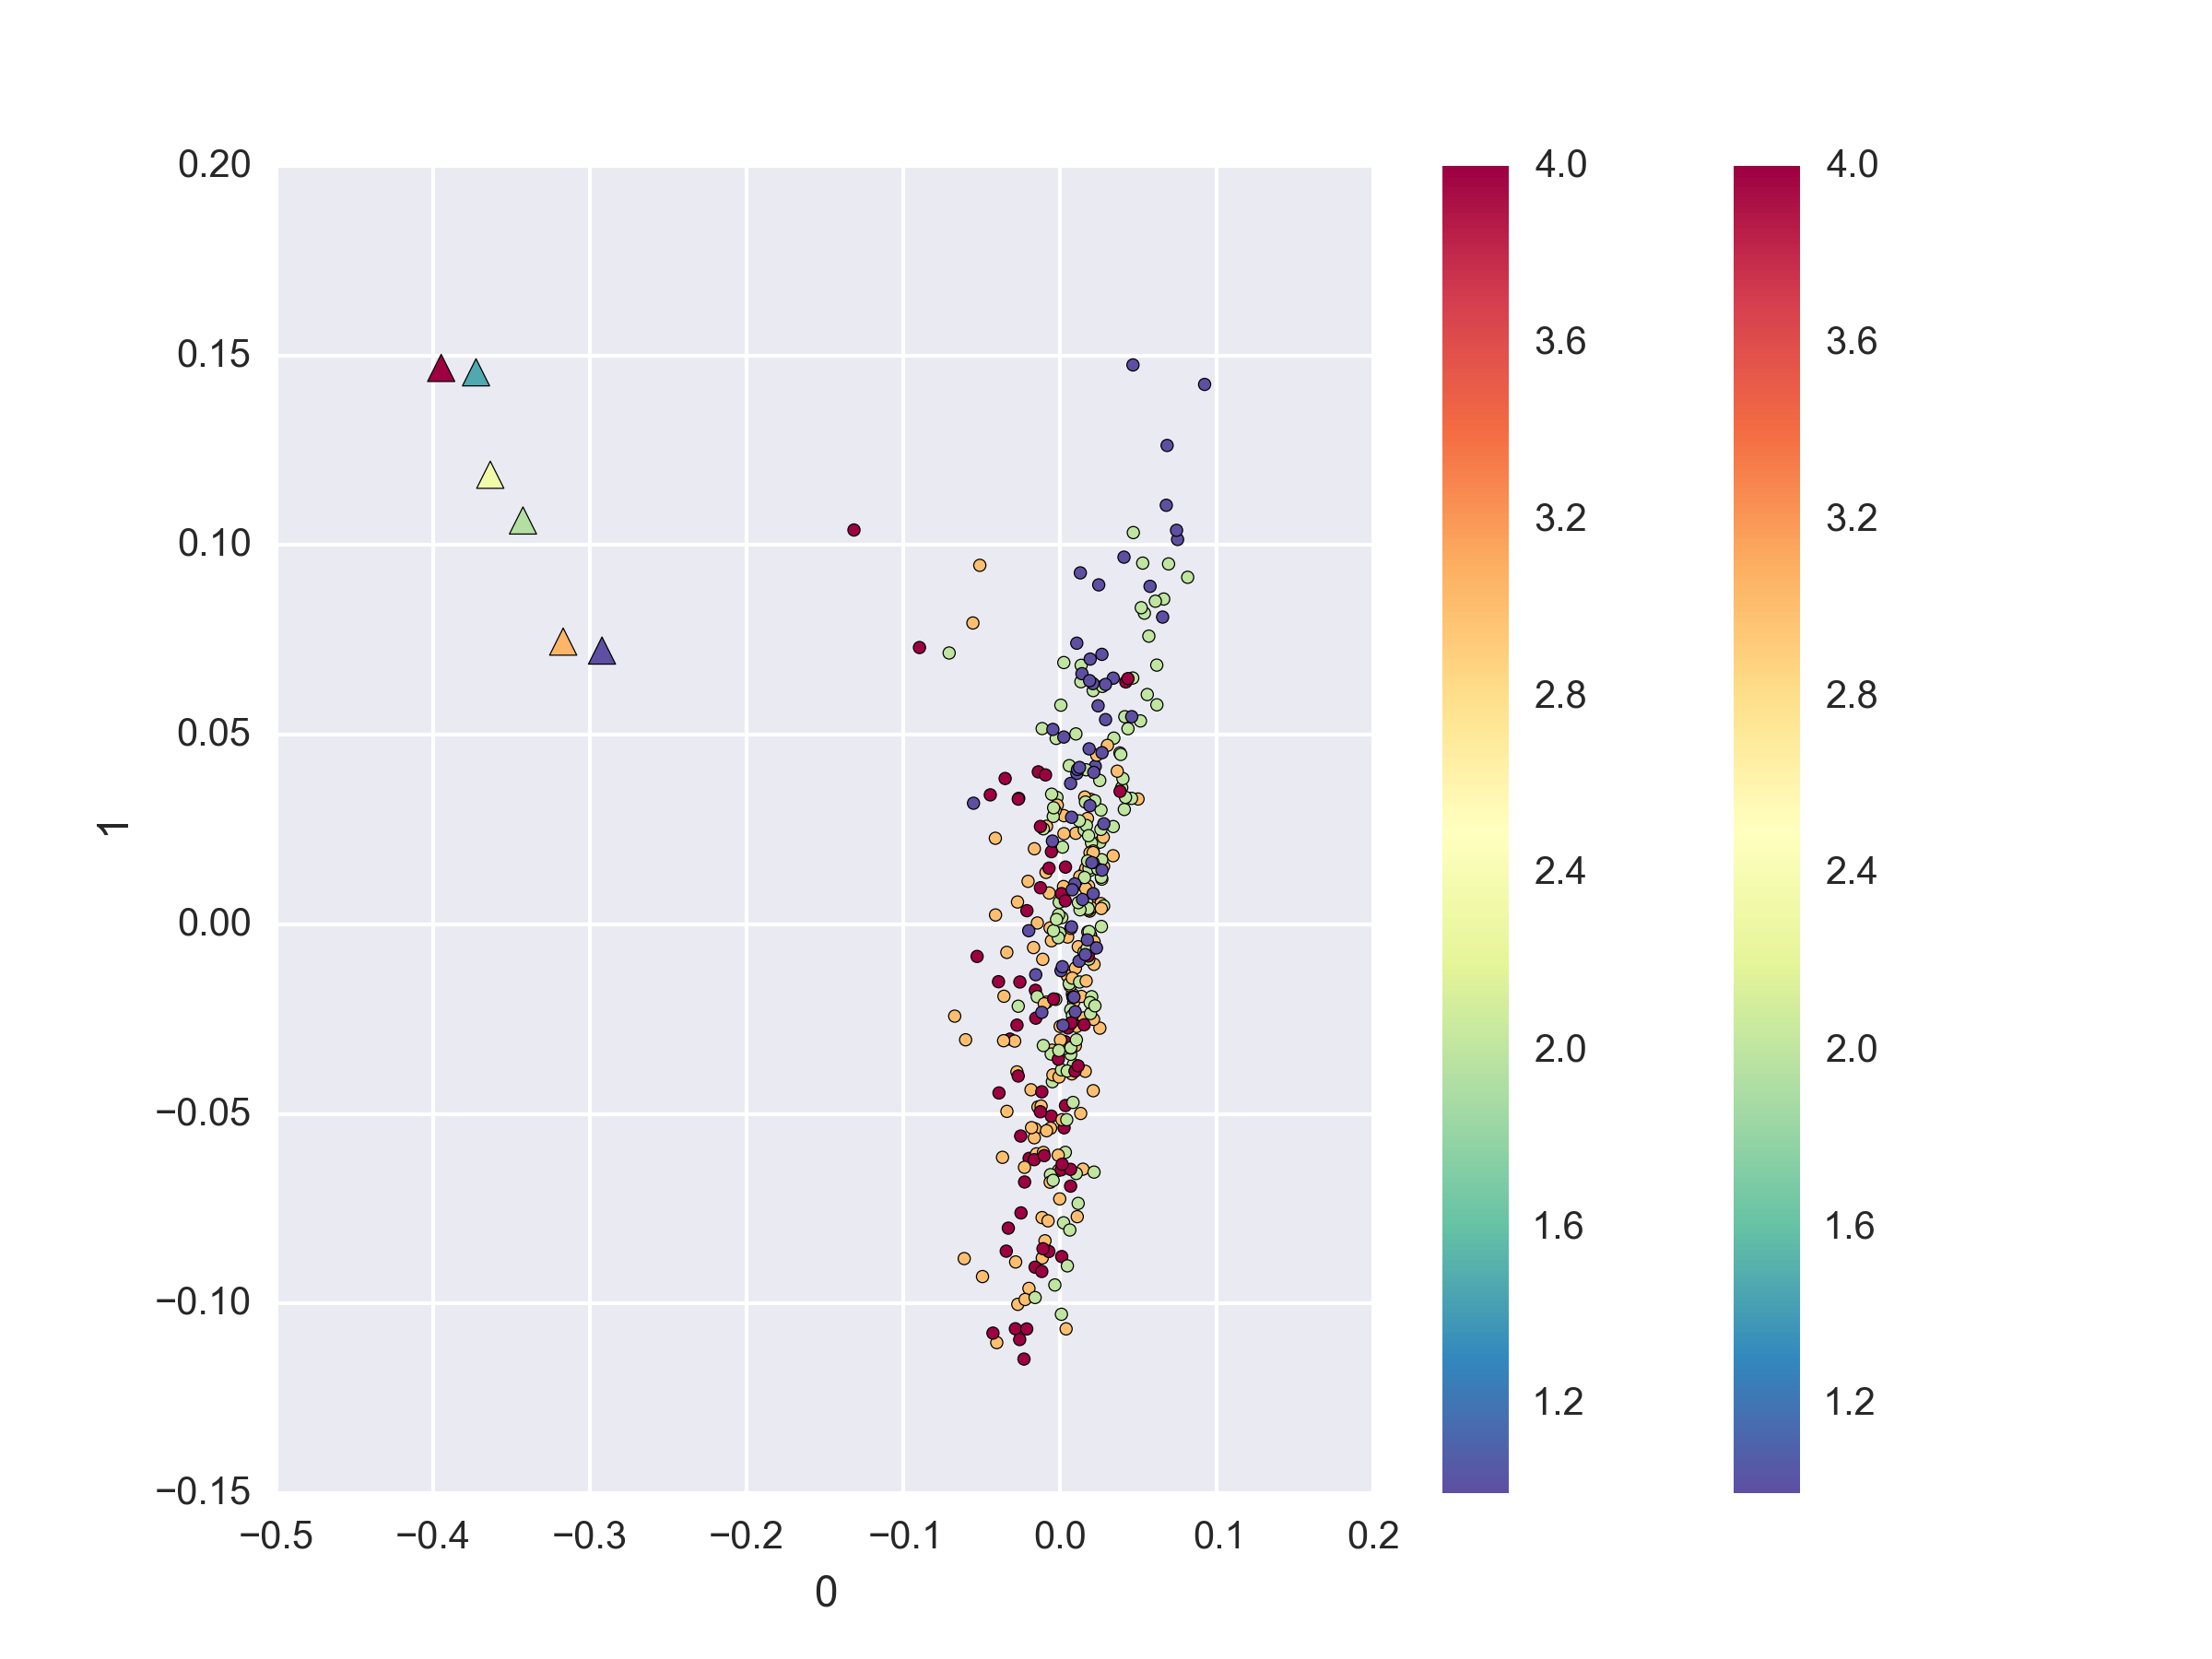
\includegraphics[width=0.49\textwidth]{figures/mappings/texture_lle_mapping_2d.png}}
	\subfigure{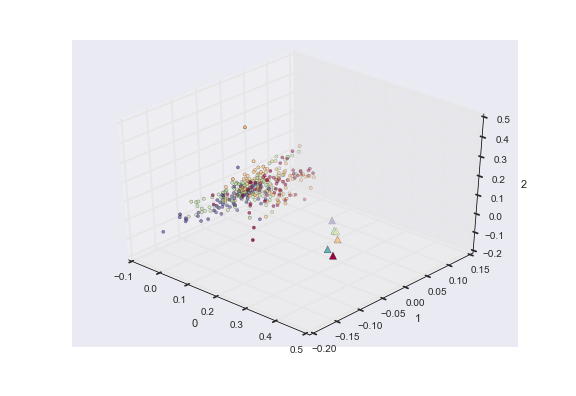
\includegraphics[width=0.49\textwidth]{figures/mappings/texture_lle_mapping_3d.png}}
	\caption{2D \& 3D projections of the texture feature space generated from blobs produced by the LLE algorithm with 10 neighbours.}\label{fig:texture_LLE_mapping}
\end{figure}
\clearpage

% Quality for blob texture features
%------------------------------------------------------------------------------------

\clearpage
\begin{figure}[H]
	\centering
	\subfigure{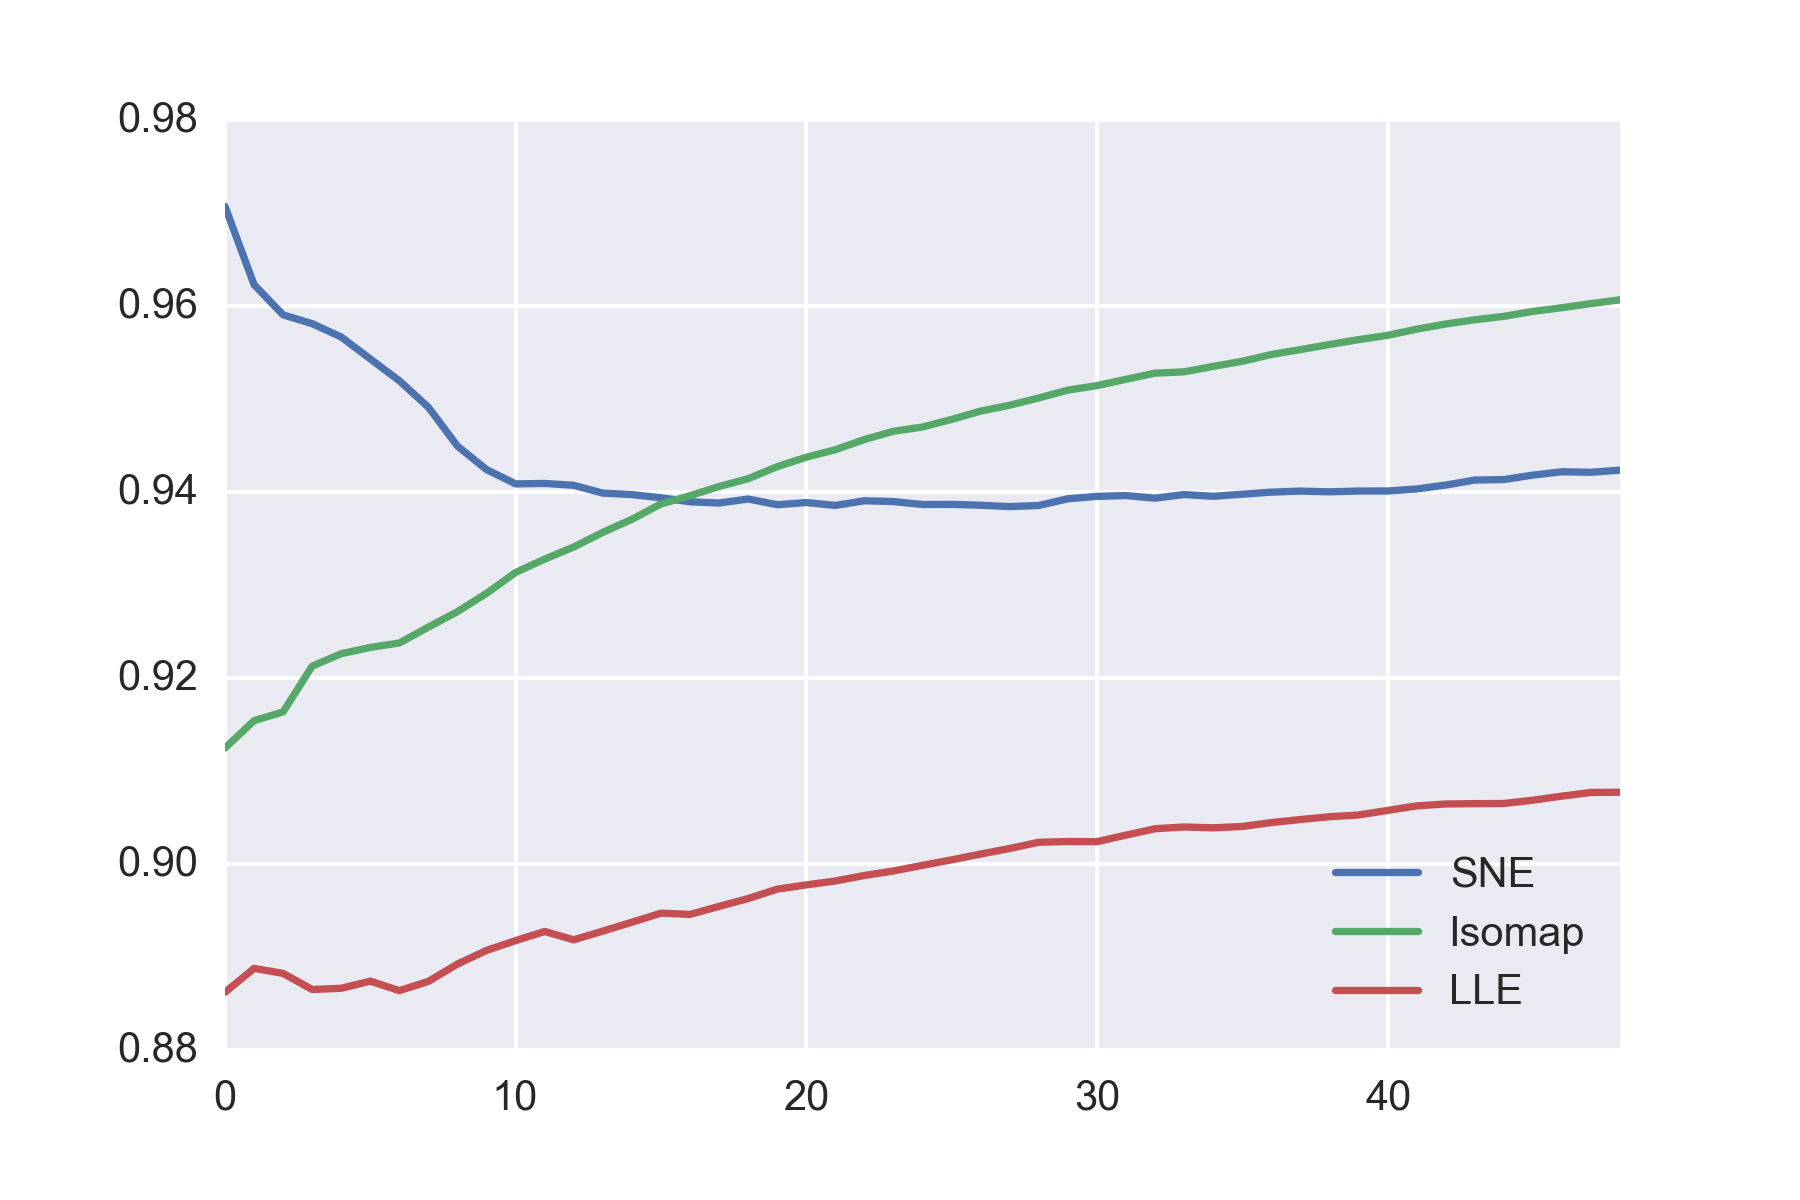
\includegraphics[width=0.49\textwidth]{figures/quality_measures/texture_trustworthiness_2d.png}}
	\subfigure{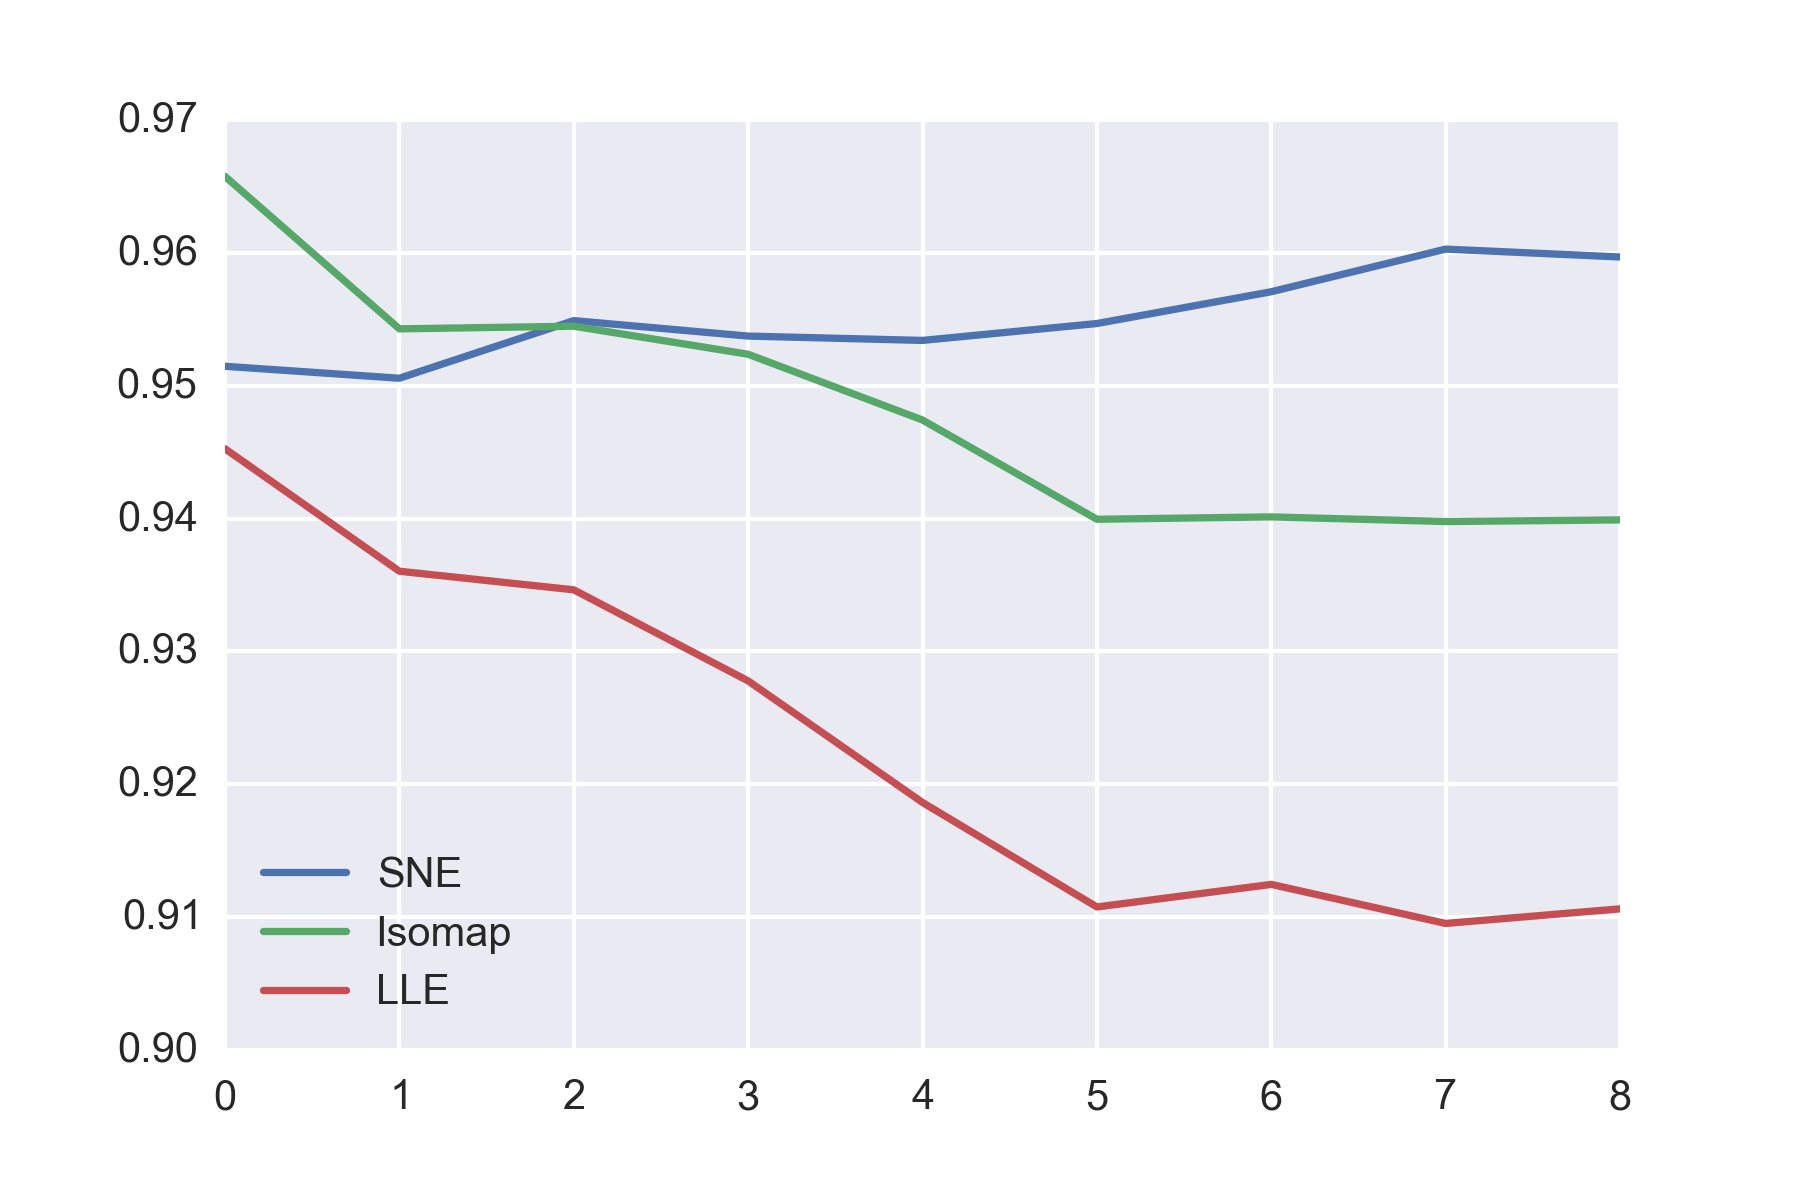
\includegraphics[width=0.49\textwidth]{figures/quality_measures/texture_continuity_2d.png}}
	\caption{Trustworthiness (left) and continuity (right) of the 2D projections produced from texture features from blobs.}\label{fig:TC_2d_texture}
\end{figure}

\begin{figure}[H]
	\centering
	\subfigure{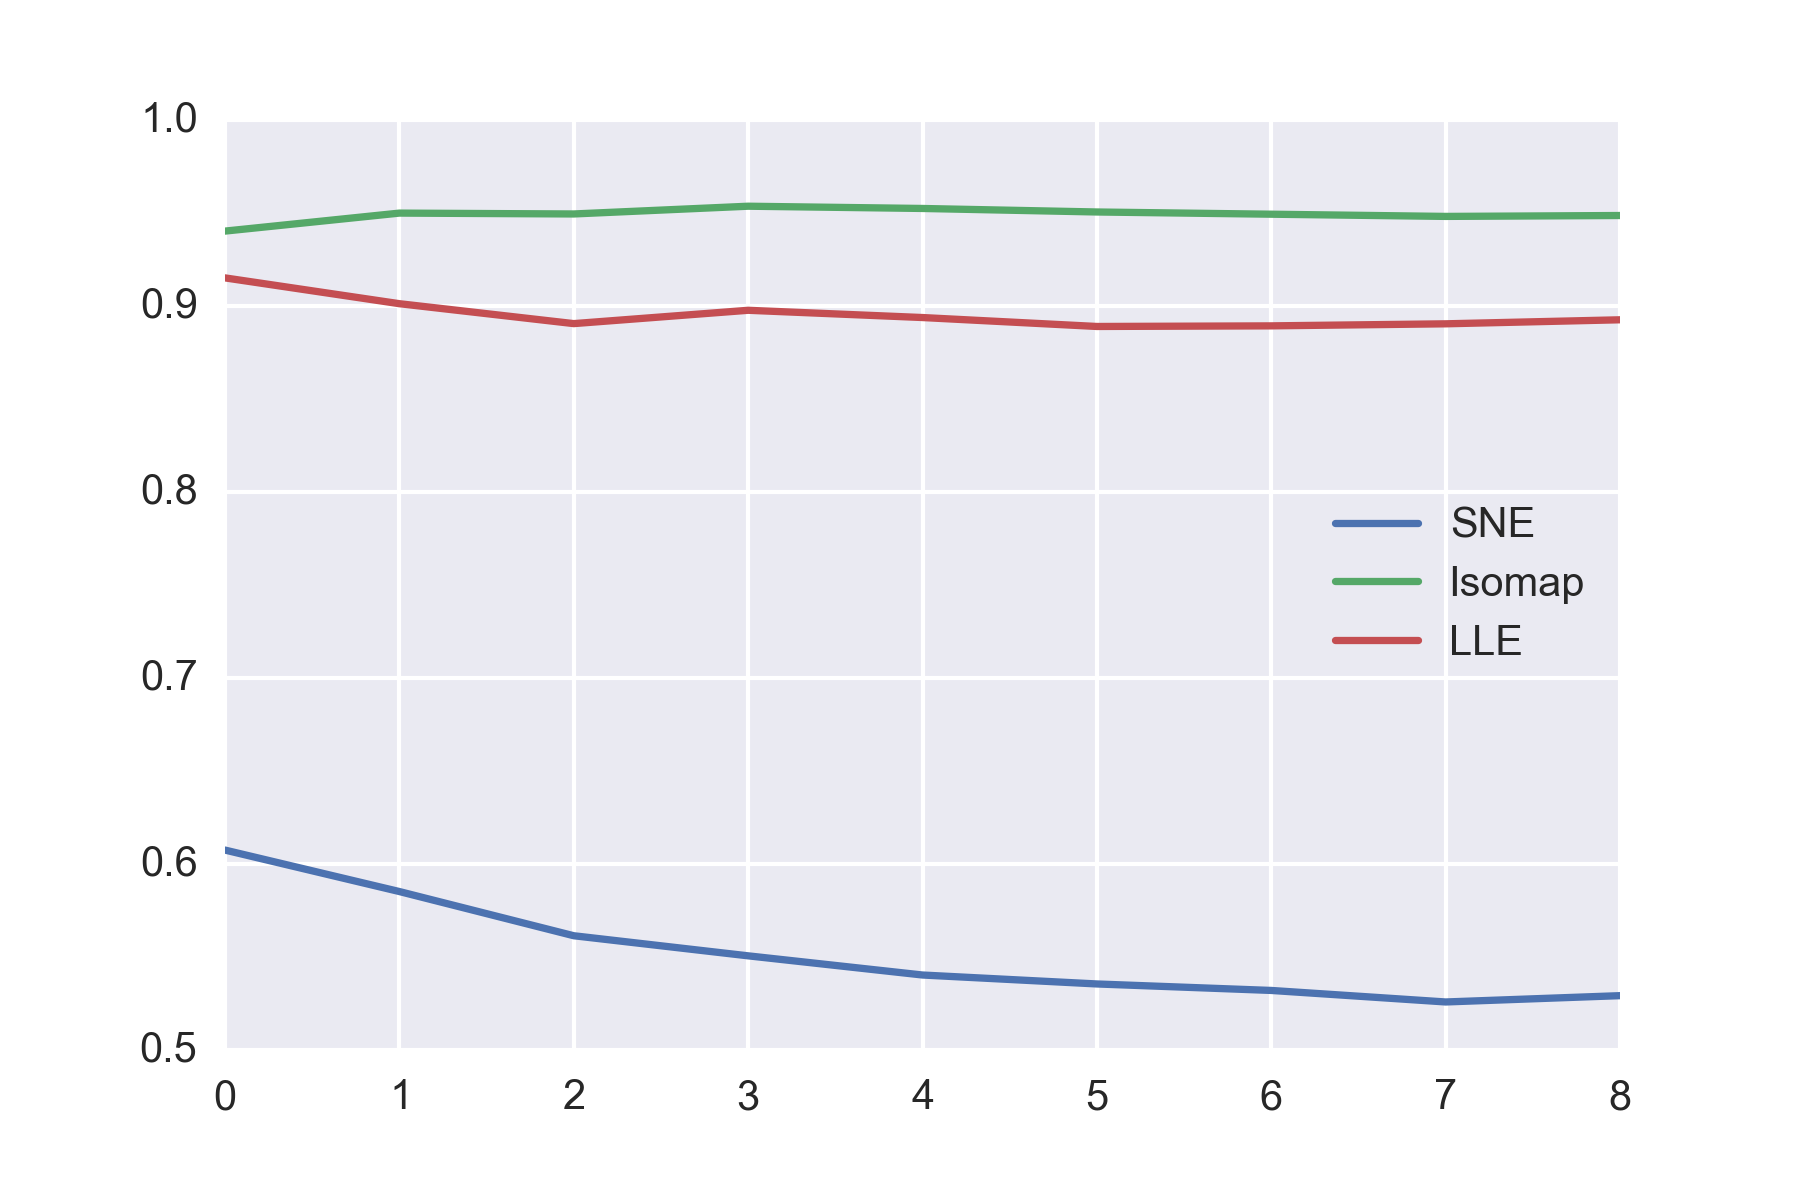
\includegraphics[width=0.49\textwidth]{figures/quality_measures/texture_trustworthiness_3d.png}}
	\subfigure{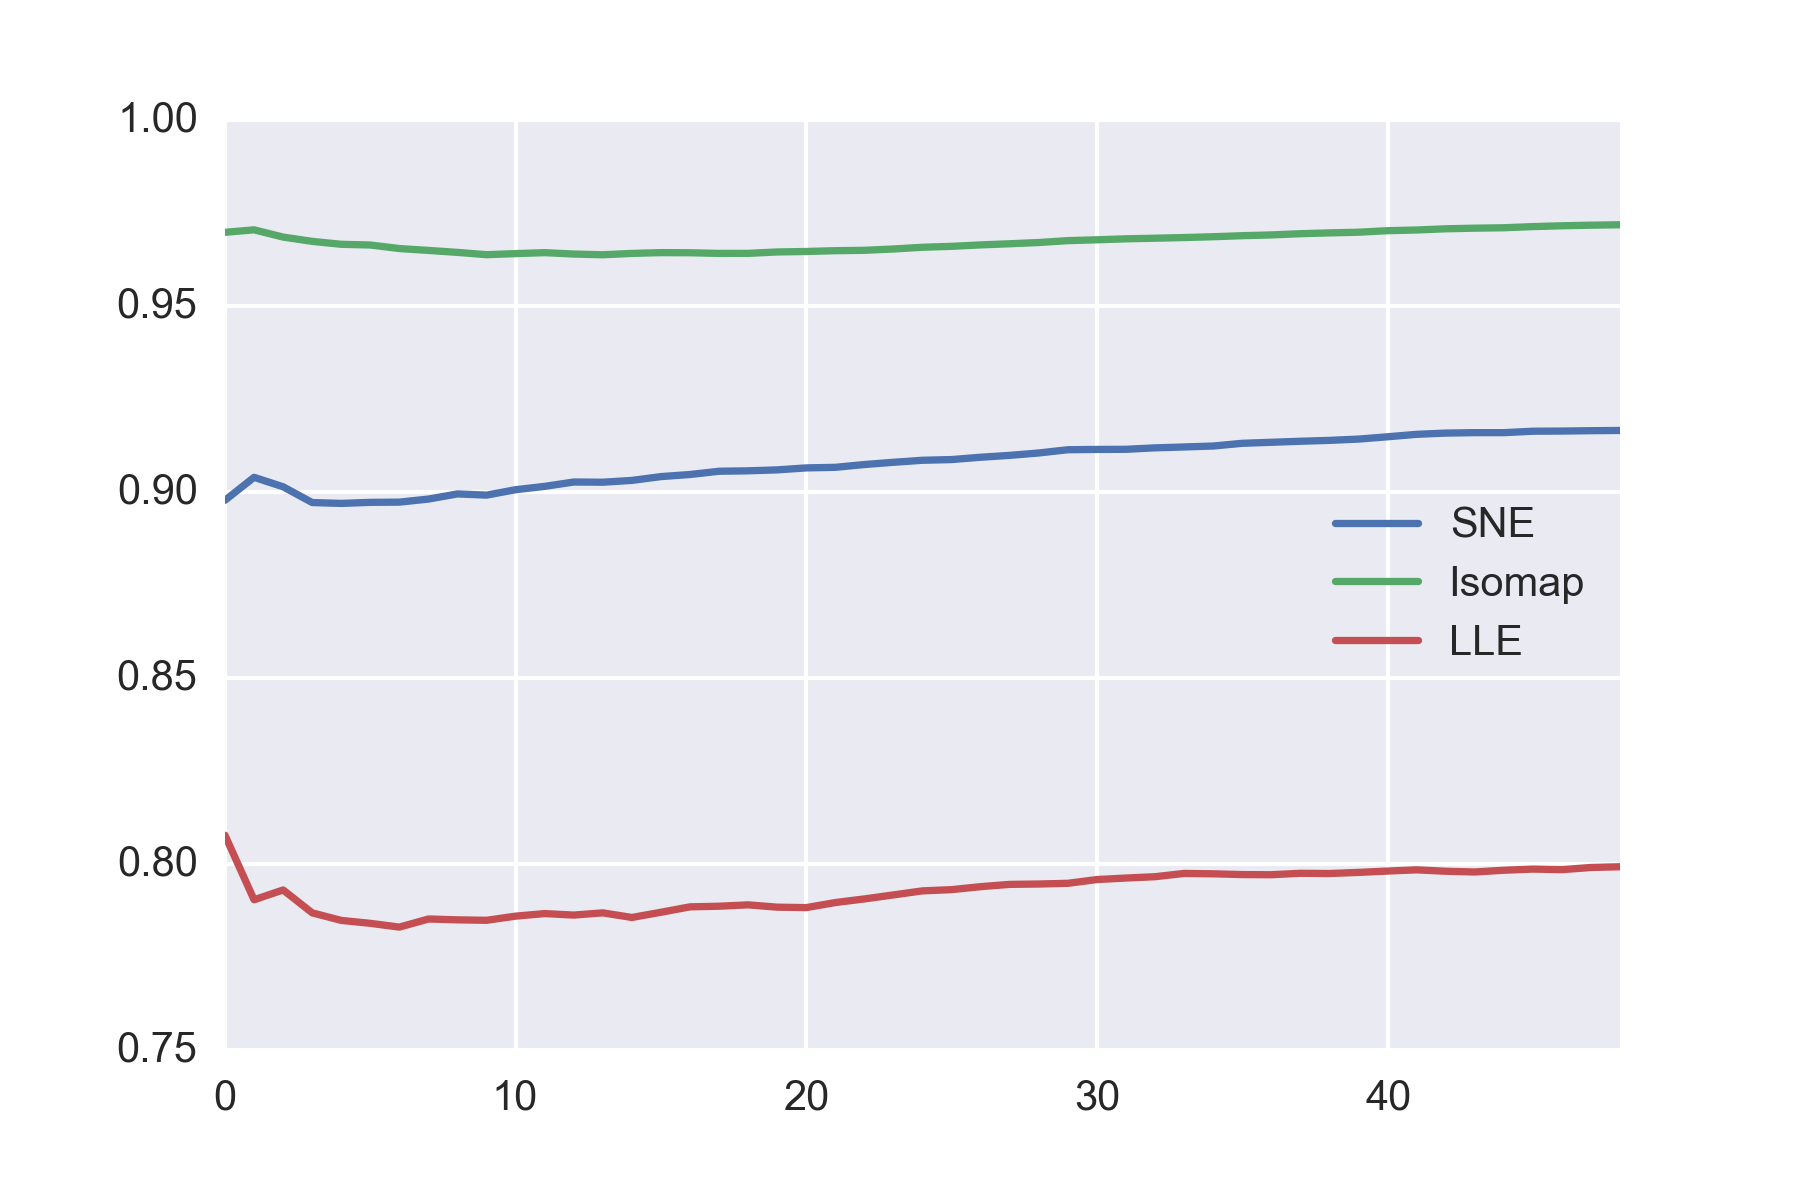
\includegraphics[width=0.49\textwidth]{figures/quality_measures/texture_continuity_3d.png}}
	\caption{Trustworthiness (left) and continuity (right) of the 3D projections produced from texture features from blobs.}\label{fig:TC_3d_texture}
\end{figure}

\begin{figure}[H]
	\centering
	\subfigure{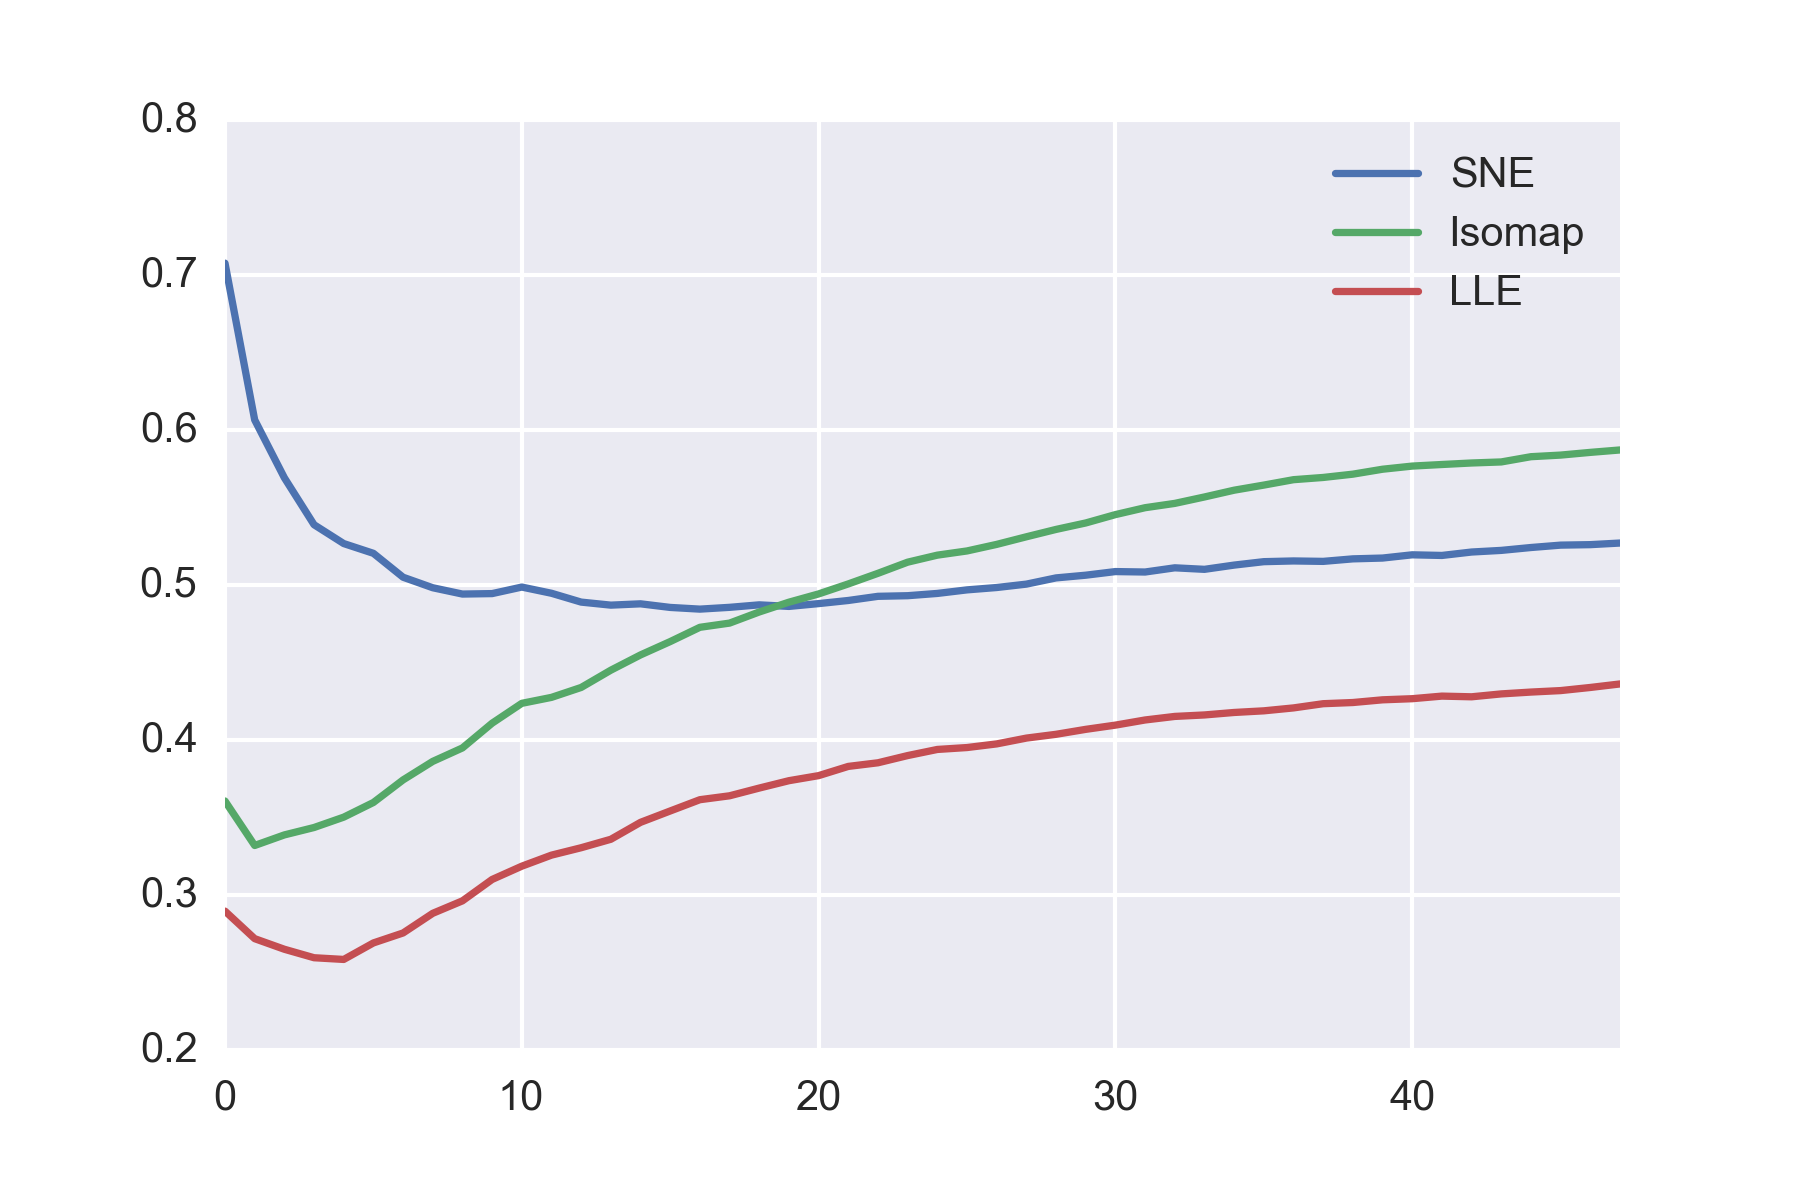
\includegraphics[width=0.49\textwidth]{figures/quality_measures/texture_lcmc_2d.png}}
	\subfigure{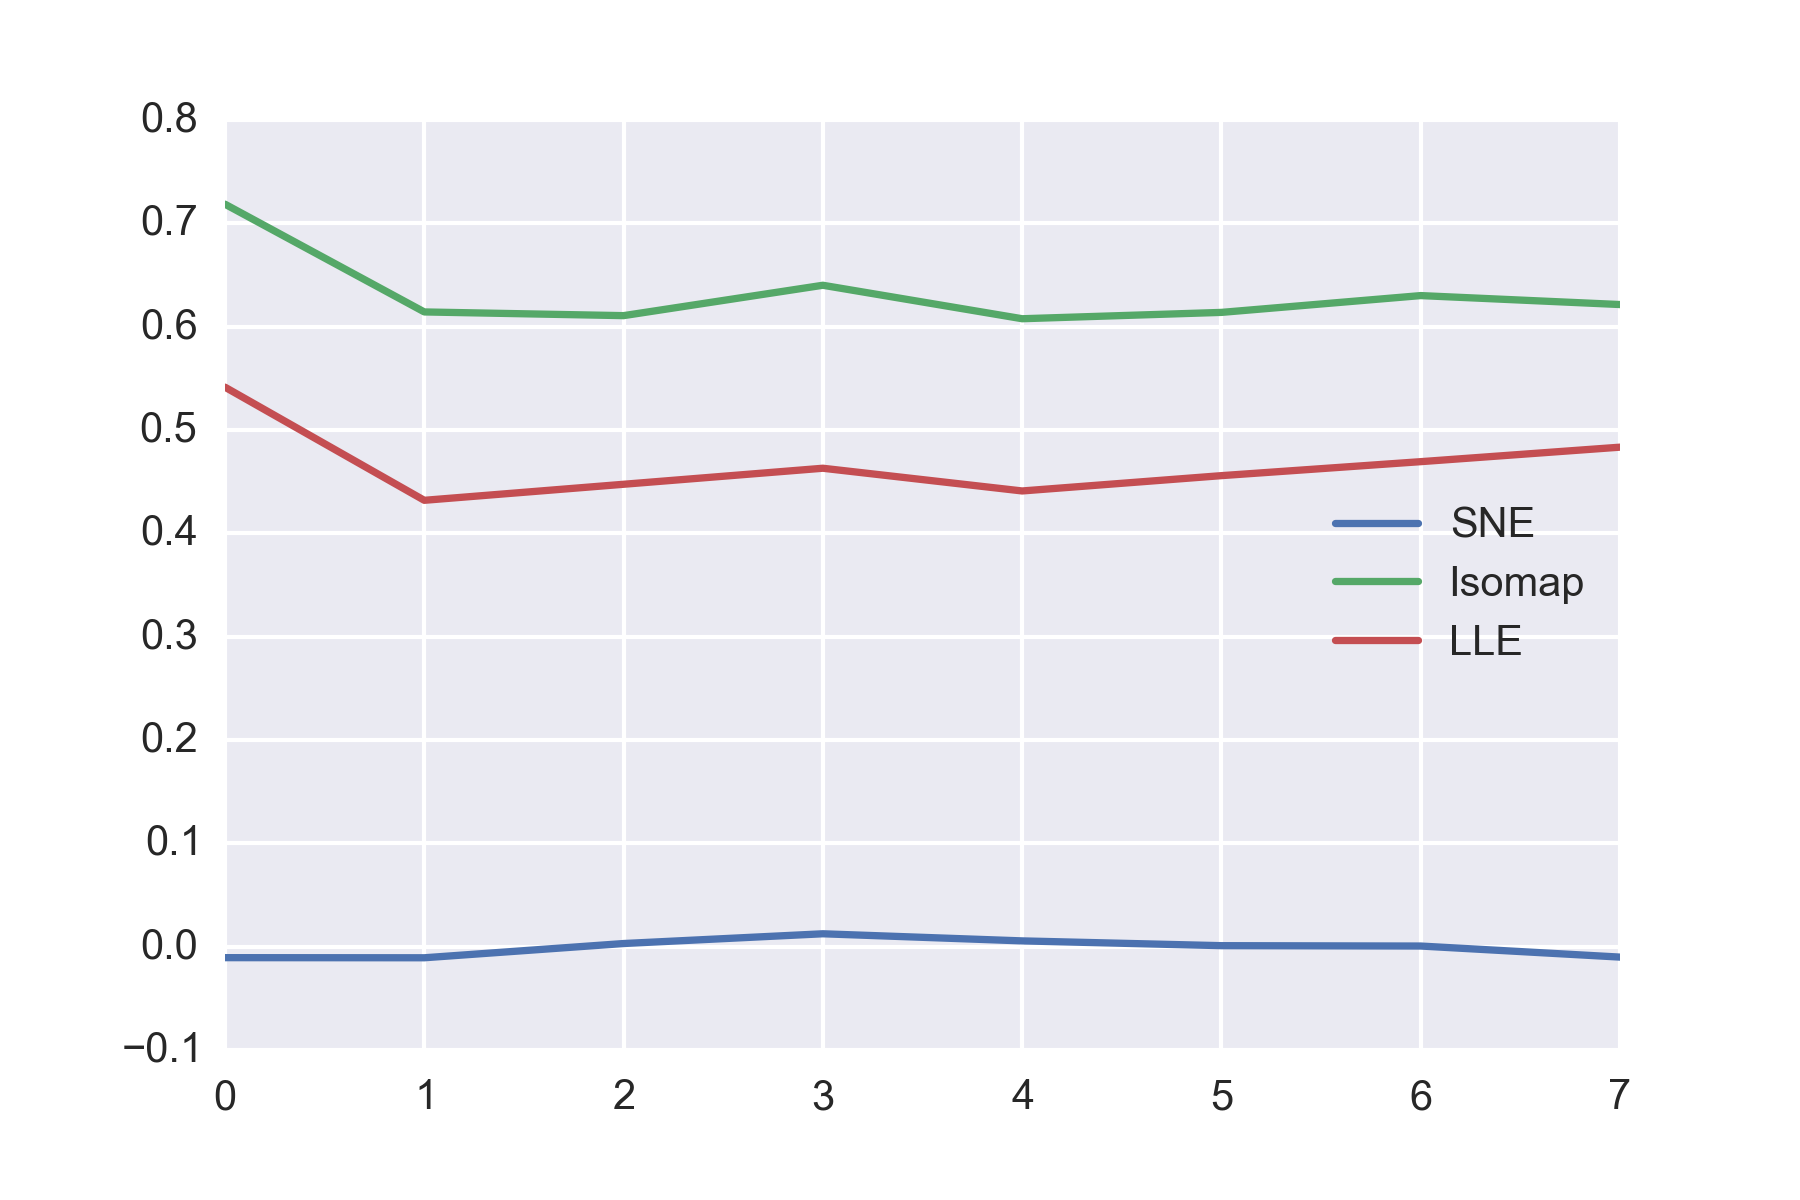
\includegraphics[width=0.49\textwidth]{figures/quality_measures/texture_lcmc_3d.png}}
	\caption{LCMC of both the 2D projection (left) and 3D projection (right) of the feature space for texture.}\label{fig:LCMC_texture}
\end{figure}
\clearpage

%------------------------------------------------------------------------------------
% Line intensity and texture features
%------------------------------------------------------------------------------------

\clearpage
\begin{figure}[H]
	\centering
	\subfigure{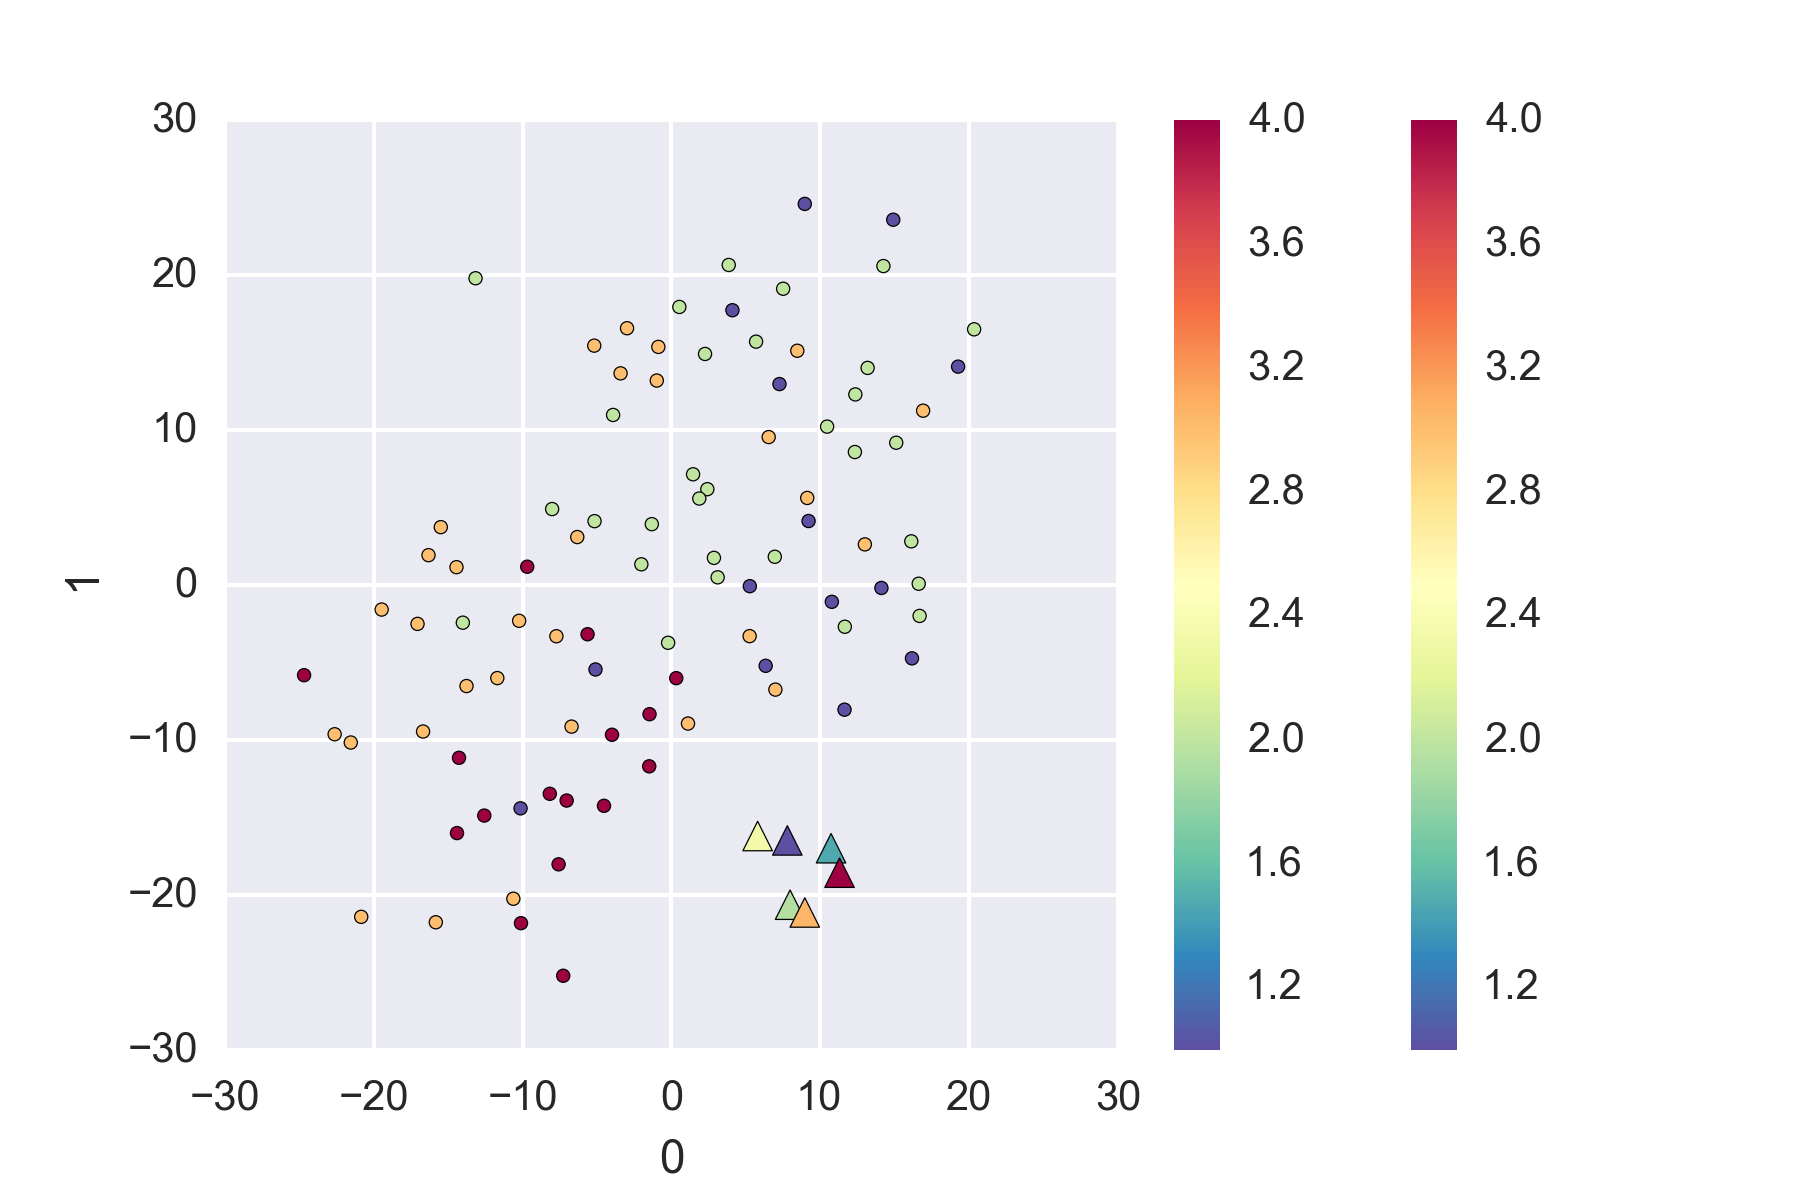
\includegraphics[width=0.49\textwidth]{figures/mappings/line_intensity_SNE_mapping_2d.png}}
	\subfigure{\includegraphics[width=0.49\textwidth]{figures/mappings/line_intensity_SNE_mapping_3d.png}}
	\caption{2D \& 3D projections of the intensity feature space for lines produced by the t-SNE algorithm with a learning rate of 300 and perplexity of 30.}\label{fig:intensity_SNE_mapping_lines}
\end{figure}

\begin{figure}[H]
	\centering
	\subfigure{\includegraphics[width=0.49\textwidth]{figures/mappings/line_intensity_iso_mapping_2d.png}}
	\subfigure{\includegraphics[width=0.49\textwidth]{figures/mappings/line_intensity_iso_mapping_3d.png}}
	\caption{2D \& 3D projections of the intensity feature space generated from lines produced by the Isomap algorithm with 10 neighbours.}\label{fig:intensity_iso_mapping_lines}
\end{figure}

\begin{figure}[H]
	\centering
	\subfigure{\includegraphics[width=0.49\textwidth]{figures/mappings/line_intensity_lle_mapping_2d.png}}
	\subfigure{\includegraphics[width=0.49\textwidth]{figures/mappings/line_intensity_lle_mapping_3d.png}}
	\caption{2D \& 3D projections of the intensity feature space for lines generated from blobs produced by the LLE algorithm with 50 neighbours.}\label{fig:intensity_LLE_mapping_lines}
\end{figure}
\clearpage


% Quality for line intensity features
%------------------------------------------------------------------------------------
\clearpage
\begin{figure}[H]
	\centering
	\subfigure{\includegraphics[width=0.49\textwidth]{figures/quality_measures/line_intensity_trustworthiness_2d.png}}
	\subfigure{\includegraphics[width=0.49\textwidth]{figures/quality_measures/line_intensity_continuity_2d.png}}
	\caption{Trustworthiness (left) and continuity (right) of the 2D projections produced from intensity features from lines.}\label{fig:TC_2d_intensity}
\end{figure}

\begin{figure}[H]
	\centering
	\subfigure{\includegraphics[width=0.49\textwidth]{figures/quality_measures/line_intensity_trustworthiness_3d.png}}
	\subfigure{\includegraphics[width=0.49\textwidth]{figures/quality_measures/line_intensity_continuity_3d.png}}
	\caption{Trustworthiness (left) and continuity (right) of the 3D projections produced from intensity features from lines.}\label{fig:TC_3d_intensity}
\end{figure}

\begin{figure}[H]
	\centering
	\subfigure{\includegraphics[width=0.49\textwidth]{figures/quality_measures/line_intensity_lcmc_2d.png}}
	\subfigure{\includegraphics[width=0.49\textwidth]{figures/quality_measures/line_intensity_lcmc_3d.png}}
	\caption{LCMC of both the 2D projection (left) and 3D projection (right) of the feature space for intensity from lines.}\label{fig:LCMC_intensity}
\end{figure}
\clearpage


\clearpage
\begin{figure}[H]
	\centering
	\subfigure{\includegraphics[width=0.49\textwidth]{figures/mappings/lines_texture_SNE_mapping_2d.png}}
	\subfigure{\includegraphics[width=0.49\textwidth]{figures/mappings/lines_texture_SNE_mapping_3d.png}}
	\caption{2D \& 3D projections of the texture feature space generated generated from lines produced by the t-SNE algorithm with a learning rate of 300 and perplexity of 30.}\label{fig:texture_SNE_mapping_lines}
\end{figure}

\begin{figure}[H]
	\centering
	\subfigure{\includegraphics[width=0.49\textwidth]{figures/mappings/lines_texture_iso_mapping_2d.png}}
	\subfigure{\includegraphics[width=0.49\textwidth]{figures/mappings/lines_texture_iso_mapping_3d.png}}
	\caption{2D \& 3D projections of the texture feature space generated from lines produced by the Isomap algorithm with 10 neighbours.}\label{fig:texture_iso_mapping_lines}
\end{figure}

\begin{figure}[H]
	\centering
	\subfigure{\includegraphics[width=0.49\textwidth]{figures/mappings/lines_texture_lle_mapping_2d.png}}
	\subfigure{\includegraphics[width=0.49\textwidth]{figures/mappings/lines_texture_lle_mapping_3d.png}}
	\caption{2D \& 3D projections of the texture feature space generated from lines produced by the LLE algorithm with 10 neighbours.}\label{fig:texture_LLE_mapping_lines}
\end{figure}
\clearpage

% Quality for line texture features
%------------------------------------------------------------------------------------

\clearpage
\begin{figure}[H]
	\centering
	\subfigure{\includegraphics[width=0.49\textwidth]{figures/quality_measures/lines_texture_trustworthiness_2d.png}}
	\subfigure{\includegraphics[width=0.49\textwidth]{figures/quality_measures/lines_texture_continuity_2d.png}}
	\caption{Trustworthiness (left) and continuity (right) of the 2D projections produced from texture features from lines.}\label{fig:TC_2d_texture}
\end{figure}

\begin{figure}[H]
	\centering
	\subfigure{\includegraphics[width=0.49\textwidth]{figures/quality_measures/lines_texture_trustworthiness_3d.png}}
	\subfigure{\includegraphics[width=0.49\textwidth]{figures/quality_measures/lines_texture_continuity_3d.png}}
	\caption{Trustworthiness (left) and continuity (right) of the 3D projections produced from texture features from lines.}\label{fig:TC_3d_texture}
\end{figure}

\begin{figure}[H]
	\centering
	\subfigure{\includegraphics[width=0.49\textwidth]{figures/quality_measures/lines_texture_lcmc_2d.png}}
	\subfigure{\includegraphics[width=0.49\textwidth]{figures/quality_measures/lines_texture_lcmc_3d.png}}
	\caption{LCMC of both the 2D projection (left) and 3D projection (right) of the feature space from lines for texture.}\label{fig:LCMC_texture}
\end{figure}
\clearpage


\section{Conclusions}
In summary, it can be concluded that the synthetic mammograms used as part of this experiment are not significantly related to real mammograms in terms of the features derived during this study. The synthetic mammograms appear to be closest to real mammograms in terms of the shape of the structures present in the image. The best results from this experiment were derived from the feature space of multi-scale blobs. Line features also seemed to positively show the the real and synthetic mammograms are at least in the same space in terms of shape. However, texture and intensity features derived from either of the features clearly show that the two datasets are not in the same intensity space. The two sample KS test confirms that the features created from both datasets are statistically not drawn from the same distribution and therefore we must conclude that they are, for all features presented here, effectively different.

This conclusion roughly correlates with the limitations discussed by the authors of the synthetic data \cite{bakic2002mammogram1, bakic2002mammogram2, bakic2003mammogram3}. They state that the synthetic mammograms are closest to real mammograms in terms of shape but are not so close in terms of intensity and texture. In the experiments with shape features presented here the major difference between the real and synthetic mammograms was caused by a lack of small scale structure being detected in the synthetic mammograms. This causes them to be grouped in with mammograms which are deemed to be of higher risk, regardless of their effective risk, because of the lack of small blob counts detected. The same can be said for line features where the number and size of lines is generally smaller, regardless of the risk.

The quality evaluation of the visualisations produced suggests that t-SNE produces visualisations which best capture the local neighbourhood structure in for a small local neighbourhood, but that Isomap generally performs better across most feature spaces as $k$ increases. This does appear to coincide with expectations about what the two algorithms aim to preserve. t-SNE is typically better at preserving the local relationship of a neighbourhood and Isomap better for the global structure. LLE is shown to generally produce better visualisations when $k$ is small and degrades as the neighbourhood becomes larger. However it was typically shown to produce a lower quality of embedding in comparison to t-SNE.


